\documentclass{puthesis}
\usepackage{times}
\usepackage{listings}
\usepackage[chapter]{algorithm}
\usepackage{algorithmic}
\usepackage{amsfonts}
\usepackage{amsmath}
\usepackage{graphicx}
\usepackage{subfigure}
\usepackage{tabularx}
\usepackage{booktabs}
\usepackage[symbol]{footmisc}
\doublespacing
\usepackage{fancyhdr}
\usepackage{lscape}
\usepackage{cases}
\usepackage{url}
\usepackage{enumerate}

\renewcommand{\algorithmicrequire}{\textbf{Given:}}
\renewcommand{\algorithmicensure}{\textbf{Goal:}}
%\renewcommand{\labelitemi}{$\diamond$}

\def\bez{B\'ezier\ }
\def\be{\begin{equation}}
\def\ee{\end{equation}}
\newcommand{\bt}{{\bf t}}
\newcommand{\bu}{{\bf u}}
\newcommand{\bv}{{\bf v}}
\newcommand{\bs}{{\bf S}}
\newcommand{\jfair}{J_{fair}(\bs)}
\newcommand{\myvec}[4]{#1_#2,#1_#3,\cdots,#1_#4}
%\newcommand{\mybracket}{]}




%%%%%%%%%%%%%%%%%%%%%%%%%%%%%%%%%%%%%%%%%
%%%%%%%%%%%%%%%%%%%%%%%%%%%%%%%%%%%%%%%%%
\author{WANG KAI}

%%%%%%%%%%%%%%%%%%%%%%%%%%%%%%%%%%%%%%%%%
%%%%%%%%%%%%%%%%%%%%%%%%%%%%%%%%%%%%%%%%%
\abstract{ This research investigates the use of sketching
techniques  in 3D modeling and reconstruction to enhance various
processes such as 3D model creation, editing, analyzing and
computing. 3D geometric models have been widely used in various
applications from industrial design to digital entertainment.
However, creating and processing 3D models with traditional 2D
WIMP-style (Windows, Icon, Menu, Pointer) interfaces are generally
tedious and time-consuming. On the other hand, sketching interfaces
are emerging as a new approach to enhance user interactions for
various design activities. The sketching interfaces are expected to
provide flexible and intuitive interactions between computers and
users. To effectively incorporated the sketching techniques into 3D
modeling and reconstruction, some fundamental theories and
supporting algorithms should be developed. The goal of this research
is thus to investigate how to create intuitive and effective
sketching interfaces and meanwhile to develop sketch-based
techniques for creating and editing 3D geometric models.

Firstly, we develop a reference  plane assisted sketching interface
for freeform shape design, in which users can create and edit 3D
models through simple sketches. To regularize and interpret the user
input properly when sketching the shape of the 3D object, we
introduce some rules for the strokes into the system, which consider
both the semantic meaning of the sketched strokes and human
psychology. To make 3D location and orientation of strokes
meaningful and intuitive within 2D interface, we propose to perform
the modeling operations with reference to some auxiliary planes,
which are automatically constructed based on the user sketches or
default setting. The use of reference planes helps to make the
sketch-based modeling system more intuitive and easy to use.
%Third, we also propose a local refinement scheme for triangular meshes to improve the quality of the constructed mesh, especially after large deformation. This sketching system also serves as a platform to test various digital geometry processing algorithms for our research.

Secondly, we propose a  progressive modeling approach to allow users
to create a 3D model with arbitrary topology through iterative
sketches, by taking both the existing sketched curves and the
up-to-date reconstructed model as references. In this way, users
get aware of the shape of the sketched model, which helps to avoid
unexpected modeling result. To effectively support this modeling
approach, we present a CSG-based surface reconstruction algorithm
that enables gradual shape updates and produces models with a single
connected component when the user iteratively adds new sketches. By
using this progressive modeling approach in the sketching interface,
the creation function  will become more powerful in producing a
desired 3D shape by sketching iteratively from scratch, and ambiguities
on perception of the sketched shape can be avoided to a large
extent.

Thirdly, we propose an  edge-based flexible mesh deformation algorithm
to effectively support the editing function in our sketch-based
modeling system. An edge-based graph is proposed for a triangular
mesh, which makes more points get involved in the evaluation of
shape of the mesh surface and thus renders more accurate computation
results. Based on the edge-based graph, we develop a flexible mesh
deformation algorithm which gives users flexibility to adjust the
deformation effects between local shape preservation and global
smoothness through manipulating a simple balance parameter. This
scheme is also applied to local parts of a mesh, to approximate the
deformation effect of real-world objects with non-uniformly
distributed materials. In this way, the deformation process in the
sketch-based modeling  will become more flexible and effective for
users to produce a satisfactory modeling result.

Finally, we apply  the sketching technique to tackle the problem of
surface reconstruction from general cross section curves. A new
framework  is proposed to build a smooth mesh surface from cross
sections with arbitrary orientations. The framework consists of two
parts. The first part generalizes the algorithm in our progressive
modeling to reconstruct surfaces  interpolating the input cross
sections with arbitrary orientations and having regular local
shapes. The second part allows users to edit the local topology
of the reconstructed model through simple sketches, if the initial
one is not satisfactory. It makes use of the intermediate
information obtained in the first part and thus avoids complicated
analysis and computations. Our framework has the unique property of
producing a manifold surface with only one connected component,
which is usually desired in practice. It can be used in many
geometric modeling tasks, including sketch-based modeling.

}

%%%%%%%%%%%%%%%%%%%%%%%%%%%%%%%%%%%%%%%%%
%%%%%%%%%%%%%%%%%%%%%%%%%%%%%%%%%%%%%%%%%
\acknowledgements{
First and foremost, I would like to thank my supervisor Prof. Zheng Jianmin, for his patient instructions and constant support on this research. His great insight and knowledge always guide me stepping forward and getting out of confusions and frustrations, and his serious attitude helps me to keep on improving the quality of the research work. I believe the things I learned from him will benefit me a lot in my future development. I also thank Prof. Seah Hock-Soon for his instructions and support on my research. I deeply appreciate their encouragement and sincerely hope that our cooperation will continue in the future.

I should appreciate the financial support for this research provided by the National Research Foundation grant, which is administrated by the Media Development Authority Interactive Digital Media Programme Office, and the space and equipment provided by GameLab, Nanyang Technological University.

It is a great pleasure to have the useful cooperations, discussions and funs with my following colleagues and friends in the past four years: Dr. Wang Yimin, Dr. Pan Jianjiang, Dr. Chen Xiaodiao, Dr. Chen Wenyu, Dr. Xin Shiqing, Dr. Li Xin, Dr. Cao Juan, Ma Yuewen, Zhou Hailing, Wu Xiaoqun, Li Yusha, Zhao Ming, Chen Shuangmin, Zhang Wenjing, and Zhang Yuzhe.

Deep thanks to Prof. Wu Zhongke and Prof. Tian Feng for providing me the chance to come to Singapore and see the world. I also appreciate the encouragement and valuable opinions on my career development from Prof. Zhao Zhiwen and Prof. Yao Li.

I would like to extend the deepest appreciations to my parents and my wife, for their constant and reliable support which gives me the faith and courage to face all the challenges in my life.

}



%%%%%%%%%%%%%%%%%%%%%%%%%%%%%%%%%%%%%%%%%
%%%%%%%%%%%%%%%%%%%%%%%%%%%%%%%%%%%%%%%%%
\begin{document}

\pagestyle{fancy}
\fancyhead{}
\fancyhead[R]{\nouppercase{\small\bfseries\rightmark}}


\chapter{Introduction}\label{ch:introduction}
\section{Background}\label{ch1:sec:background}

%introduction on 3D modeling and reconstruction
Geometric models are kernels of many scientific and engineering
subjects and they are widely used in various applications including
product design, digital entertainment, biology, archeology and so
on~\cite{BPKALBR07}. Correspondingly, there is a strong need for 
development of modeling and reconstruction techniques to create, 
edit, analyze and compute 3D models. Although there 
have been a lot of techniques and devices such as image-based modeling~\cite{DTM96,LTZYWK06} and 3D scanner techniques~\cite{LPCRK00,ZSCS04}
developed to build virtual 3D models, most 3D shapes still need to
be constructed manually via various modeling tools by the user,
either from scratch or by editing existing models.

\begin{figure} [htbp]
    \centering
  \includegraphics[scale=0.35]{figs/f1.geomodels.eps}
  \caption{Geometric models used in various applications. These models are courtesy of the INRIA Gamma team research database~\cite{INRIA}.}
\end{figure}

Traditional tools for 3D modeling and reconstruction such as 3ds Max~\cite{3DSMAX}, Maya~\cite{MAYA} and so on are mainly
designed for expert users to precisely construct sophisticated
models~\cite{CIW08}. They are difficult to use. One must spend a long time
learning the tools and is expected to work on a task for a period of
time to obtain a final result. This seems too complicated for novice
users to master. These tools are also difficult for professional
users in the initial design phase. Designers still need to work with
pen and paper first and then move on to the computational tools when
the design is fixed.

\begin{figure} [htbp]
    \centering
  \includegraphics[scale=0.2]{figs/f1.3dsMax.eps}
  \caption{3D modeling using the 3Ds Max software~\cite{3DSMAX}.}
\end{figure}

Advances in information technology have  enabled many systems to
extend human's abilities in design and creative work. Modern
cognition study indicates that human has two cognitive modes:
experimental cognition and reflective cognition~\cite{DN98}. The
former corresponds to skilled behavior and the latter accounts for
intellectual work. Tano et al.~\cite{TKNK03} show that while most of
current computer graphics (CG) and virtual reality (VR) tools are
good for experimental cognition and poor for reflective cognition,
sketch-based tools can promote reflective cognitive activities. On
the other hand, with the rapid development of pen-based computer
hardware, digital sketching interface emerges as a powerful way for
users to interact with the computer and do various 3D modeling and
reconstruction tasks.

Sketch-based modeling refers to the process  of producing 3D models
from user sketched curves or strokes. Instead of requiring the users
to work with buttons, menus, icons and pointers, it allows the
direct expression of their thoughts in the form of freehand
sketching. The goal of the sketching interfaces is to solve the
problem of accessibility by reducing the amount of explicit control
of the users to simplify the user interface dramatically. The
sketch-based technique makes 3D modeling and reconstruction tasks
accessible to novice users. Meanwhile, it can also be used for
experts in their initial design stage. With the improvement on the
computational capabilities of computers and the emergency of various
powerful input devices, the sketching techniques are developing
rapidly in recent years. There have been some commercial modeling
software and packages supporting freehand sketches, examples of
which are SketchUp~\cite{SketchUp}, Archipelis
Designer~\cite{ArcDes}, and Sunny 3D~\cite{Sunny3D}.

\begin{figure} [htbp]
    \centering
  
\includegraphics[scale=0.6]{figs/f1.sketch.eps}
  \caption{Sketch-based 3D modeling.}
\end{figure}

The design of interactive and  powerful sketching interfaces
requires the exploration of various modeling algorithms and the
combination of the knowledge from other fields, such as human
psychology, virtual reality, computer vision and so on. At the same
time, the sketching technique can also help to make the fundamental
modeling and reconstruction algorithms more effective and
intelligent. The development of sketch-based modeling systems and
the utilization of the sketching technique in improving the modeling
and reconstruction algorithms compose the main content of this
research.


\section{Problem statement and objectives}

Though a lot of efforts have  been done in sketch-based modeling and
reconstruction, there are still many important open problems.
Sketch-based modeling is often related to human shape perception and
human shape perception of 2D sketches is a complicated issue
involving various subjects. While sketch-based techniques offer an
improvement over traditional methods in terms of accessibility, they
are not yet complete replacements. There remains much work to be
done for sketch-based modeling  to produce a wide range of objects
with high complexity. The challenges for sketch-based modeling
include the development of a natural and friendly user interface,
the exploration on perceptually meaningful description of a 3D
shape, the proper interpretation of the user sketches, and the
enhancement of the sketch precisions and model qualities. Meanwhile,
it is non-trivial to incorporate sketching techniques into
fundamental modeling and reconstruction algorithms, in order to
produce a faithful and desirable results to the user.


This thesis researches the use  of sketching techniques in 3D
modeling and reconstruction to enhance various geometric modeling
algorithms. It aims to gain deep understanding of diverse techniques
from geometric modeling, computer graphics, human computer
interaction required to advance the state of the art in interactive
3D modeling, to investigate how sketching interfaces can be
efficiently used for enhancing 3D modeling and reconstruction, and
to develop sketch-based techniques for creating, editing, and
manipulating digital geometric models. In particular, the research
objectives are:
\begin{itemize}
\item to explore and develop novel sketching interfaces and
algorithms for sketch-based modeling, by combining the knowledge of
geometric modeling, human computer interaction, compute vision, human psychology and so on;

\item to investigate how to enhance the fundamental 3D modeling and reconstruction
algorithms by using sketching techniques, thus producing faithful
and satisfactory modeling results to the user and making the
algorithms suitable for various interactive geometric
 processing applications.
\end{itemize}


\section{Contributions and thesis organization}


%approaches:
To accomplish these objectives, the following approaches have been
proposed:

%system: reference plane and rules
First, we developed a sketch-based modeling system with auxiliary
planes as  references for 3D freeform shape design. The user can
first create an initial 3D shape with arbitrary topology by
sketching the cross section curves of the model, and then use
sketches to perform deformation, extrusion, etc, to further edit the
model. To regularize and interpret the user's sketches properly, we
introduce some rules for the input strokes, which are based on both
the semantic meaning of the sketched strokes and human psychology.
Unlike other sketching systems, all the creation and editing
operations in the proposed system are performed with reference to
some auxiliary planes that are automatically constructed based on
the user sketches or default settings. The use of reference planes
provides a heuristic solution to the ambiguity problem of the 2D
interface for modeling in 3D space and makes the user input
meaningful and intuitive.

%progressive approach and algorithm, to enhance the creation function
Second, it is observed that most previous sketch-based modeling
systems mainly focus on providing editing tools to gradually sculpt
a 3D model from a rough shape rather than creating it from scratch
through iterative sketches. In order to enhance the creation
function in sketching-based modeling, we proposed a progressive
modeling approach, which allows the user to create a 3D model
through iterative sketches, taking both existing sketched curves and
the up-to-date reconstructed 3D shape as references to get fully
aware of the shape of the sketched model. A novel surface
reconstruction algorithm which ensures gradual shape updating during
iterative sketching and produces models with a singly connected
component is proposed to effectively support this creation
operation.
%detailed introduction on the algorithm?

%deformation
Third, we studied one important editing function in sketch-based
modeling: surface deformation. We presented a new surface-based mesh
deformation method that performs the computation via an edge-based
graph, which allows to naturally increase the sampling rate for more
accurate shape computation and obtains better deformation results.
The user is given the flexibility of adjusting the deformation
effect between local shape preservation and global smoothness.
Moreover, to simulate the deformation behaviors of regions with
different materials, we introduce a stiffness property into the
deformation model and present an easy and intuitive way for the user
to set the material property. Thus, our algorithm can produce
satisfactory results and make the deformation more flexible.

%surface reconstruction
Fourth, we utilized sketching  in solving the problem of surface
reconstruction from cross sections with arbitrary orientations and
presented a new scheme which constructs a smooth mesh surface from
cross section curves. The scheme is composed of two parts. The first
part is a surface reconstruction algorithm that produces a manifold
surface interpolating the input cross sections and having regular
local shapes. It is the  generalization of the algorithm developed
in our progressive modeling, to handle cross sections with arbitrary
orientations. The second part is sketching assisted topology
editing, which allows the user to make further adjustment on the
local topology of the reconstructed model through simple sketches if
the initial shape is not satisfactory. The computation of this
editing operation makes use of the intermediate information obtained
during the reconstruction process and avoids complicated analysis on
the shape of the global surface. Our surface reconstruction scheme
has the unique ability to build a manifold surface with only one
connected component, and avoids producing spurious or weired local
shapes which are often seen in previous methods. The reconstruction
process is further accelerated by computing the sub-surfaces in
parallel. This surface reconstruction scheme can be used in various
applications including sketch-based modeling.


The remainder of this thesis is organized as follows:
\begin{itemize}
\item Chapter~\ref{ch:review} reviews the related works, which include
 sketch-based modeling systems, mesh deformation algorithms and
  surface reconstruction from cross section curves.

\item Chapter~\ref{ch:planeSBIM} presents our sketch-based modeling
system which takes planes as references for freeform shape design.
The interfaces for the progressive creation and editing operations,
the rules for interpreting and regularizing the user sketches, as well as
 the algorithm on the calculation of the reference planes in this system are
 described in detail.
%The system also serves a vehicle for carrying out our research in next steps.

\item Chapter~\ref{ch:orthsurf} introduces the algorithm on progressive
surface reconstruction from orthogonal cross sections, which effectively
 supports the creation function in our sketching interface.

\item Chapter~\ref{ch:flexdeformation} presents the algorithm on
mesh deformation , which is one of the most important editing functions in our system.

\item Chapter~\ref{ch:editsurf} introduces a new framework for
surface reconstruction from cross sections with arbitrary
orientations, which includes generalizing the algorithm in
Chapter~\ref{ch:orthsurf} to handle cross
 sections with arbitrary orientations and using sketching  to edit
 topology of the resulting surface.

\item Chapter~\ref{ch:conclusion} summarizes the thesis and points out some
directions for future work.
\end{itemize}


\chapter{Literature Review}\label{ch:review}
This chapter reviews the state-of-the-art in the related research
areas.  We begin from the sketch-based modeling, especially the two
important modules for producing 3D models: sketching and sculpting.
Then we survey the work on mesh deformation and surface
reconstruction from cross sections, which are two fundamental
geometric algorithms in sketch-based modeling and reconstruction.



%-----------------------------------------------------------------------------------------------------------------
\section{Sketch-based modeling system}\label{ch2:sec:sbim}

In recent years, a lot of papers on sketch-based  modeling have been
published~\cite{OSSJ09}, proposing different kinds of user
interfaces and algorithms. Some of these works make use of existing
template models or images to help interpret the user input and
reconstruct the target models, while others build 3D models purely
from the 2D user sketches without using any prior information.

The template-based systems are characterized by  the fact that they
have some \lq\lq{memory}\rq\rq of 3D shapes built in, which guide
their interpretation of the input sketches. This requires the
analysis of the geometric or semantic features of the template
shapes, such as the silhouette of the 3D shape under some views, the
curvature distributions, etc. These methods are usually dedicated to
some specific modeling applications, such as the modeling of
clothes~\cite{TWBCH07}, trees~\cite{TST06,OOI06,CNXDK08},
hair~\cite{WBC07}, clouds~\cite{WBC08}, architectural
shapes~\cite{SketchUp} and so on.

Contrarily, the other systems take only the user  sketches as input
and build 3D models from scratch. In such systems, sketching and
sculpting, which are the main techniques used by humans to
communicate about shapes~\cite{CIW08}, are adopted for the creation
and editing of the 3D models. In the sketching method, the user
sketches the 2D curves from scratch and the 3D models with the
depicted shape will be constructed automatically. While in
sculpting, the user starts the creation from a very rough 3D shape
and uses various sketching tools to carve, deform, extend or smooth
it to a delicate one. Here we first review the systems using the
sketching technique, and then examine various sculpting tools in
detail.


%-----------------------------------------------------------------------------------------------------------------
\subsection{Sketching methods}
\label{ch2:sec:sbim:sketch}


The sketching technique usually lets the user  sketch the
silhouettes and feature lines to depict the 3D shape and then
constructs the model automatically.

\textbf{Single view sketching}: One popular  sketching method is to
first allow the user to complete complex sketches on the 2D plane
under a fixed viewpoint, then interpret and map the 2D curves or
strokes into 3D space according to some rules, and finally
reconstruct the 3D model corresponding to the input sketches. This
is quite similar to people's drawing behavior when sketching an
object on a paper with a pen. The way of the interpretations usually
conforms to the 10 visual rules proposed by Hoffman~\cite{HD00} for
the understanding of the 2D drawings which depict a 3D object in
visual intelligence.

%single view, balloon-like simple shape
The pioneer work Teddy~\cite{IMT99} allows the  user to sketch a
simple closed contour to depict a model with balloon-like shape
which takes the curve as its silhouette. This is consistent with the
visual rule in~\cite{HD00} that people tend to interpret a curve as
the rim of a 3D surface which is as smooth as possible. Then the
closed area bounded by the curve is triangulated and the triangle
vertices are elevated with the extracted chordal axes to construct a
balloon shaped 3D mesh. Similar methods can also be found
in~\cite{IH01,IH03}. FiberMesh~\cite{NISA07} then improved this
method to get a mesh surface with higher quality and smoother shape,
by using the method similar to~\cite{NPAI09} to get the initial
triangles with more regular shapes and minimizing two quadratic
energy functions to iteratively optimize the mesh surface.

Olga Karpenko et al.~\cite{KHR02} proposed a  similar system to
Teddy, but they used the RBF(Radial Basis Function) implicit surface
instead of mesh as the surface representation. By taking the points
on the user sketched curve as the \lq\lq{zero points}\rq\rq which
correspond to the zero value of the basis function, and generating
some extra points which indicate the outside and inside information
of the target surface, the parameters of the implicit surface can be
obtained. Similar methods can be found
in~\cite{AJ03,AGB04,TZF04,SWSJ05,SS08,WBC08,BMSdV10}. The implicit
surface is naturally smooth and no extra surface optimization is
needed. Meanwhile, some further editing such as the merging of
multiple surface components can be easily implemented. However,
spurious local shapes may be produced due to the intrinsic property
of the implicit surface, and the troublesome conversion to
triangular mesh is also inevitable.

To build surfaces with higher quality,  Nasri et al.~\cite{NKS09}
proposed a method of constructing a subdivision surface from a
closed 2D contour. By making use of the polygonal
complex approach~\cite{NA00}, it is able to build the control mesh of a
Catmull-Clark subdivision surface with simple topology and the limit
of the surface will interpolate the input contour. Cherlin et
al.~\cite{CSSJ05} presented a system which could generate some
special parametric surfaces from the sketched contour, such as
rotational blending surfaces and cross section blending surfaces, by
extracting the skeleton of the input curve and taking it as the axis
of the target revolution surface. The time for constructing objects
with relatively complex shapes is usually quite long, making the
system unsuitable for interactive modeling applications.

Meanwhile, all these methods are only  able to build a smooth object
with a simple shape, while the creation of the surface features in
these systems mainly relies on the subsequent editing operations.

%single view, complex shape
To produce a complex 3D model with features  on its surface through
sketching, more curves need to be sketched and more rules should be
proposed to interpret these input curves.

The information of intersection of strokes  usually helps to
interpret the sketches and reconstruct the models. For example,
CrossSketch~\cite{ASN07} proposed a method which is able to
construct a surface patch with details on it from a few strokes.
This approach detects the intersections of the input strokes and
makes use of the Cubic Corners method~\cite{DP1968} to infer the 3D
vertex positions. The 3D surface patch and details which are
consistent with the 2D input strokes under the viewpoint of
sketching can then be reconstructed sequentially. However, it is
only able to construct an open surface rather than a closed 3D mesh,
and the Cubic Corners method is not efficient for inaccurate
drawings. SmoothSketch~\cite{KH06} used the algorithm proposed
in~\cite{WH96} to detect the T-junction points from user sketched
contours and infer the hidden contours on the target surface. A
smooth surface with balloon-like shape and T-junction points under
the current viewpoint can then be reconstructed. A similar method
can be found in~\cite{CS07}.

Different from the free-form surfaces, the  CAD models are
characterized by the hard edges, rigid corners and planar
faces~\cite{OSSJ09}. The reconstruction of such models relies on the
interpretations of the sketched straight lines. These
interpretations are also consistent with those proposed
in~\cite{HD00} for the understanding of the straight lines of human
being's.

The most important step for the reconstruction  of CAD models is the
identification of the vertices, edges and corners from the 2D user
sketches. Early works usually classify line segments from
images~\cite{MJ86} or let the user to specify them
manually~\cite{PD92}, which seem tedious for interactive
applications. Later approaches improved it by either implementing
the reconstruction incrementally with each input
sketch~\cite{CNJC03}, or using some rules or templates to create the
model after all the input sketches complete~\cite{FBSS04,VMS05}.
However, these systems are limited to construct objects consisting
of only straight lines, and no curves are allowed.

Varley et al.~\cite{PYJH04} gave an initial  attempt on including
curves into the sketch-based modeling of CAD models. First of all
straight lines are required to create a basic frame of the model,
then the user is allowed to give some further sketches to modify the
shape of the model and let it contain curves. Masry et
al.~\cite{ML07} then made this process fully automatic. First they
selected a vertex with three attached lines as the origin and used
the optimization method proposed in~\cite{KML04} to reconstruct the
depth of all the endpoint vertices of all strokes. Similar algorithm
was also used in~\cite{CCCP04}. Then the gradient steepest descent
algorithm was used to reconstruct the depth of the curves. This
method was further improved in~\cite{LF12}, which combines the
optimization and the Cubic Corners methods to balance between the
correct convergence and the efficiency for inaccurate input
sketches.

Although the single view sketching methods  provide a natural and
simple way for the user to create a 3D model by making use of
various rules to map the 2D user sketches into 3D, ambiguities on
the interpretation still exist when the sketches become complex.
Meanwhile, these methods also propose various requirements on the
user sketches to guarantee the validity of the input, which limit
the user's creativity and also the shape of the reconstructed object
to some extent.


\textbf{Multi-view sketching}: To avoid the  ambiguity problem in
the single view sketching systems and allow the user to give more
descriptions on the target shape, some methods have been proposed to
let the user sketch the outlines of the model from multiple
viewpoints.

Kang et al.~\cite{KMR04} presented a system  which allowed the user
to sketch 2D curves under two different viewpoints and used the
Epipolar geometry to combine them into a 3D curve, such that more
precise description of a target 3D curve can be obtained. Though
being a little troublesome, this method provides a feasible way to
define the shape of the target model through sketching multiple
curves.

Das et al.~\cite{KPG05} allowed the user to  interweave the
sketching and viewpoint adjustment to build surface patches from
sketched boundary curves. Similar method was adopted
in~\cite{KDS06,KS07,BHSF09}. Under each viewpoint, the input 2D
curve will be mapped to a 3D curve which has the minimum normal
curvature among all the potential 3D curves whose projections
overlap with the 2D curve. Thus, the 3D curve will be as smooth as
possible. After that, the bounding curves of each surface patch are
identified manually, and the final surface can be obtained by
stitching these patches. Abbasinejad et al.~\cite{AJA12} further
made the identification of the bounding curves of each patch fully
automatic. The patch-based method was extended in~\cite{BBS08}
and~\cite{BBS09} which employed a multi-touch display and defined
multiple gestures to make the user interface more intuitive and
flexible.~\cite{OK11} and~\cite{RSWCT07} further made use of these
approaches to build subdivision and developable surfaces
respectively. These patch-based methods work well on producing
non-manifold surfaces, while for manifold surfaces, the
reconstruction will be more involved.

Sowel et al.~\cite{SLJGAGL09} proposed a  system allowing the user
to manipulate a virtual view plane to intersect with the given 3D
medical data and sketch cross sections along the contours on each
plane. Then the algorithm proposed in~\cite{LBDLJ08} was used to
reconstruct a closed mesh surface which interpolates the
non-parallel input curves. This method relies on the predefined
volume data, while for sketch-based free-form modeling applications,
the input strokes may not be regular, and the analysis and process
of them will thus become complicated.

More recently, Rivers et al.~\cite{RDI10}  presented a system which
has a similar interface to the traditional modeling software. The
user sketches the silhouettes of a 3D object from three orthogonal
views and the final model is computed by using a method similar to
the visual hull approach~\cite{LA94}. This method requires much
imagination for novice users when a model with multiple components
and different depths are desired.

Sketching a 3D model from multiple viewpoints  gives more
descriptions of the target shape and avoids the ambiguity problem in
single view sketching to a large extent. Nevertheless, it is not
easy to maintain the coherence and validity of the sketches from
different viewpoints, especially for shapes with complex topologies.

Despite all the above mentioned attempts on  reconstructing 3D
objects from 2D sketches, the modeling result can only be obtained
after all the curves have been sketched, thus little hints of the 3D
shape are provided to the user during the sketching process.
Meanwhile, sometimes it is still difficult to create a 3D object
with many details in the sketching methods. The underlying reason is
that sketching does not directly communicate the shape people have
in mind, and such drawings take a great deal of skill which
restricts the medium to trained and experienced
designers~\cite{CIW08}. Therefore, some subsequent editing
operations, which are similar to the sculpting behavior in real
life, are also important for further modification of the initially
reconstructed model in sketch-based modeling systems. Next we will
introduce the sculpting operations.


%-----------------------------------------------------------------------------------------------------------------
\subsection{Sculpting methods}
\label{ch2:sec:sbim:sculpt}

The sculpting method provides various tools to  allow the user to
modify the shape of the model and add features on the surface
through iterative 2D sketches and gestures. Since the editing
operations are implemented directly on the model surface, perception
ambiguities on the input sketches and output shapes can be avoided
to a large extent. Therefore, the sculpting methods are quite
popular and compose a large body of the works on sketch-based
modeling.

The sculpting technique can be thought of as the  melding of two
parts: the original surface and the sketched features. According to
the scale of the features, the sculpting operations can be divided
into three categories: The big scale feature creation which is used
to modify the global shape of the model; The small scale surface
augmentation which focuses on creating or erasing detailed features
on local parts of the surface; The surface deformation technique
which produces surfaces with appealing shapes without introducing
any additional features -- all elements in the final surface come
from the original surface.

%big scale: extrusion, boolean, cutting,
To add a surface part with big scale to the existing  surface,
Teddy~\cite{IMT99} provided an extrusion operation to define a new
part connecting the original model. It is a two-stroke operation: a
closed stroke sketched on the surface suggesting the part to extrude
and a stroke depicting the silhouette of the extruded surface
sketched on the view plane perpendicular to the former stroke. Then
the closed stroke will be swept along the skeleton of the silhouette
stroke to construct the extruded 3D shape. Similar functions can be
found in~\cite{NISA07,MI07,WM07}.

To give a more detailed description to the shape of  the part to
add, Karpenko et al.~\cite{KHR02} proposed to allow the user to
first sketch the silhouettes of the new part and then merge the two
parts by sketching a guidance stroke. The use of the implicit
surface as the surface representation makes the computation much
easier. This approach was also used
in~\cite{AJ03,AGB04,TZF04,SWSJ05,SSB08,WBC08}.~\cite{WM07,RDI10,LMZ11}
further extended this operation to mesh surfaces by using the
CSG-based methods.

To remove a surface part, the cutting~\cite{IMT99,NISA07,MI07,LMZ11} and tunneling~\cite{IMT99,NISA07,SWSJ05,SSB08} techniques are often used. The former allows the user to cut a surface part off by sketching the cutting boundary, which is a simplified version of the operation usually seen in interactive mesh segmentation~\cite{SA08}. The latter is used to dig a hole by sketching two closed circles on the frontal and back sides of the model.

%small scale: feature creation, smoothing
The systems~\cite{NSAC05,OSSJ05,SWSJ05,NISA07} provided  functions
for the user to create sharp or smooth features with small scales on
the current mesh. The user drawn stroke is first projected onto the
existing mesh surface, then the features are created along the
projected stroke by moving the related vertices. Furthermore, the
projected sketch stroke can be seen as new positional constraints
for some advanced surface optimization
operations~\cite{NISA07,EP09}. Yotam et al.~\cite{GZ08} enhanced the
feature creation function by using the shading information. It
allows the user to sketch shadings on a 3D shape under the current
viewpoint to create different kinds of features, just like what the
artists do when drawing 2D pictures. Instead of creating the details
from scratch, Zhang et al.~\cite{ZCFWP10} allowed the user to sketch
around the existing features on the mesh surface to enhance them, by
making use of a variation of the bilateral
filter~\cite{JDD03,FDC03}.

Due to the inaccuracy of the user sketches and iterative  operations
during the modeling process, some local parts on the model may not
be smooth. The systems~\cite{IMT99,NISA07,LMZ11} enable the user to
sketch back and forth to smooth these local parts, by using various
mesh smoothing algorithms.


%deformation
Note that all the above sculpting operations aim at changing  the
features on the original surface, regardless of the scale of the
modification. To modify the shape of the model while preserving the
original features, the deformation tool, which is a very effective
and popular function in surface sculpting, is often used.

Existing deformation methods can be divided  into two categories:
the space-based deformation~\cite{GB08} and the surface-based
deformation~\cite{BS08,XZ09}. The former methods indirectly reshape
an object by warping its surrounding space. They are computationally
efficient and applicable to a variety of object representations.
Since manipulating ambient space directly is infeasible,
deformations are controlled by tools of various dimensions, such as
points~\cite{BK05}, curves~\cite{SF98,PJF97} and
volumes~\cite{SP86,JSW05,LLC08}. However in these methods, when
large scale deformation happens, the geometric details on the
original surface could not be well preserved. Besides, it is not
suitable for applications where direct manipulations on the mesh
surfaces are needed.

The surface-based method allows the user to deform the  mesh by
manipulating a handle on it.~\cite{NISA07,SCLARS04,SA07,SWS10}
proposed to let the user drag a point on the surface along the
direction parallel to the screen and then compute its new position
according to the position of the camera. The new positions of the
surface part to deform is then computed according to the positional
change of the handle point by solving an optimization problem. This
approach can give real-time feedback of the shape change to the user
and is suitable for interactive editing, though it is not intuitive
enough for confirming the direction of deformation in 3D space and
the degree of freedom on the manipulation is limited.

To manipulate multiple handle points at the same time,  Nealen et
al~\cite{NSAC05} proposed to deform a mesh by changing the shape of
a handle curve on the surface. First, a curve is drawn on the mesh
to serve as the handle curve. Then the model is rotated manually to
a proper angle and the deformed curve is drawn on the screen. The 3D
position of the new curve could be calculated according to the
current viewpoint and the deformed mesh can be computed.
SilSketch~\cite{ZNA07} extends this idea by automatically detecting
the handle curve which is a part of the silhouette of the model and
corresponds to a user input stroke for the deformed handle curve. A
similar method can be found in~\cite{KSV09}. Since these methods
rely on the 2D screen and lack references for mapping the 2D
information into 3D, the handle curve and its deformed shape are
limited to be planar.

The details of the algorithms on the surface deformation  will be
introduced in Section~\ref{ch2:sec:deformation}.

Different from the sketching technique, the sculpting tools  allow
the user to directly interact with the model surface. However when
the initial shape is far from desired, iterative and boring
sculpting operations need to be done. Meanwhile, it will not be easy
to preserve the quality of the final shape if too many operations
are implemented.














%-----------------------------------------------------------------------------------------------------------------
\section{Surface-based mesh deformation}\label{ch2:sec:deformation}

Deformation is an important tool for the editing of a created model.
The deformation methods for parametric or subdivision surfaces have
already been developed for years, but these algorithms are difficult
to be applied directly to meshes. Due to its importance in various
kinds of applications such as geometric modeling and computer
animation, mesh deformation has become a popular research topic in
digital geometry processing.

As introduced in Section~\ref{ch2:sec:sbim:sculpt},  the
surface-based deformation method allows the user to directly
manipulate the mesh surface and is thus more suitable for
interactive applications than the space-based method which deforms a
mesh by indirectly manipulating its surrounding space.

The general goal of the surface deformation is to preserve the
local details on the original mesh while keeping the global surface
as smooth as possible. To achieve this goal, the mesh is usually
encoded into some kinds of representations which reflect the
geometric properties of the surface. The deformed mesh will then be
calculated by preserving these representations as much as possible.
Based on the way of the encoding, surface-based deformation can be
further classified into multi-resolution and single-resolution
methods.

The multi-resolution
methods~\cite{ZSS97,GSS99,KCVS98,KVS99,SL99,BK04,MS11} encode the
mesh into a base layer and several levels of refinement, according
to its surface geometric properties. The base layer is the
low-frequency component which represent the rough shape of the
surface and is typically represented in Cartesian coordinates. The
refinement are described locally to represent the geometric details
of the surface. During the deformation process, only the low-level
layers are deformed and the high levels with more details keep
fixed, such that the details of the mesh will be preserved. Using
this representation, deformation can be performed on an appropriate
user-specified level-of-detail. The multi-resolution approach is the
straightforward representation of the details of the shape in a
manner that is invariant to the global coordinate system. However,
it requires the user to manually set both the base mesh and levels
of refinement for meshes with complex details, which seems quite
tedious for interactive applications which require fast and
convenient operations.

Different  from the multi-resolution method, the single-resolution
approach encodes the geometric details of a mesh in some
measurements in a uniform manner. Since these measurements are
computed by local operators, they naturally contain the local
relationship between primitives (usually be vertices) and their
one-ring neighbors. By preserving these measurements, the mesh
details can be preserved and the global shape will be smooth. The
user can thus easily implement the deformation by directly
manipulating the mesh surfaces and no extra manual intervention is
required. These advantages make the single-resolution method a
natural choice for the interactive geometric editing applications,
such as the sketch-based modeling.

The way of  representing the mesh surface in the single-resolution
approach comes from that of representing a smooth surface. It is
known from differential geometry~\cite{MPDC76} that the first and
second fundamental forms are often used to measure geometric
properties of a smooth surface, such as lengths, areas, and
curvatures. By minimizing the changes of the two fundamental forms
and adding positional constraints for the corresponding surface
parts, the geometric properties of the original surface can be
preserved during a deformation process, leading to the minimization
of the famous thin shell energy~\cite{TPBF87}. This energy is
physically accurate to simulate the deformation of the surface of a
real-world object made of physical material. Since the solving of
this nonlinear minimization problem is computationally expensive, it
can be further simplified by replacing the changes of first and
second fundamental forms with the first and second order partial
derivatives of the displacement function w.r.t. each point on the
surface~\cite{CG91,WW92}.

For a mesh  surface which can be regarded as a piecewise linear
surface, different methods are adopted to first represent the
geometric properties corresponding to those of a smooth surface. To
perform the deformation, the new positions of some vertices are
designated and the remaining vertex positions are solved by fitting
the new geometric properties of the deformed mesh to those of the
original mesh. The vertices whose positions are to be specified
usually include the \textit{handle} vertices, which the users want
to move to designated new 3D locations and the \textit{static}
vertices, which are expected to stay fixed during the deformation
process. The other vertices whose positions need to be solved are
usually called the \textit{Region of Interest} (ROI) vertices.

We next divide  these methods into two categories: the
Laplacian-based methods and the other methods. The former formulate
the deformation problem based on the Laplacian coordinates, which
represent the second order discrete differential quantities of the
mesh, while the latter try to solve the problem by encoding the mesh
surface into other representations and preserving them.


%-----------------------------------------------------------------------------------------------------------------
\subsection{Laplacian-based methods}\label{ch2:sec:deformation:Lap}

The most popular methods  to approximate the deformation energy on a
mesh surface are the Laplacian coordinates methods, which used the
Laplacian vectors defined on the mesh surface to approximate the
second order differential quantities of the smooth surface. These
methods comprise a large body of work on mesh deformation over the
recent years.
%The minimization of the changes of the Laplacian vectors can then be used as the approximation of that of the second derivatives in the thin shell energy of a smooth surface.

Specifically, a Laplacian  vector at a vertex is defined as a vector
pointing from the weighted center of its neighboring vertices to the
vertex itself. Its magnitude and direction approximate the mean
curvature and normal direction at that vertex respectively. The
cotangent weights scheme proposed in~\cite{MDSB02} is often used for
computing the weights for each neighboring vertex. Usually, the
weights are calculated on the original mesh and treated as constants
during the deformation, and the vertex positions of the deformed
mesh can be calculated by solving a linear system. This method was
first used by Marc Alexa in~\cite{AM01}.

However, the Laplacian vector  is a 3D vector that is not invariant
under rotation and scale transformations. So if a deformation that
contains rotation or scale happens on a given mesh, preserving the
orientation and magnitude of the Laplacian vectors w.r.t. the global
coordinate system will cause the distortion of the local details.
Thus the transformations of the Laplacian vectors during the
deformation process are also considered in subsequent works. These
works can be classified into the linear and nonlinear methods.

The linear methods represent the  transformation of the Laplacian
vector as a linear one, such that the solving of the result system
can be easy and fast. Depending on the way of estimating this
transformation, the linear methods can be further classified into
explicit and implicit types. The former methods specify the
transformation explicitly from existing information, while the
latter methods evaluate the transformation implicitly from the
deformed surface.

Yu et al.~\cite{YZXSBGS04}  proposed an explicit method of
propagating the transformation of the handle vertices to the other
vertices of the mesh using geodesic interpolation. Besides the
positional constraints, the user has to specify the transformation
matrices for the handle vertices explicitly. The transformation
matrix is then decomposed into rotation and scaling matrices and
interpolated over the ROI vertices of the mesh according to their
geodesic distances to the handles.

This method is also used in~\cite{ZHSLBGS05}, which  constructs a
graph representing the volume inside the input mesh and encodes the
volumetric details by computing the Laplacian coordinates on the
graph. By preserving these Laplacian vectors, the unnatural changes
in volume can be prevented during the deformation process. However,
when more vertices and details are involved in the deformation,
constructing the volume inside the mesh and solving the resulting
system may become quite time-consuming.

Instead of using geodesic interpolation,  Zayer et al.~\cite{ZRKS05}
proposed to use the harmonic interpolation, which computes a smooth
harmonic scalar filed on the mesh to control the propagation of the
transformation. This method shows smoother distributed local
transformations and produces better result than the geodesic
propagation method.

Popa et al.~\cite{PJS05} further used a  scalar field to control the
weight in the harmonic propagation. The scalar filed which is
specified by the user or learned from examples can be used to
specify the stiffness of the material of the object, and the
deformation of objects with different materials can thus be
simulated.

All these explicit methods require manual  specification of the
transformation at the handles by the user. Moreover, since only
rotation and scaling are considered in the transformation, the
change of orientation caused by the pure translation of the handle
vertices cannot be obtained. This will lead to the distortion of the
local shape features.

Different from the explicit methods, the  implicit methods try to
estimate the transformation automatically from the unknown vertex
positions of the deformed surface.

Lipman et al.~\cite{LSCLRS04} proposed to  estimate the local
rotation of the Laplacian vector for each vertex from the original
mesh and an initially deformed result calculated using the method
in~\cite{AM01}. Then the Laplacian vectors are rotated and a new
deformed mesh is calculated using these rotated Laplacian vectors.
This process is repeated for several iterations until satisfactory
result is obtained. This method of estimating the rotation only
works well for relatively smooth surfaces with no largely protruding
features. Besides, since scale is not considered in the
transformation, this approach cannot preserve the details well under
stretching or shrinking.

Sorkine et al.~\cite{SCLARS04} proposed  to explicitly represent the
transformation of the Laplacian vectors with a linearized matrix
which is a combination of the initial and deformed vertex positions,
and the deformed mesh can be calculated by solving a linear system.
Nealen et al.~\cite{NSAC05} later used this method in a sketching
interface. By adjusting the weights on the preservation of the
Laplacian vectors and positional constraints, various deformation
results can be obtained. This method works well for deformations
with small rotations. However, since rotation in 3D space is
inherently nonlinear, the linearization of the transformation matrix
makes the method difficult to handle large rotations in a
deformation task.

To overcome this problem, Fu et al.~\cite{FAT07}  uses a two-step
strategy to estimate the local transformation. Instead of limiting
the transformation matrix to be linearized, this method allows it to
be any affine-transformation. In the first step, this method
directly solves the affine transformation matrix associated at each
vertex. In order to obtain visual-pleasant deformation result, in
the second step, a similarity transformation of each vertex is
derived from the solved affine-transformations of its neighbors and
then used to transform the Laplacian coordinates for the subsequent
mesh reconstruction. This approach enables larger rotations
than~\cite{SCLARS04}, but it requires tweaking the relative
weighting of local transformation smoothness terms; moreover the
formulation of implicit transformations may be ill-conditioned for
flat one-rings, in which case an extra perturbation is required.

The linear methods are popular due to the robustness  and ease of
implementation. However, for the sake of speed and robustness, these
methods linearize the inherently nonlinear 3D rotation problem.
Thus, the computed result will be suboptimal.

Different from the linear methods, the nonlinear  approaches
formulate the deformation problem as a nonlinear one and use various
methods to iteratively solve it.

Huang et al.~\cite{HSLZWTBGS06} considered the  skeleton, volume and
projection constraints in addition to the positional constraints for
the vertices based on the Laplacian coordinates method, and the
result system becomes a nonlinear one. Then the Gauss-Newton solver
is used to solve the energy function iteratively. To make the
convergence more steady and faster, it projects the original energy
function onto a control mesh to reduce the number of unknown
variables. However, since the mean value coordinates it used for
editing the constructed control mesh is not a local scheme, a slight
editing of the handle vertices may be propagated to the whole mesh
and introduce undesired distortions.

To avoid this limitation, Au et al.~\cite{AFTC07}  proposed to
represent the mesh surface by a set of isolines of the scalar
harmonic field propagating from the handle vertices. These isolines
function as a constraint similar to the skeleton constraint
in~\cite{HSLZWTBGS06} and the local rigidity of the vertices can
then be measured and controlled with respect to the isolines.
However, the insertion and deletion of handles become expensive
operations in this approach, since recomputation and refactorization
of the resulting linear system are needed.

Au et al.~\cite{ATLF06} extended the Laplacian  coordinates into the
dual mesh domain. Since the valence of a vertex in the dual mesh is
always three, the shape structure formed by a dual mesh vertex and
its 1-ring neighborhood is simple, making the convergence more
stable. By keeping the magnitude of each Laplacian vector fixed and
iteratively updating the normal direction, the deformed mesh can be
calculated. Nevertheless, the convergence in this method is slow and
it is even difficult to decide when the iteration should stop since
no specific energy to minimize is formulated.

These nonlinear  methods try to reach optimal solution of the
deformation energy function and avoid the inaccurate calculation in
the linear methods. However since the computation is relatively
expensive, real-time feedback cannot be given to the user when a
large number of vertices are involved in the deformation.

Meanwhile,  since the Laplacian vectors are related to the second
order differential properties of the mesh surface, methods on
preserving them only simulate part of the thin shell deformation
energy of smooth surfaces. As a result, the deformation result may
not be satisfactory.


\subsection{Other methods}\label{ch2:sec:deformation:other}

Besides the Laplacian-based methods,  there are also some methods
proposed to encode the mesh surface into other representations and
preserve them during deformation.

To avoid the rotation-variant  property of the Laplacian
coordinates, Lipman et al.~\cite{LSLC05} proposed a frame-based
representation which is invariant under rigid transformation. This
approach first defines a discrete frame at each vertex and records
the relative relationship between frames of neighboring vertices
into a matrix. By preserving this relative relationship which is
rotation-invariant during the deformation, the frames of the
deformed surface can be estimated and the new positions of the
deformed surface can be solved. This method can preserve the details
for mesh deformation under rigid motions, and it was further
improved in~\cite{LCGL07} to handle rotations larger than $2\pi$.
This method was also used in the animation editing
in~\cite{XZYTPG07}, in which a linear least-square deformation
solver is used to solve the transformation and vertex positions
until convergence. However, since the estimation of the local frames
is separated from the positional constraints, rotations caused by
the translation of the handles cannot be detected, making this
method translation-insensitive.

Alla Sheffer et al.~\cite{SK04}  introduced the pyramid coordinates
to describe the local shape properties. A projection plane for a
vertex and its neighbors is first defined, and the edges between the
vertex and the neighbors are then projected onto the plane. The
local shape is represented by the angles between the projected
edges, the angles between the normal and the edges, and the
projected edge lengths. Given several fixed vertex coordinates as
boundary conditions, the deformed mesh can be obtained by preserving
the initially calculated pyramid coordinates, and the local details
on the original mesh can be preserved. However, the computation of
this method is too expensive.

Different from the Laplacian  coordinates methods which tried to
preserve the second order differential properties of the mesh
surface, Sorkine et al.~\cite{SA07} presented a nonlinear method to
preserve the first order differential properties during deformation.
Its basic idea is to use the edge vectors at each vertex to
represent the first order differential property at that point, and
minimize their changes under rotation transformation. Given an
initial guess of the deformed vertex positions, the mesh vertex
positions and the rotation matrix can be iteratively updated until
convergency. This method can preserve the local details under rigid
transformations, while the deformed shape usually appears too rigid
and the smoothness is not well guaranteed especially when stretching
or shrinking occurs.

To better approximate the thin shell  deformation energy on
triangular meshes, Eigensatz et al.~\cite{ESP08} proposed a
nonlinear method to minimize both the changes of the first and
second order differential properties of the mesh surface.
Especially, these two properties are represented as the inner angles
of each triangle and the two principal curvatures at each vertex
respectively. The minimization of the energy function is then solved
iteratively by using the Levenberg-Marquardt algorithm~\cite{MNT04}.
This method is further extended in~\cite{EP09} to consider the
positional, metric and curvature constraints in a deformation
process. Although the Levenberg-Marquardt algorithm is faster and
obtains better convergence than the Gauss-Newton method, this
algorithm is still quite slow to converge when the number of
vertices becomes larger.

Some recent works proposed to use  the analyze-and-edit strategy to
preserve the high-level properties of a surface, such as the global
structure and specific features. For example, Zhou et
al.~\cite{ZWS11} proposed to first extract the ridge and valley
information represented as the principal curvatures~\cite{HPW05},
and then deform the mesh by using the method in~\cite{ESP08}, such
that the feature lines of the mesh surface can be well preserved.
Gal et al.~\cite{GSMC09} proposed to extract groups of lines to
represent the shape of the man-made object. By analyzing and
maintaining the individual and mutual relationship of these lines
during the deformation, the global structure of the model can be
preserved. Similarly, the work~\cite{ZFCAT11} proposed to decompose
the model into components and use the volumes surrounding each
component to represent the shape of the object. The deformation is
then carried out by maintaining the mutual relationship of these
volumes, and the shape of the model can be preserved at the
component level.












%-----------------------------------------------------------------------------------------------------------------
\section{Surface reconstruction from cross sections}\label{ch2:sec:surfreconst}

Surface reconstruction  from planar cross section curves has been
researched for years. It refers to the process of reconstructing a
smooth surface interpolating a set of input cross sections, either
parallel or with arbitrary orientations. It has wide applications in
computer graphics and computer-aided design, such as bio-medical
modeling, terrain modeling and sketch-based modeling.

%early works,one cross section per slice
Early  works on mesh surface reconstruction~\cite{KE75, FKU77,
CS78, Kd82, GD82, WA86} focus on handling the interpolation of
parallel cross sections, for example, each of which lies on one
slice of the medical data scanned using CT or other devices. In
these works, strategies are proposed to find polygonal tiling
between each pair of cross sections on neighboring slices. While
for slices containing multiple cross sections, these methods do not
work since it will be difficult to establish the correspondence
between more than two cross sections on neighboring slices.

%parallel: triangulation
To avoid the  disadvantages of the global approach,~\cite{BJ88,
MSS92, GB93, FL98, CD99} used the triangulation methods to compute
a volumetric mesh interpolating cross sections on each pair of
planes, such that correspondence between the curves can be
established and a surface mesh can be extracted. To avoid the
complicated calculation in fitting a volumetric
mesh,~\cite{BS96,BCL96,OPC96,KSS00,BGLS04,JWCET05,BV07} proposed to
project the cross sections from neighboring planes onto a common
plane and match the projections from different cross sections. The
final surface can then be built by connecting the curves and their
projections.

%parallel: implicit
Subsequent  works proposed various solutions to handling more
complicated cross sections on parallel planes. For examples, the
works~\cite{HZB92, CNKG02, TO99} extended the implicit surface
method which is often used in the point cloud fitting problem to fit
an implicit function to the input curves, extract the isosurface and
convert it to a mesh. Some works also considered the
normal~\cite{BMSdV10} or material~\cite{WD00} constraints during the
fitting process. However the global fitting method using implicit
function may produce werid local shapes due to the sparsity of the
cross section data. Tessellation of the isosurface should also be
taken care of to make sure the final surface still interpolate the
input curves, and the time for computation may be long.

%non-parallel
There have also  been some attempts made to reconstruct surfaces
from non-parallel cross sections.~\cite{RU90, WMTBDC95, BTS04}
extended the implicit function method to build a surface composed
of patches, each of which is bounded by cross sections on two
adjacent planes.~\cite{PT94,DP97,BM07} used a divide-and-conquer
scheme which first partitions the whole space into zones bounded by
the planes that the cross sections lie on. Then within each zone,
Delaunay triangulation is used to compute a sub-surface that
connects the cross sections on the faces of the zones. The
triangulation methods provide a feasible approach to build surfaces
from non-intersected cross sections, while for those who have
intersections or even more complex relationship, it will fail to
produce a satisfactory result.

A more recent  work~\cite{LBDLJ08}  adopted the divide-and-conquer
scheme and extended the method in~\cite{JWCET05} to handle more
complicated non-parallel cross sections. In each zone, the cross
sections are projected onto the medial axis planes to establish the
correspondence and sub-surface is built by connecting the cross
sections and their projections. The quality of the final surface is
then improved through iterative smoothing and refinement. This
method has been used in the reconstruction of 3D medical data from
contours of scanned 2D images~\cite{SLJGAGL09}. Although it can
handle non-parallel cross sections with more complex relationship,
the reconstruction result heavily relies on the geometric agency
(i.e., the medial axis plane). When the shape of the zone becomes
complex, the agency may become irregular, leading to unexpected
topological noise to the result surface.

%local method: multi-component problem
All these methods on handling the non-parallel cross sections aim at
building a single object. They used a standard partition scheme in
Computational Geometry to subdivide the 3D space into convex
arrangements~\cite{BM07}. However, this partition algorithm may
separate the connections of different surface components. As a
result, the final object will be composed of multiple disconnected
components, while in most cases a one-component surface is desired.
Contrarily,~\cite{EB11} proposed an approach to build multiple
objects from multi-labeled contours at the same time instead of one
single object, by defining rules to distinguish components belonging
to different objects. Both self-intersections and inter-object
intersections between these components can be avoided. While this is
useful in some bio-medical modeling applications such as
reconstructing neurons from electron microscopy images, the
multi-component problem when building one single object still
remains.

%post-edit after reconstruction
%Finally,  although all these algorithms focus on the reconstruction
%of 3D objects with satisfactory shapes, sometimes the topology of
%the result model still cannot meet the user's expectation. In that
%case, post-editing of the model is often needed, while these
%reconstruction algorithms can provide little useful information to
%this operation but only the 3D model itself. There have been some
%topology editing tools, especially those with simple sketch-based
%interfaces proposed~\cite{JZH07,JT09,HRABV11}. However, these
%methods all require to globally analyze and modify the model
%according to the user input, which seems complicated. In other
%words, the reconstruction and editing of the 3D model are regarded
%as independent operations. Our algorithm builds a bridge to connect
%them to help produce a 3D model with satisfactory shape in an
%efficient and natural manner.





































%\section{Digital geometry processing}
%\label{ch2:sec:dgp}
%
%With the development of 3D scanner techniques, digital geometry has become a new multimedia type after sound, image and video. It has wide applications in the area of engineering manufacturing, digital entertainment (game, movies, etc.), medicine and biology, art history and archeology, architecture design and so on. With the enlargement of its application area, there is a strong need for the processing techniques of digital geometry modeling, structure analysis and data optimization, leading to the emergence of digital geometry processing.
%
%Digital geometry describes 3D objects and uses 3D surfaces as the main representation. Surfaces in 3D space can be divided into the continuous and discrete forms. The continuous surfaces include parametric surfaces, implicit surfaces and subdivision surfaces. The discrete representations of surfaces include mesh and point cloud, and they are the most popular surface representations in digital geometry processing. This is due to their following advantages: they are relatively simple comparing to the continuous forms, both on the descriptions and transfers; they are the basic data types for the rendering of software and hardware; they are the output forms of most acquisition tools (CT, MRI, 3D scanner, etc.) and the inputs to most simulation/analysis tools.
%
%According to the pipeline of modeling, processing, application and transmission, the main research topics of digital geometry processing are stated as follows.
%
%First of all, since the acquisition from 3D scan equipment is point cloud which is quite irregular, the data needs to be processed for further applications. Point-based graphics provides methods of dealing with points directly, including the representation, modeling, processing and rendering of the points. Point-based graphics does not separate geometry and appearance/attributes of an object, and it seems natural for many 3D acquisition systems. Detailed introductions on point-based graphics can be found at~\cite{AGPPSZ04,GM09}.
%
%However since no connectivity or topology information is available in point cloud, mesh is often a more popular and desirable representation. To reconstruct a mesh from point cloud, two main methods are often used: the geometry-based method and implicit surface-based method. The former often uses the triangulation methods while the latter chooses to fit the points with implicit functions. The representative works of surface reconstruction from point cloud include~\cite{LC87,CL96,ABK98,HDDMS92,CBCMFME01}.
%
%Furthermore, since the point cloud data obtained from scanners may contain noise, difficulties will be brought to the surface reconstruction algorithms, leading to the geometric or topological errors of the reconstructed mesh. So mesh repairing is often needed. The geometric errors denote the holes, self-intersections or face overlaps of the mesh surface and the topological errors include the redundant handles, islands or cavities. The methods for mesh repairing include the surface-based methods~\cite{BS95,LP03,GW01} and volume-based methods~\cite{NT03,JT04,ZJH07}.
%
%Since the initially reconstructed mesh is often irregular, optimization techniques are needed to improve its quality. Mesh smoothing is an optimization method of fairing the mesh surface by only adjusting its geometry. It has multiple applications, such as mesh noise removal and multi-resolution analysis. It reduces curvature variations by moving the mesh vertices and is similar to the high frequency elimination in signal processing. Methods of mesh smoothing include the isotropic~\cite{TG95,DMSB99,LTJW07} and anisotropic filtering~\cite{CDR00,BX03,JDD03,SRML07}, and the selection of a proper algorithm should consider both the speed and the quality.
%
%Another method of regularizing the mesh is remeshing, which reconstructs the geometry and connectivity while striving to preserve the original geometry information. There have been methods proposed for remeshing the triangular mesh~\cite{AVDI03,SG03,AMD02} and quadrilateral mesh~\cite{ACDLD03,ML04}. By remeshing we could make a mesh meet our certain requirement (such as equilateral triangles) or represent the geometry better (such as minimize the number of triangles while preserving the sampling precision).
%
%Mesh simplification can reduce the number of vertices, faces and edges while keeping the original geometry as much as possible, so that the model could be rendered and processed on a computer with low performance. Algorithms of mesh simplification include the vertex-collapse~\cite{SZL92,CVMT96}, edge-collapse~\cite{HDDMS93,HH96,LT98}, and face-collapse~\cite{WHST01} methods. Currently the most popular method is the edge-collapse one which has largest degrees of freedom and best simplification effect.
%
%After a regular mesh is constructed, some further editing operations are often needed. One of the most important editing functions is mesh deformation, which deforms a mesh without changing the topology. A detailed review can be found in Chapter~\ref{ch2:sec:deformation}. Based on deformation, some advanced operations are developed, such as morphing, which generates a series of intermediate shapes between a mesh and its deformed shape and deformation transfer, which transfers the existing mesh deformation from one character to another.
%
%Since a mesh is often a two-manifold embedded in 3D space, comparing to images and videos, it does not have a regular parameter domain. This brings difficulties for the efficient processing of 3D meshes. Mesh parameterization studies the one-to-one mapping between a 3D surface and a simpler and more regular 2D parameter domain. Methods on parameterization include the base mesh parameterization, planar parameterization, spherical parameterization and so on. Parameterization has been used in almost each field of digital geometry modeling and processing. A detailed introduction on mesh parameterization can be found at~\cite{HLS07}.
%
%Given an existing model, there have been a lot of methods proposed for calculating and extracting its features~\cite{GE05,CRT04,PWYLH07,OBS04,RVLL08}. Based on these features, some more advanced operations such as mesh segmentation, shape matching and retrieval can be implemented.
%
%Finally after we have reconstructed and processed a mesh, transmission or storage of the mesh is needed. For complex meshes with lots of details, compression is necessary. This involves conversion between meshes and bit streams. Methods have been proposed for the encoding and decoding of meshes~\cite{JR99,SCT03,KSS00,AG05}, by applying the theory of information and coding.
%
%Digital geometry processing is a fast-growing area of research that uses concepts from applied mathematics, computer science and engineering to design efficient algorithms for the acquisition, reconstruction, analysis, manipulation, simulation and transmission of complex 3D models. For all the above mentioned research topics, a developing trend is towards the combination of various interactive techniques and algorithms for a more intelligent and effective processing. Among all the interactive techniques, sketch-based modeling has drawn much attention from scientists and researchers in recent years. We will then give a detailed review of sketch-based modeling in the following section.


\chapter{Reference Plane Assisted Sketching Interface for Progressive Shape Design}\label{ch:planeSBIM}
This chapter presents our reference plane assisted sketching
interface for progressive shape design. The underlying algorithms
that support and implement the sketching interface are also
provided.

%-------------------------------------------------------------------------
\section{Introduction}
\label{ch3:sec:intro}

%Traditional modeling methods & sketch-based modeling
%Creating and editing 3D models is a fundamental task in geometric modeling and computer graphics. Meanwhile it is also a tedious process with current 3D modeling packages such as Maya, 3DS Max and SolidWorks, which use the WIMP-style (Windows, Icon, Menu, Pointer) interfaces to construct and manipulate 3D models in a highly careful and skillful manner. The process and interactions in these packages are far from designers or artists' habits and environments. Sketch-based modeling allows users to do modeling by sketching 2D strokes, which thus provides a new way for 3D modeling. It is suitable for early conceptual design and idea communication.

%What is sketch-based modeling, main techniques
It has been introduced in previous chapters that sketch-based
modeling allows the user to do 3D modeling by sketching 2D strokes,
which provides a convenient and intuitive way over the traditional
modeling packages using the WIMP-style (Windows, Icon, Menu,
Pointer) interfaces. Sketch-based modeling typically uses freeform
curves (or strokes) as the basic modeling metaphor and allows user
to produce 3D models using sketching or sculpting methods, which are
quite similar to the creation behavior of artists in reality. In the
sketching method, the user draws the 2D contours of a desired shape
from scratch and the corresponding 3D model will be automatically
generated after the sketching; while in the sculpting method, the
user starts the creation from a very rough shape and uses various
sketches or gestures to carve, deform, extend or smooth it to a
desired one.

%the problems of sketch-based modeling.
%problem 1: no hint/reference shapes in sketching, sketches not preserved in sculpting
Note that the distinguished features of sketch-based modeling also
propose some challenges. One challenge comes from the process of the
sketching and sculpting operations. Since the sketching operation
does not directly communicate about the shape that the user has in
his mind, without the help of visual mediums for describing the 3D
shape during drawings, sketching a model from scratch takes a great
deal of skill~\cite{CIW08}. However, it is not easy to design an
intuitive sketching interface and develop the supporting modeling
algorithm to give the user necessary visual hints for the sketching
operation. As introduced in Section~\ref{ch2:sec:sbim:sketch},
existing sketching methods are designed to generate the result model
after all the curves have been sketched, ambiguities may exist on
both the perception on the input sketches and output shape. Although
the sculpting operation provides an alternative solution for
intuitive 3D modeling by allowing the iterative carve operation from
a rough shape, it will be tedious when the shape to create is not
simple and the quality of the model may not be well preserved after
many editing operations. Meanwhile, with the progress of sculpting,
previous sketches which represent the user's intentions on
describing the shape of the model may probably be changed or
discarded.


%problem 2: 2D sketch --> 3D model
Another challenge is that when doing 3D modeling, we have to find
indirect ways to interact with the 3D space using the input devices
operating on the 2D computer screen. A classical solution to this
problem is to use the Arcball~\cite{SK92} when we view a 3D object
in a virtual environment. As for the 3D modeling tasks, this problem
will become tougher for novice users who are not familiar or
sensitive with the 3D space. It is very difficult, if not
impossible, to specify the 3D position and orientation when
sketching strokes into free space, without the help of references.

%problem 3: lack of stroke rules
Last but not least, although there have been  some general rules on
perceiving the user sketches of depicting 3D shapes~\cite{HD00}, it
remains difficult to interpret and map the strokes that the user
sketches for specific modeling tasks. Proper interpretation of
sketching is very important because it is related to whether the
system correctly understands the user's intention and whether the
creation and editing is successfully performed.

%our contributions
In this chapter, we propose methods to solve  these problems. First,
to enhance the sketching function, we introduce a progressive
modeling approach which takes both the existing sketches and the
constructed 3D shape as references, when the user creates a 3D model
through iterative sketching. In this way, the user will have a clear
mind of the 3D shape he/she has sketched and unexpected model shape
resulting from perception ambiguity can be avoided. Meanwhile, all
the sketches which represent the user's depiction of the 3D shape
are preserved.
%To better support this approach, we propose a new surface reconstruction algorithm which builds a 3D smooth surface with arbitrary topology from user sketched cross sections in real time. Comparing to existing algorithms, our method is able to produce natural shape changes during the progressive modeling process regardless of the input order of the sketches, and makes the final surface be composed of only one component in most cases.

Second, to reasonably map the 2D user sketches into 3D space and
make the location and orientation of strokes in 3D space meaningful
and intuitive, we provide some reference geometry, with reference to
which the strokes were sketched. In particular, besides the shape in
its current design stage, we also use some auxiliary planes as
reference geometry. The auxiliary planes are automatically
constructed based on the user's sketches or default settings, and
can be further adjusted manually if not satisfactory.

Third, to partially eliminate the ambiguity of  understanding the
user input sketches, we introduce some rules for regularizing and
interpreting them. These rules consider both the semantic meaning of
the sketched strokes and human psychology.

Finally, by integrating all these techniques, we present a novel
sketching interface for creating and editing 3D models. It is
demonstrated that with help of the reference shapes and planes,
sketch-based 3D modeling becomes more flexible and easier, thus
leading to a more enjoyable touch of the 3D space for users.

%organization of the paper
The rest of this chapter is organized as follows:
Section~\ref{ch3:sec:ui} describes our sketching interface. The
underlying algorithms that support and implement our sketching
interface are explained in Section~\ref{ch3:sec:algo}. The
experimental results and discussions are provided in
Section~\ref{ch3:sec:result}.

%%-------------------------------------------------------------------------
%\section{Previous work}
%\label{Sec:Review}
%
%In recent years, many works on sketch-based modeling have been proposed~\cite{OSSJ09}. As has been introduced in Section~\ref{ch3:sec:intro}, they can be divided into the sketching and sculpting methods.
%
%sketching technique, single view sketching + rules/templates for interpreting
%The sketching technique usually lets the user sketch the silhouettes and feature lines to depict the 3D shape and then constructs the model automatically. One method is to allow the user to complete a single complex sketch from a fixed viewpoint, interpret the sketches according to some rules to map the 2D curves or strokes into 3D space and then reconstruct the 3D model. For example, CrossSketch~\cite{ASN07} makes use of the Cubic Corners to reconstruct the depth of the vertices. It can generate an open surface with much details rather than a closed 3D mesh. The work~\cite{KPG05} interprets the 2D curve between each pair of intersection points as a 3D one with minimum normal curvature. A closed surface is then constructed from each surface patch bounded by the 3D curves. Masry and Lipson~\cite{ML07} present a system which is able to construct rigid 3D objects from both straight and cursive lines. The Maximum weight Spanning Tree (MST) is used to determine the 3D depth of endpoint vertices of straight lines and the curves in 3D space is calculated using the gradient steepest descent algorithm. Besides these rules, there are also some other methods trying to interpret the single view sketches according to the existing template information~\cite{CNXDK08,KSV09}. Despite these efforts, it remains difficult to eliminate the ambiguities when mapping the 2D sketch into 3D when it becomes complex.
%
%sketching technique, multi-view
%The other method used in the sketching technique is to allow the user to sketch the 3D outlines of a model from multiple viewpoints. Ilovesketch~\cite{BBS08}, for example, allows the user to sketch the 3D profile curves of the model to create, by using some predefined gestures to change the viewpoints on a multi-touch display, and the final model is constructed in a patch-by-patch manner similar to the methods in~\cite{KPG05,RSWCT07}. VolumeViewer~\cite{SLJGAGL09} lets the user sketch the cross sections along contours of medical image slices and used the surface reconstruction algorithm proposed in~\cite{LBDLJ08} to build the final surface from the sketches. These methods can only reconstruct the model after all the curves have been sketched, thus providing little hints of the 3D shape to the user during the sketching process. A. Rivers et al~\cite{RDI10} present a system that is similar to traditional modeling interface. The user sketches the silhouettes of a 3D object from three orthogonal views and the final model is computed using the visual hull method. Similar designs can be found in~\cite{FMKCHDJ03}. However for a model with multiple components and different depths, the silhouettes under one viewpoint requires much imagination for novice users. Meanwhile, when the topology of the model is complex, it is not easy to maintain the coherence and validity of the sketches from multiple viewpoints without any rules for regularization and interpretation.
%
%sculpting, how to create the initial shape
%Different from the sketching technique, the sculpting method usually lets the user create a rough shape initially and then use various modeling tools to sculpt to a desired shape iteratively. Many methods have been proposed to generate a high-quality smooth surface from a closed contour, with the surface representations of the models being triangular mesh~\cite{IMT99,IH03,KH06,NISA07,NPAI09}, implicit surface~\cite{KHR02,SWSJ05,BMSdV10} or subdivision surface~\cite{NKS09}.
%
%sculpting, deformation, point handle
%After the rough shape has been generated, the user can then use various tools to edit the model through interweaving sketches and viewpoint changes. The most popular editing tool is the deformation tool, by which the user can interactively deform the model surface through manipulating a handle on it, with the goal of obtaining a smooth surface which is as similar to the original one as possible.~\cite{NISA07,SCLARS04,SA07,SWS10} proposed to let the user drag a point on the surface along the direction parallel to the screen and then compute its position according to the position of the camera. The new positions of the part of the surface to deform is then computed according to the positional change of the handle point by solving an optimization problem. This approach can give real-time feedback to the user and is suitable for interactive editing, but it is not intuitive enough for confirming the direction of deformation in 3D space. Meanwhile, it does not fit for the case where multiple handle points are desired to be manipulated at the same time.
%
%sculpting, deformation, curve handle
%Instead of manipulating a point, Nealen et al~\cite{NSAC05} proposed to deform a mesh by changing the shape of a handle curve on the surface. First, a curve is drawn on the mesh to serve as the handle curve. Then the model is rotated manually to a proper angle and the deformed curve is drawn on the screen. The 3D position of the new curve could be calculated according to the current viewpoint. SilSketch~\cite{ZNA07} extends this idea by automatically detecting the handle curve which is a part of the silhouette of the model and corresponds to a user input stroke for the deformed handle curve. Similar method can also be found in~\cite{KSV09}. Since these methods rely on the 2D screen and lack references for mapping the 2D information into 3D, the handle curve and its deformed shape are limited to be planar, which seems not flexible enough for editing the 3D surface.
%
%sculpting, other functions
%There are also some other sculpting functions, such as merging several simple objects into a complex one~\cite{KHR02,SWSJ05,SS08}, extruding, cutting, smoothing~\cite{IMT99,NISA07,KHR02}, and sketching features~\cite{NSAC05,NISA07,OSSJ05,GZ08} on the surface. We refer the readers to an excellent survey paper~\cite{OSSJ09} for a broad overview of these editing functions. The sculpting technique requires iterative or even boring operations if the initial shape is far from desired. The user sketched curves which represent the outlines of the model may probably be distorted or even erased by the following modeling operations. Meanwhile, the quality of the final shape cannot be guaranteed if too much operations are implemented. Thus it is more suitable for further adjustment after the overall shape of the 3D model has been stylized.


%-------------------------------------------------------------------------
\section{User interface}
\label{ch3:sec:ui}

Our sketching interface provides both the sketching and sculpting
tools for the user to create and edit a 3D model. The former is used
for sketching the shape of the model progressively, and the latter,
which includes a series of editing functions such as deformation,
extrusion and so on, is used to refine or further modify the created
model. The output is a triangular mesh, which is a popular
representation for digital geometry.

\subsection{Sketching tool}
\label{Sec:UI:sketch}

\begin{figure*} [htbp]
  \centering
  \subfigure[]{
    \centering
    \label{fig:pig:a} %% label for first subfigure
    \begin{minipage}[b]{0.18\textwidth}
      \centering
      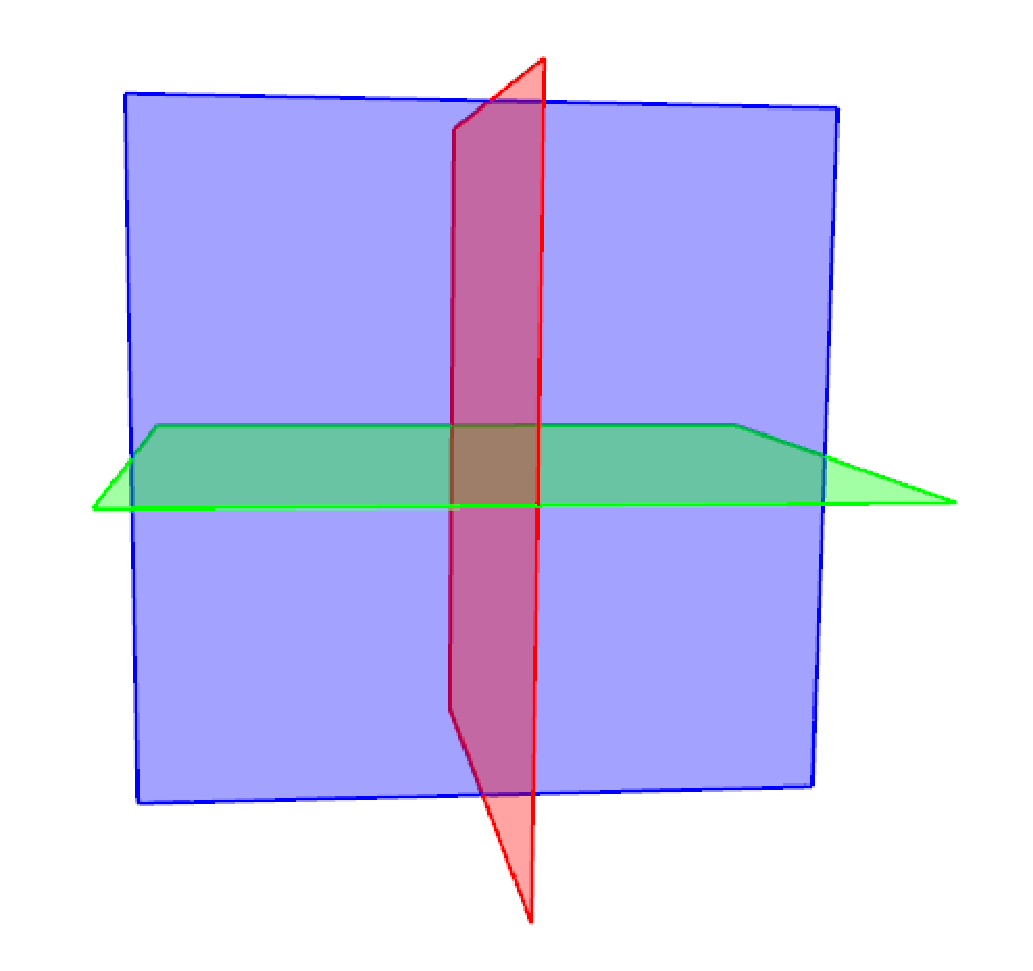
\includegraphics[scale=0.2]{figs/f3.pig-1.eps}
    \end{minipage}}
  \subfigure[]{
    \centering
    \label{fig:pig:b}
    \begin{minipage}[b]{0.18\textwidth}
      \centering
      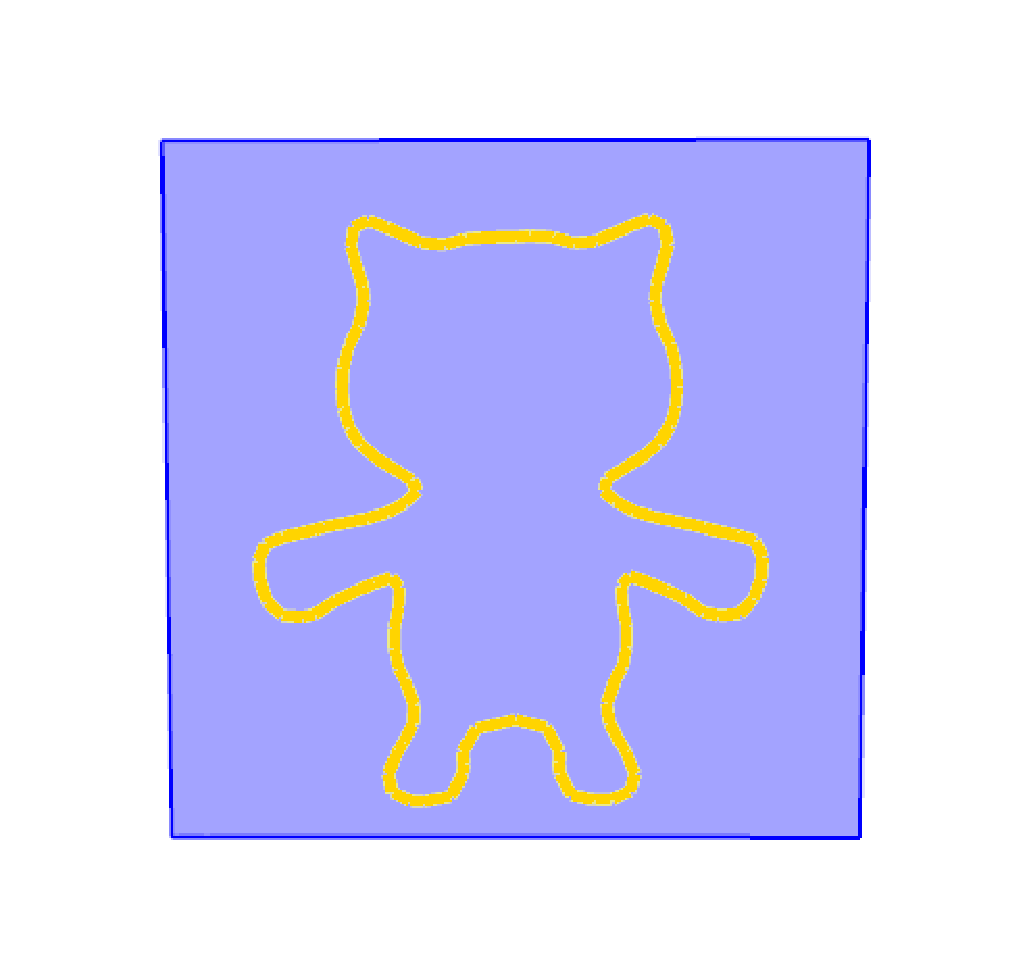
\includegraphics[scale=0.2]{figs/f3.pig-2.eps}
    \end{minipage}}
  \subfigure[]{
    \centering
    \label{fig:pig:c}
    \begin{minipage}[b]{0.18\textwidth}
      \centering
      
\includegraphics[scale=0.2]{figs/f3.pig-3.eps}
    \end{minipage}}
  \subfigure[]{
    \label{fig:pig:d}
    \begin{minipage}[b]{0.18\textwidth}
      \centering
      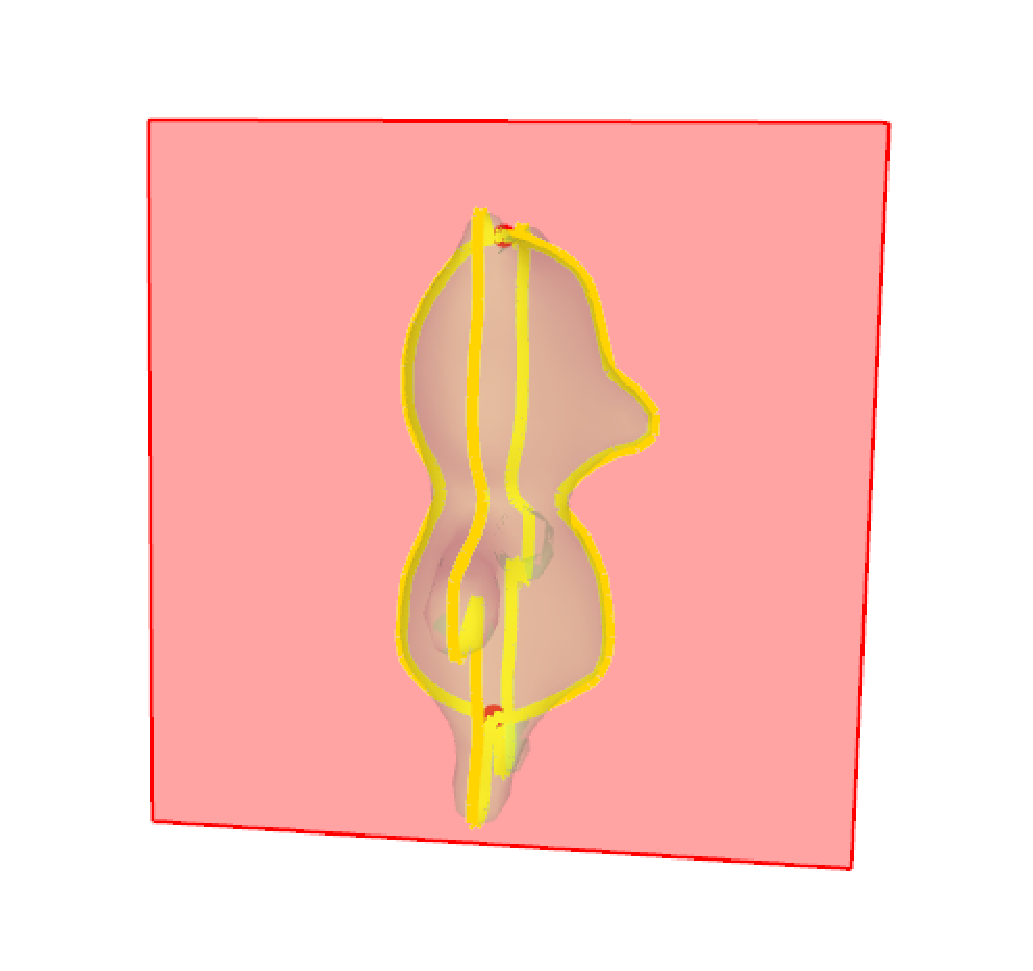
\includegraphics[scale=0.2]{figs/f3.pig-4.eps}
    \end{minipage}}
  \subfigure[]{
    \label{fig:pig:e}
    \begin{minipage}[b]{0.18\textwidth}
      \centering
      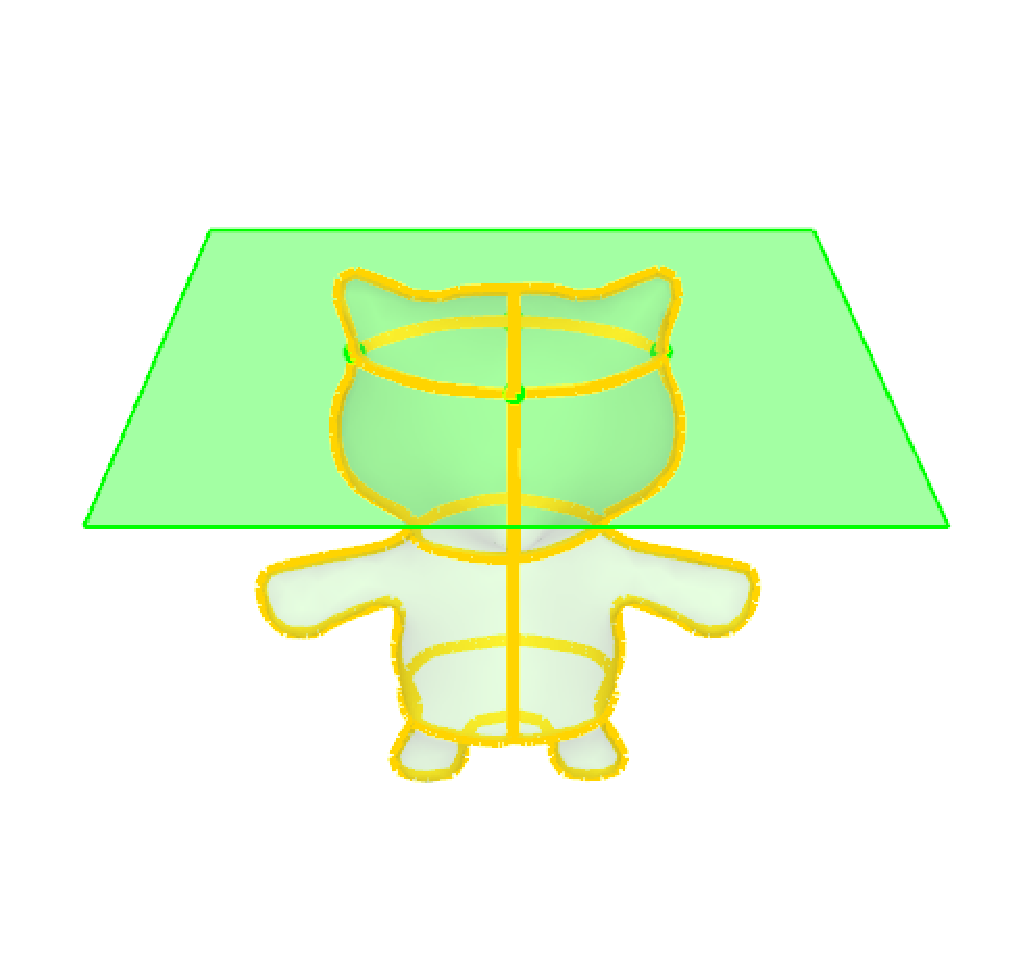
\includegraphics[scale=0.2]{figs/f3.pig-5.eps}
    \end{minipage}}
  \subfigure[]{
    \label{fig:pig:f}
    \begin{minipage}[b]{0.22\textwidth}
      \centering
      
\includegraphics[scale=0.22]{figs/f3.pig-6.eps}
    \end{minipage}}
  \subfigure[]{
    \label{fig:pig:g}
    \begin{minipage}[b]{0.22\textwidth}
      \centering
      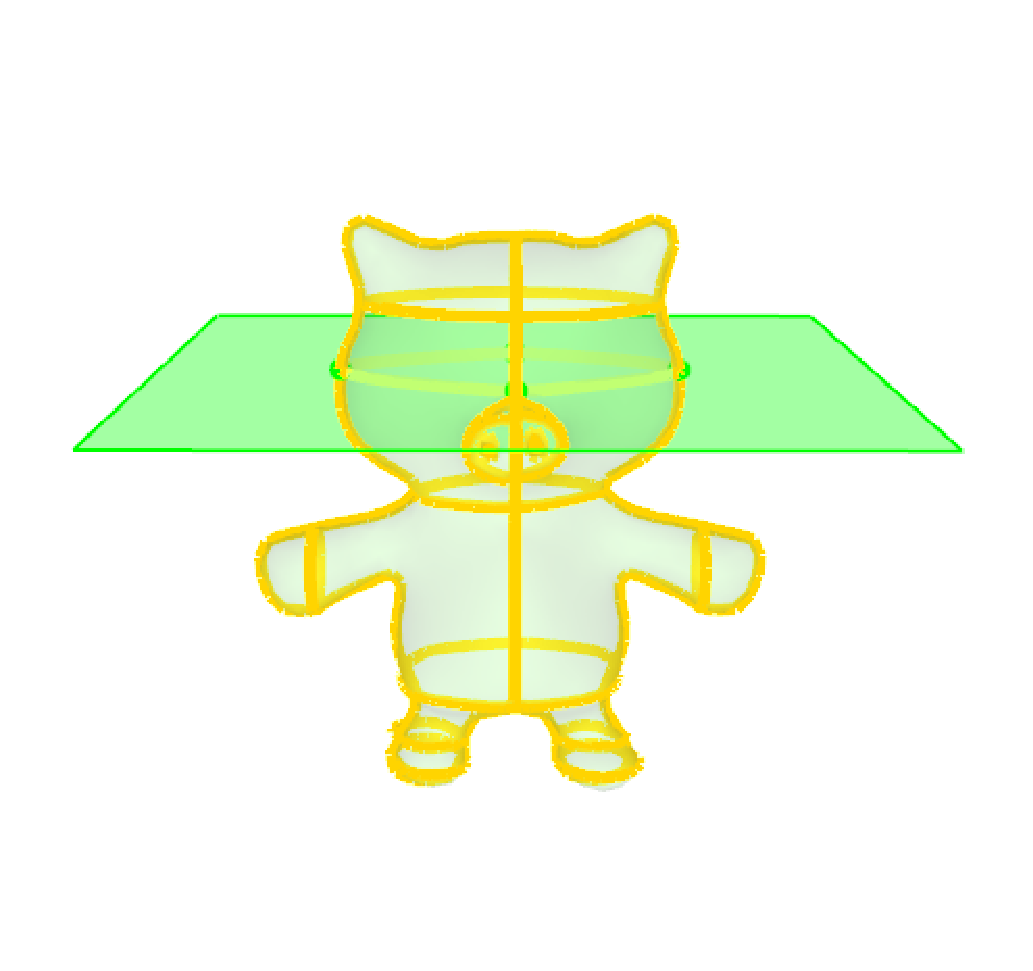
\includegraphics[scale=0.22]{figs/f3.pig-7.eps}
    \end{minipage}}
  \subfigure[]{
    \label{fig:pig:h}
    \begin{minipage}[b]{0.22\textwidth}
      \centering
      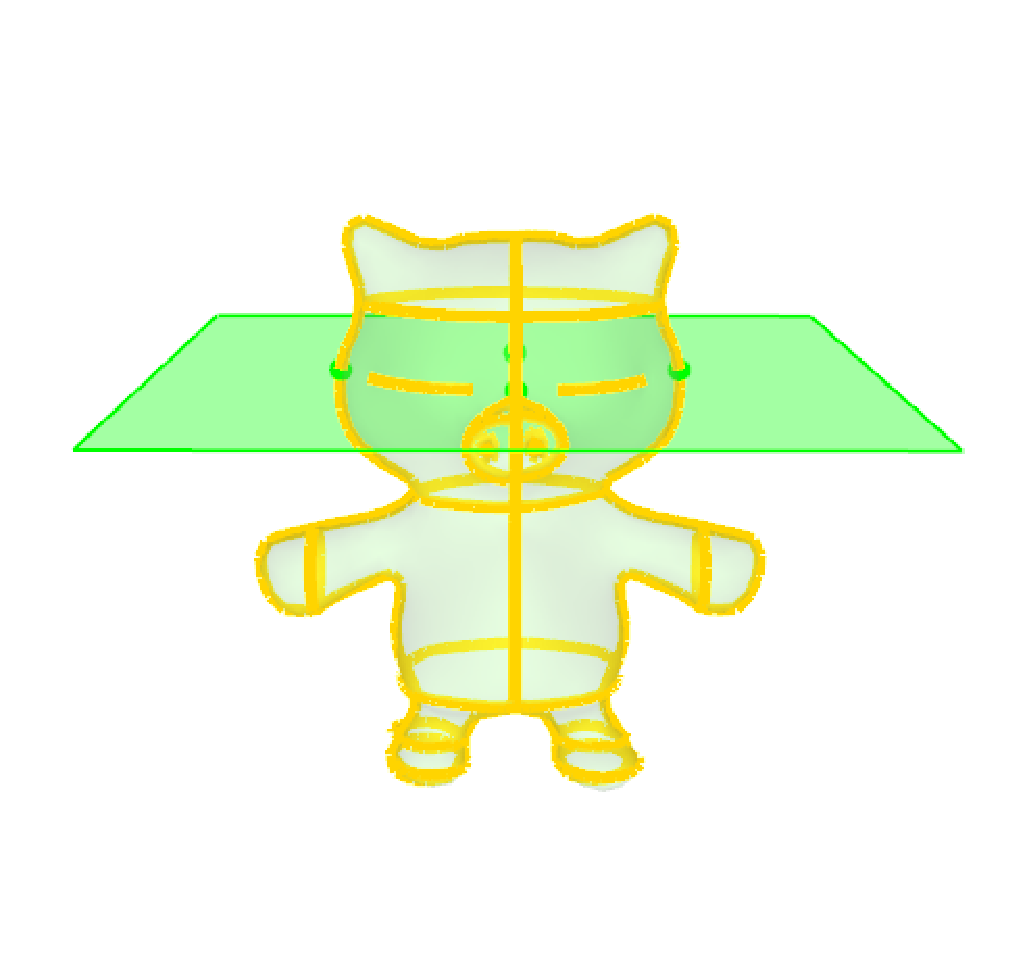
\includegraphics[scale=0.22]{figs/f3.pig-8.eps}
    \end{minipage}}
  \subfigure[]{
    \label{fig:pig:i}
    \begin{minipage}[b]{0.26\textwidth}
      \centering
      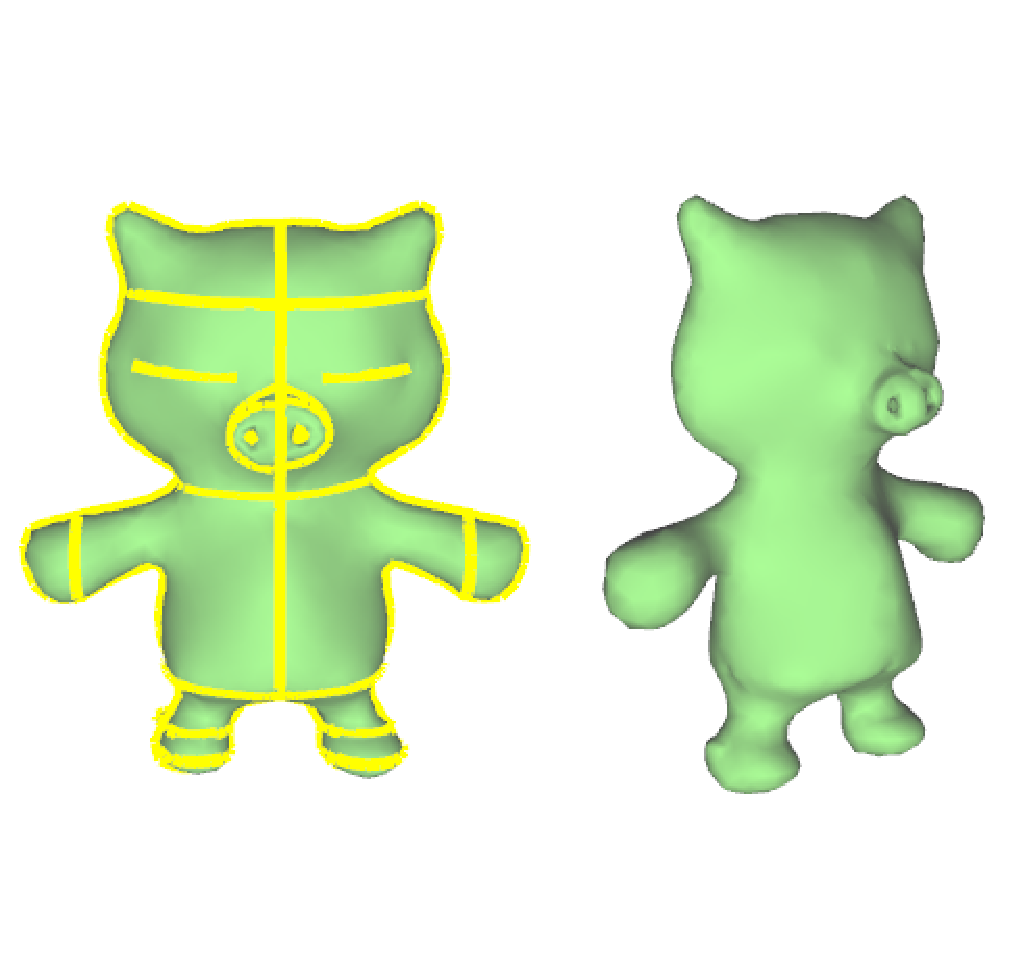
\includegraphics[scale=0.22]{figs/f3.pig-9.eps}
    \end{minipage}}
  \caption{Sketching tool. (a) Initially, three basic planes are provided; (b) A closed curve is sketched on the blue plane; (c) The preview of the reconstructed shape; (d) A new cross section is added on the red plane and the previewed shape is rendered; (e) The green plane is translated and three more cross sections are sketched; (f) More cross sections are added to refine the model; (g) The calculated cross section on the green plane is rendered semi-transparently to provide the user reference for further sketches; (h) Two incomplete cross sections are sketched on the green plane and the shape of the model is refined; (i) Final model.}
  \label{fig:pig} %% label for entire figure
\end{figure*}

%input of the system: cross sections on reference planes, why cross section
Our sketching tool provides the user three sets of orthogonal planes
as reference  planes. These reference planes are sketch planes, on
which the user can sketch the cross sections of the model. The word
\textit{cross section} means the intersection curve of the model
surface with a plane. We choose the cross section as the input of
the sketching tool for two considerations. First, it is an intuitive
and accurate description of a 3D model since it just lies on the
surface of the model. Comparing to other kinds of shape descriptors,
such as the silhouettes, it will cause less perception ambiguities
when the shape becomes complex. Second, a cross section is a planar
curve which can be quickly sketched in 3D space with the help of the
reference planes, and the sketching is thus simple yet effective for
depicting the 3D model. Meanwhile, taking the cross sections as the input
is also consistent with one of the visual rules in~\cite{HD00} that smooth
lines are usually interpreted as the contours of the 3D objects by human being.

%introduce reference planes
Initially, the $x=0$, $y=0$ and $z=0$ planes serve as the three
basic orthogonal planes. The user can define the cross sections of a
3D model by sketching strokes on any of these basic planes. These
three basic planes can also be translated along $x$, $y$ and $z$
axis respectively to allow the sketch of more contour curves. This
can result in several sets of parallel cross sections. Note that
though it is possible to rotate the basic planes to provide more
general reference planes and this could give the user more
flexibilities to sketch the contours, the price for this flexibility
is the algorithmic complexity of constructing 3D models from
non-parallel curve networks, the complexity of design and use of
interface, and the increase of occurrence of various ambiguities
from sketching. Therefore after a careful trade-off, we just allow
the basic planes to be translated and we find that this is generally
sufficient in practice for sketch-based freeform design.

%preview function, progresive modeling
The most distinguished feature of our system is the progressive
modeling function during sketching. That is, after the sketching on
one plane, the previewed up-to-date model which interpolates the
sketched strokes will be reconstructed and shown to the user. Since
comparing to the sculpting technique, sketching is an indirect way
of communicating with a shape, and it relies on the sense of human
perception~\cite{CIW08}, providing the previewed reconstruction
result can help the user to get a clear mind of the shape and
relative proportions of the constructed model after each sketch. It
also serves as a hint and reference on the following sketches and
makes the final shape conform to the user's expectation as much as
possible. Both the previewed model and the auxiliary planes are
rendered semi-transparently to avoid blocking the user's view on
existing sketches and the whole 3D space when providing sketching
references.

%auxiliary functions: operations on cross sections, highlighted intersection points, automatic view rotation
During the sketching process, all cross sections that  the user
sketched, as well as those calculated from the previewed model and
reference planes, are displayed and can be modified through
oversketching or deleted. Note that sketching cross sections on a
plane that intersects with the previewed shape looks similar to the
method adopted in~\cite{NSAC05,KSV09} at first glance, which shapes
a 3D model by iteratively oversketching its silhouette and deforming
it. However, the intrinsic difference lies in that the previewed
shape in our approach provides a reference for the following
sketches but sets little limitation on them, which means that these
sketches can be very flexible and the topology of the current shape
may even be changed. While in the deformation method the sketches
are restricted by the 3D model to be correspondence with the
existing cross sections on it, thus only the geometry of the current
shape can be modified.

%partial cross section
Since forcing the user to sketch complete cross sections may be
troublesome and inaccurate, we also allow the input to be just a
part of the cross section. Of course, such a stroke is to some
extent arbitrary and may not be explained as a valid part of the
cross section of the model to create. We thus set some requirements
for such an input and try to make it valid (see the details in
Section~\ref{ch4:sec:disc}).

%automatic view rotation
The system is also able to automatically rotate the view to make
the user selected plane for sketching face him as much as possible.
This is inspired by the observation in~\cite{BBS08} that a good view
for the user to sketch the 2D strokes is the one that has a large
visible projection. With this function, frequent manual viewpoint
changes which may interrupt the user's attention on the sketching
can be avoided.

%example
Figure~\ref{fig:pig} shows an overview of the creation process. With
 help of the reference planes and shapes, more descriptions on the
shape of a model can be sketched and perception ambiguities can be
reduced. This minimizes the unnecessary back and forth adjustment of
the sketches and speeds up the production process of a 3D model.

%cad system --> our system
It is noticed that our interface is similar to that in traditional
3D modeling software which provides the user three orthogonal views
to implement the modeling operations. This will make it easy to use
for users who are familiar with this type of interface. Moreover,
comparing to the system in~\cite{RDI10} which lets the user  sketch
the silhouettes of a 3D model on three orthogonal views, we give the
user the freedom to input more shape descriptions in 3D space, such
that less imagination will be needed when creating a 3D model with
multiple components and different depths.

%ambiguity and stroke rules
It should be pointed out that even though references have been
provided for defining the shape of a model, sometimes ambiguity
still occurs. The ambiguity arises from two aspects: the user input
strokes may not necessarily follow the same style -- different users
may have different manners for defining the shape of a model; even
with the same contours, the understandings of the shape they defined
may vary among different users. So some rules must be provided for
sketching the cross sections. The details of the rules will be
discussed in Section~\ref{ch3:sec:algo:rule}.

%-------------------------------------------------------------------------
\subsection{Sculpting tool}
\label{ch3:sec:ui:sculpt}

%sculpting functions
After the user sketches the general shape of the  model, we provide
a series of sculpting functions for him/her to do further
refinement. The sculpting tools include deformation, extrusion,
tunneling (digging a hole), cutting and smoothing functions, all of
which are based on the user's sketches. An intelligent stroke
recognition mechanism is used to judge the user's intention
according to the sketches and switch to the corresponding mode
automatically.

\subsubsection{Basic functions}
\label{Sec:UI:sculpt:mode}

\begin{figure} [htbp]
  \centering
  \subfigure[]{
    \centering
    \label{fig:sculpt:create} %% label for first subfigure
    \begin{minipage}[b]{0.45\textwidth}%0.45
      \centering
      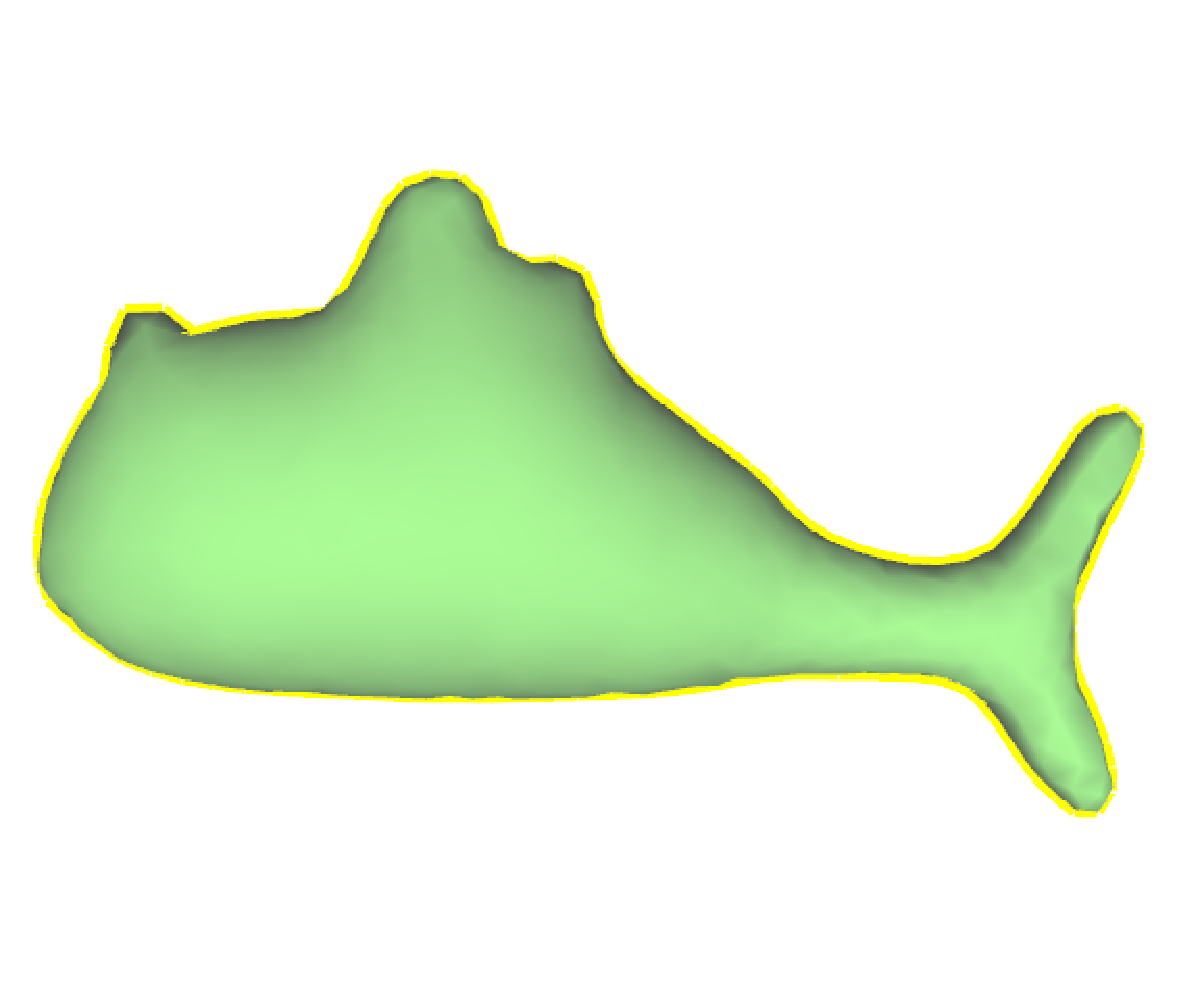
\includegraphics[scale=0.11]{figs/f3.fish-sculpt-1.eps}%0.12
    \end{minipage}}
   \subfigure[]{
    \centering
    \label{fig:sculpt:tunnel} %% label for first subfigure
    \begin{minipage}[b]{0.51\textwidth}%0.45
      \centering
      \includegraphics[scale=0.11]{figs/f3.fish-sculpt-2.eps}%0.1
    \end{minipage}}
   \subfigure[]{
    \centering
    \label{fig:sculpt:extrude} %% label for first subfigure
    \begin{minipage}[b]{0.48\textwidth}%0.38
      \centering
      \includegraphics[scale=0.11]{figs/f3.fish-sculpt-3.eps}%0.11
    \end{minipage}}
   \subfigure[]{
    \centering
    \label{fig:sculpt:cut} %% label for first subfigure
    \begin{minipage}[b]{0.48\textwidth}%0.5
      \centering
      \includegraphics[scale=0.11]{figs/f3.fish-sculpt-4.eps}%0.11
    \end{minipage}}
   \subfigure[]{
    \centering
    \label{fig:sculpt:smooth} %% label for first subfigure
    \begin{minipage}[b]{0.9\textwidth}%0.38
      \centering
      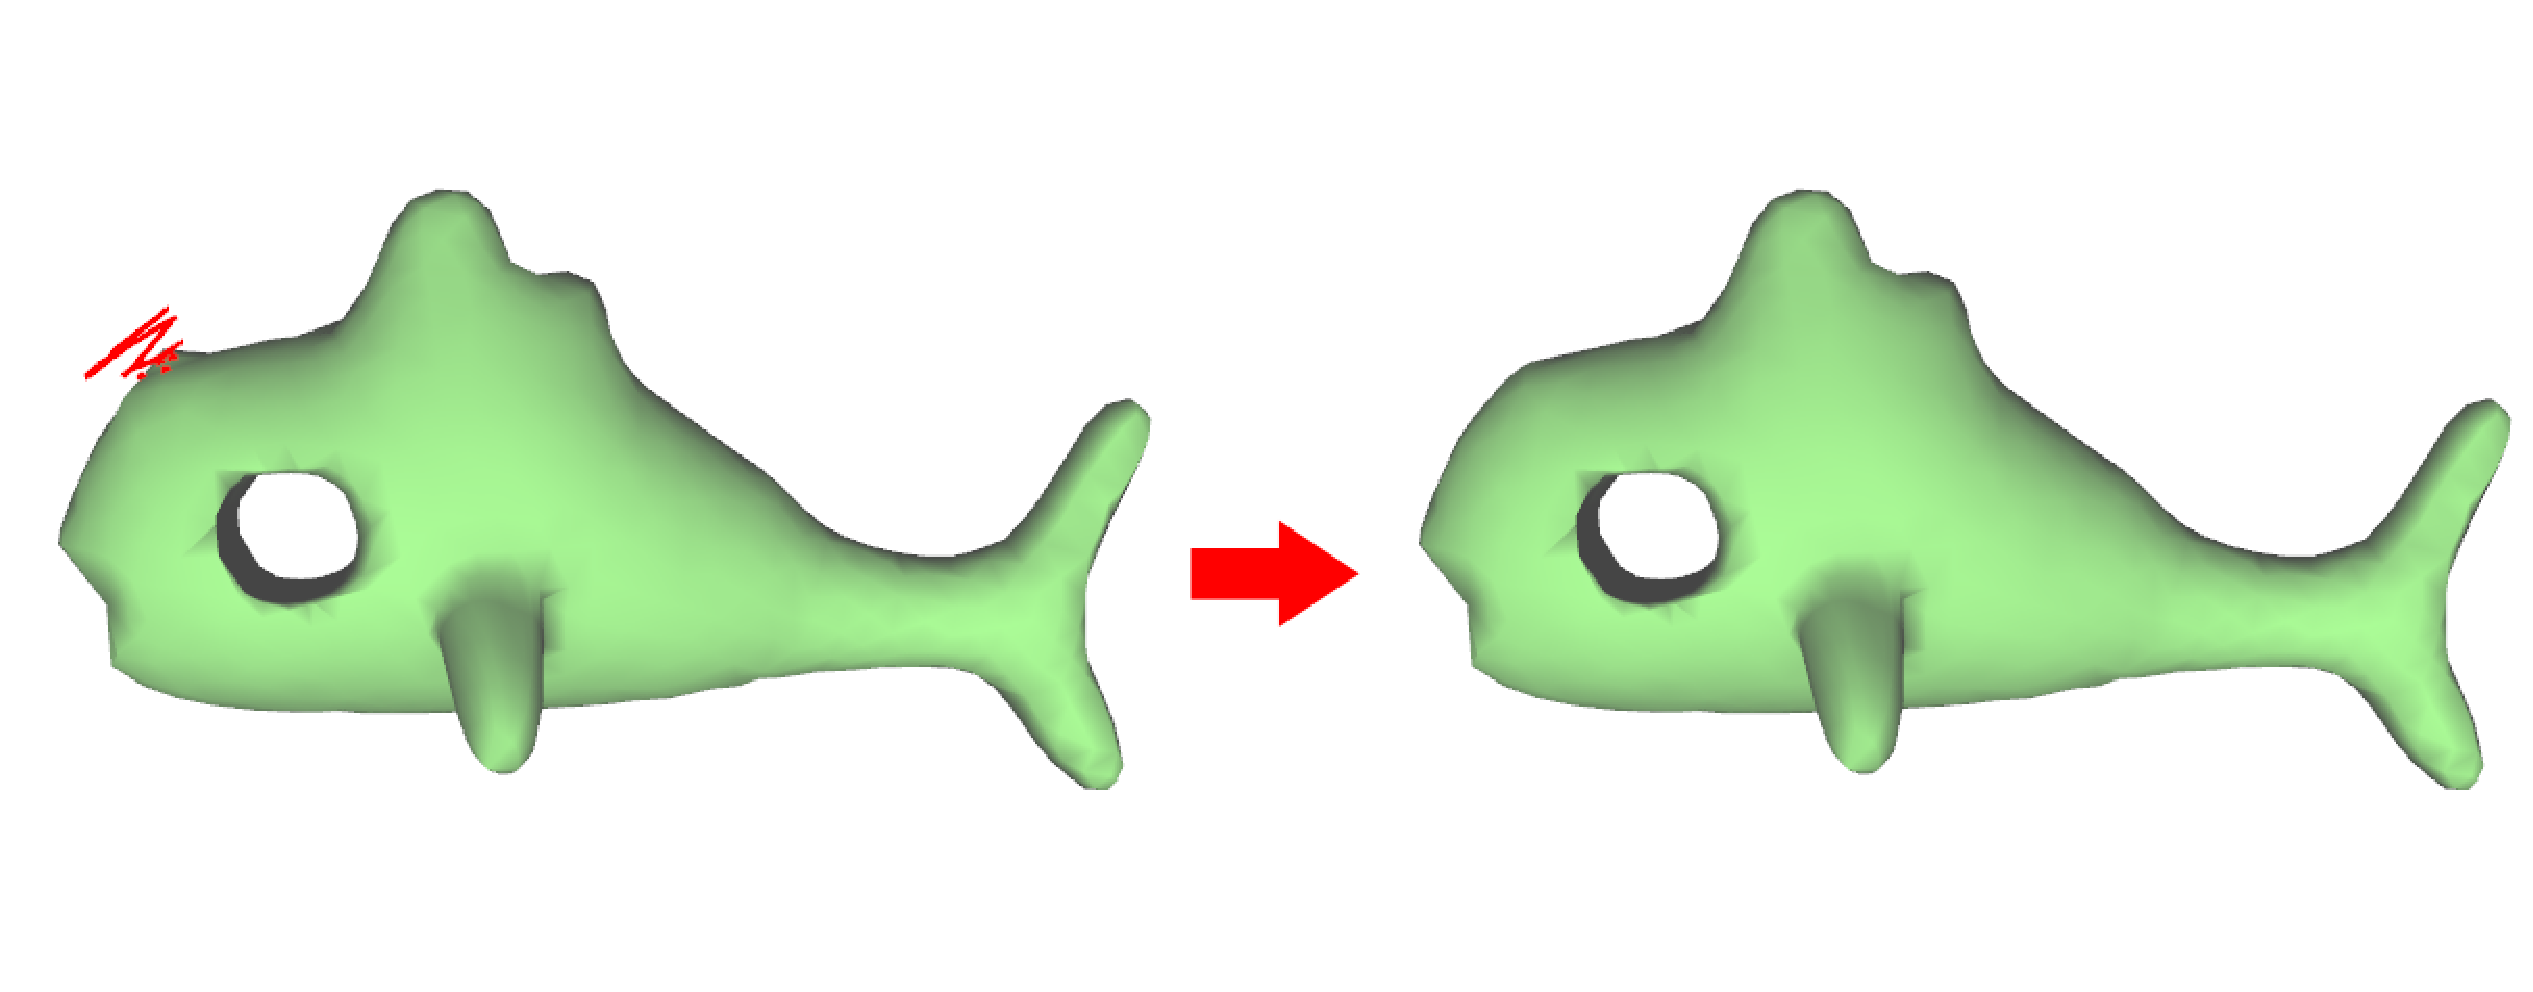
\includegraphics[scale=0.11]{figs/f3.fish-sculpt-5.eps}%0.11
    \end{minipage}}
  \caption{Sculpting tools. (a) The user sketched cross section (yellow) and initially generated model; (b) Tunneling operation; (c) Extrusion operation; (d) Cutting operation; (e) Smoothing operation.}
  \label{fig:sculpt} %% label for entire figure
\end{figure}

%stroke types. open stroke
The stroke set our system accepts in the sculpting tool includes
three general types: a simple open stroke, a closed stroke, and a
scratch-out stroke. When a simple open stroke is sketched, the
operation may be cutting or deformation, depending on whether the
stroke passes across the model in the image space or not. If it is a
cutting stroke, a following stroke will be required to indicate
which part to cut off (Figure~\ref{fig:sculpt:cut}). The subsequent
operation of deformation will be introduced in detail in
Section~\ref{ch3:sec:ui:sculpt:deform}.

%closed strokes, extrusion or tunneling
We allow the user to extrude or dig  a part similar to the operation
in~\cite{IMT99,NISA07} when a closed stroke is sketched on the
surface of the model. What is different, our system automatically
generates a reference plane orthogonal to the closed curve, on which
the user can draw the silhouette curve of the extruded/dug part
(Figure~\ref{fig:sculpt:extrude}). This plane can be rotated about
two axes: the line passing through the center of the closed stroke
and orthogonal to the stroke as much as possible or the line
connecting the first drawn point of the closed stroke and the
farthest point to it on the stroke. The reference plane helps to
confirm the position of the silhouette curve and gives flexibility
to adjust its direction. When the silhouette curve intersects with
the backside surface, the operation turns to tunneling and a hole is
dug (Figure~\ref{fig:sculpt:tunnel}).

%scratch strokes, smoothing
When the user scratches a part on the model back and  forth, it is
regarded as a smoothing operation and the local part will be
smoothed (Figure~\ref{fig:sculpt:smooth}).


\subsubsection{Deformation tool}
\label{ch3:sec:ui:sculpt:deform}

\begin{figure*} [htbp]
  \centering
  \subfigure[]{
    \centering
    \label{fig:deform:a} %% label for first subfigure
    \begin{minipage}[b]{0.3\textwidth}
      \centering
      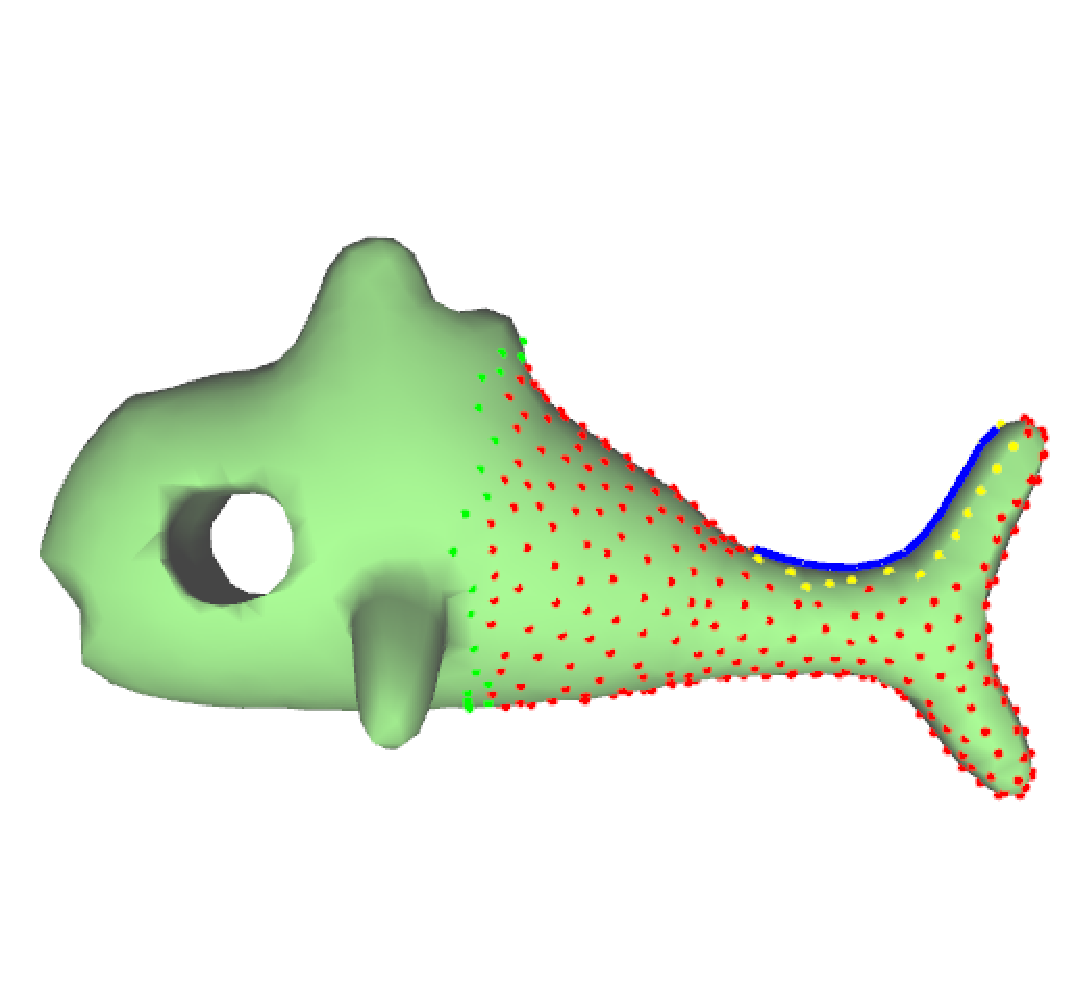
\includegraphics[scale=0.15]{figs/f3.fish-deform-1.eps}
    \end{minipage}}
  \subfigure[]{
    \centering
    \label{fig:deform:b}
    \begin{minipage}[b]{0.3\textwidth}
      \centering
      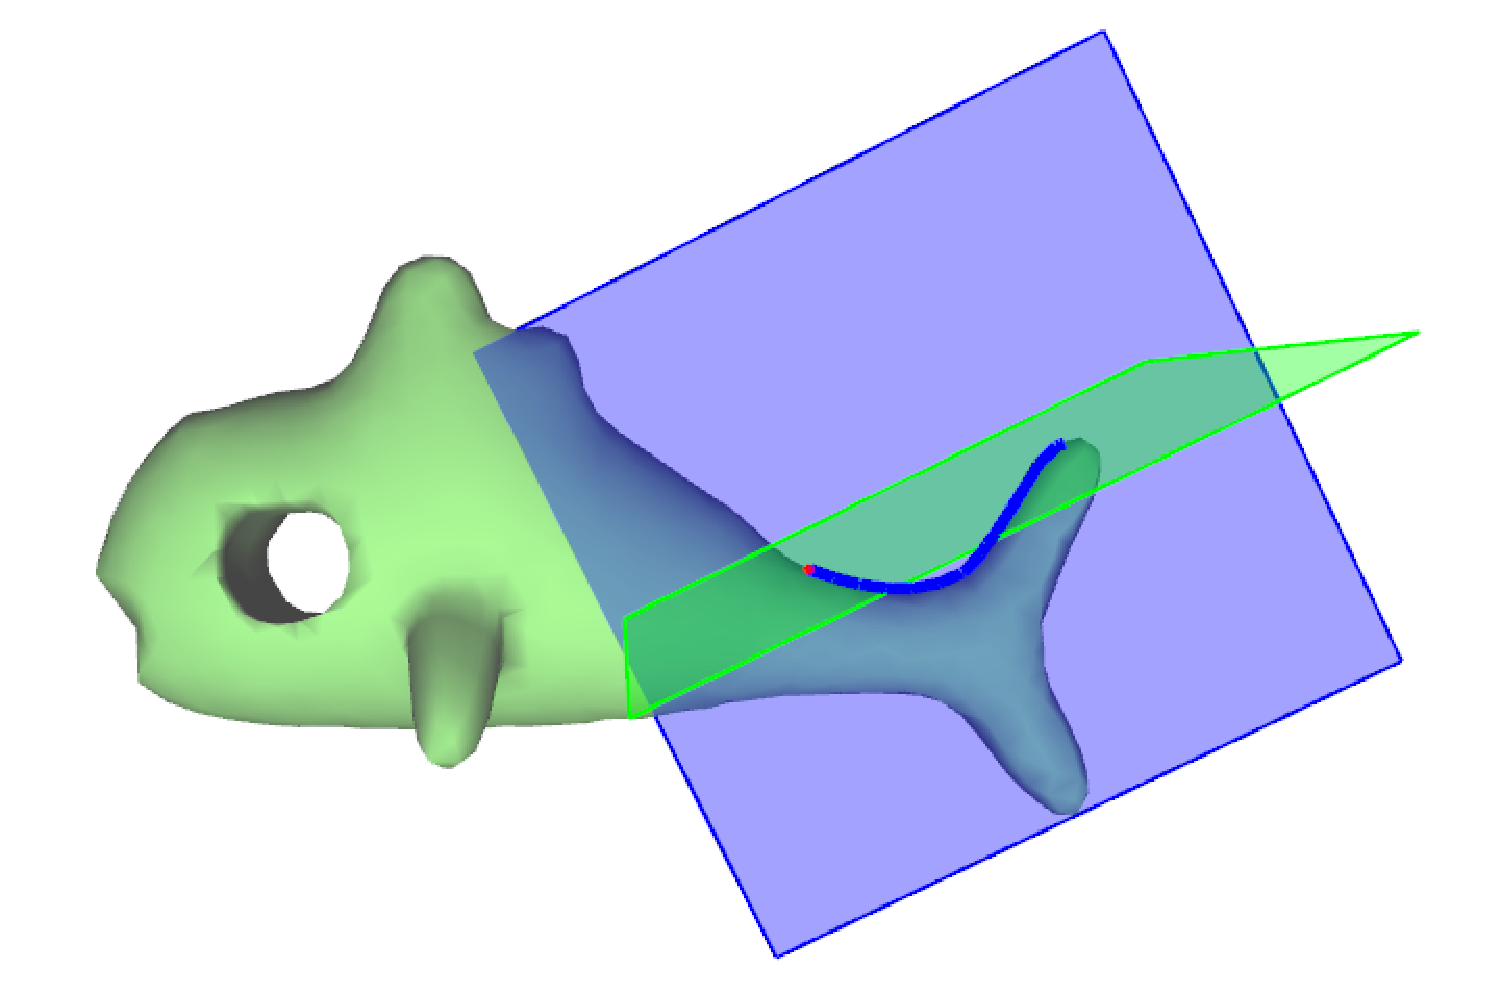
\includegraphics[scale=0.15]{figs/f3.fish-deform-2.eps}
    \end{minipage}}
  \subfigure[]{
    \centering
    \label{fig:deform:c}
    \begin{minipage}[b]{0.3\textwidth}
      \centering
      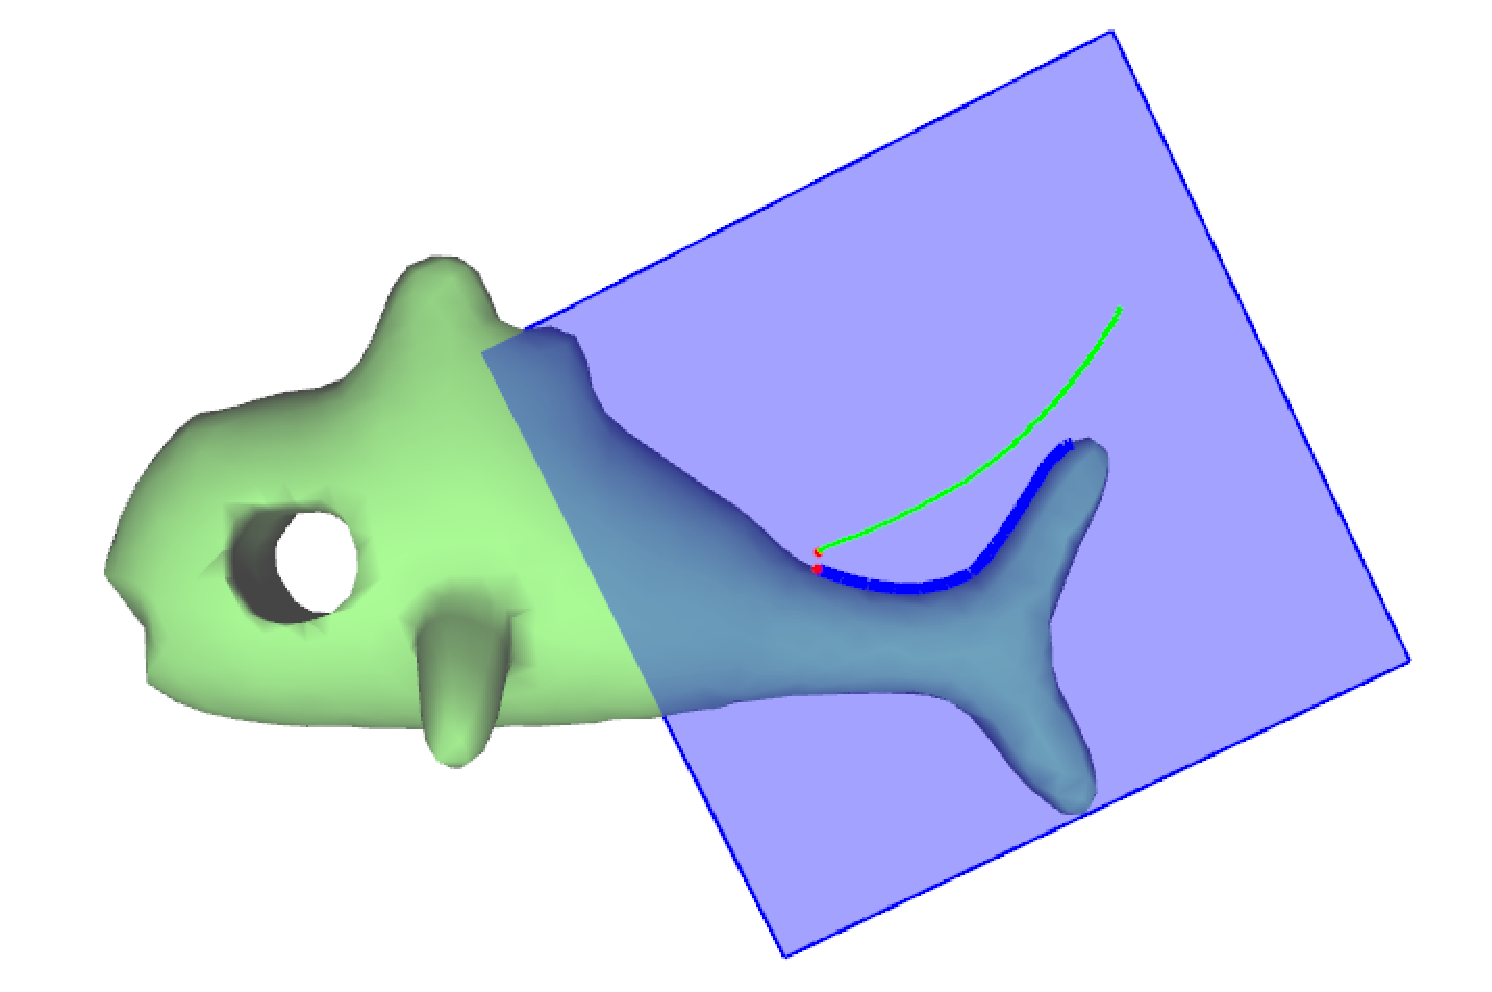
\includegraphics[scale=0.15]{figs/f3.fish-deform-3.eps}
    \end{minipage}}
  \subfigure[]{
    \label{fig:deform:d}
    \begin{minipage}[b]{0.3\textwidth}
      \centering
      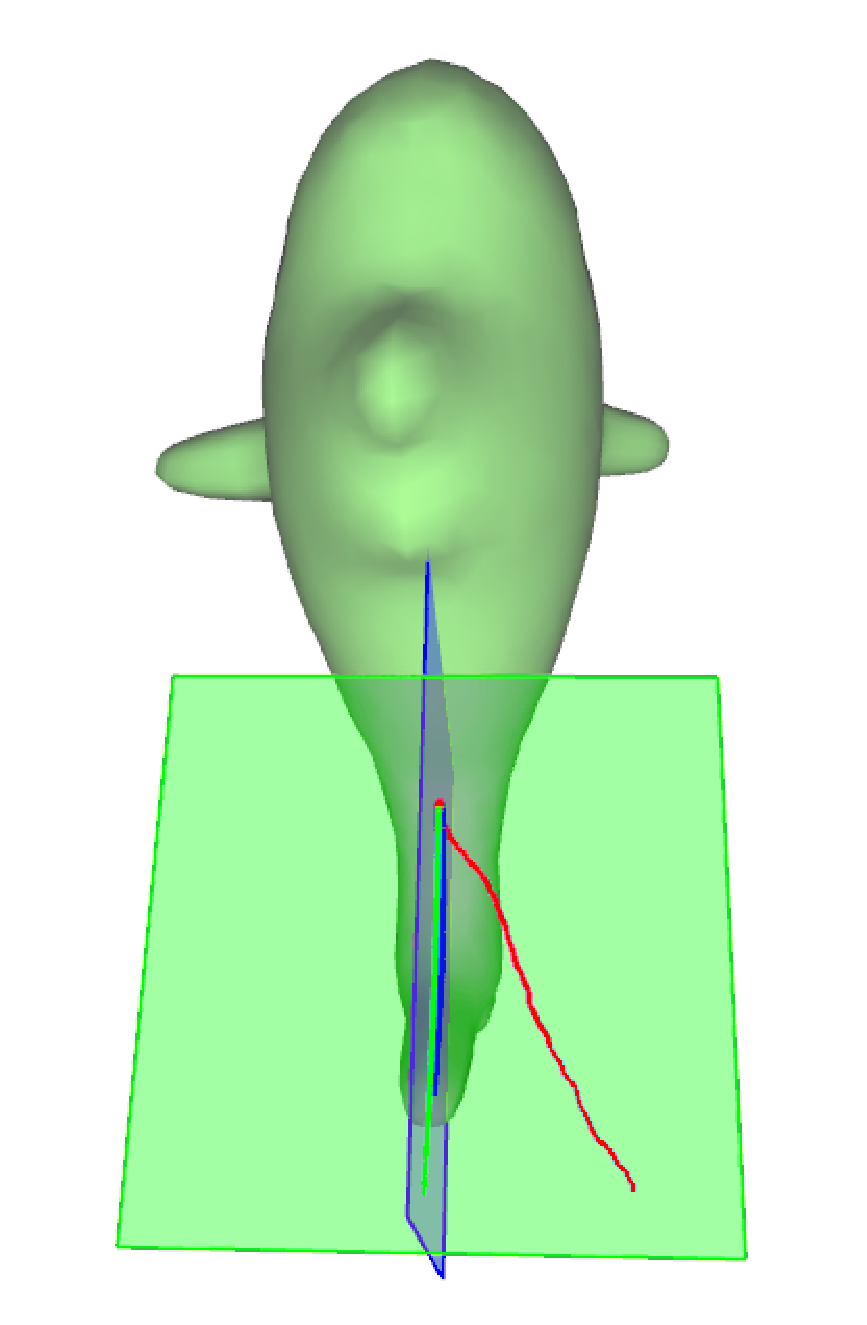
\includegraphics[scale=0.15]{figs/f3.fish-deform-4.eps}
    \end{minipage}}
  \subfigure[]{
    \label{fig:deform:e}
    \begin{minipage}[b]{0.3\textwidth}
      \centering
      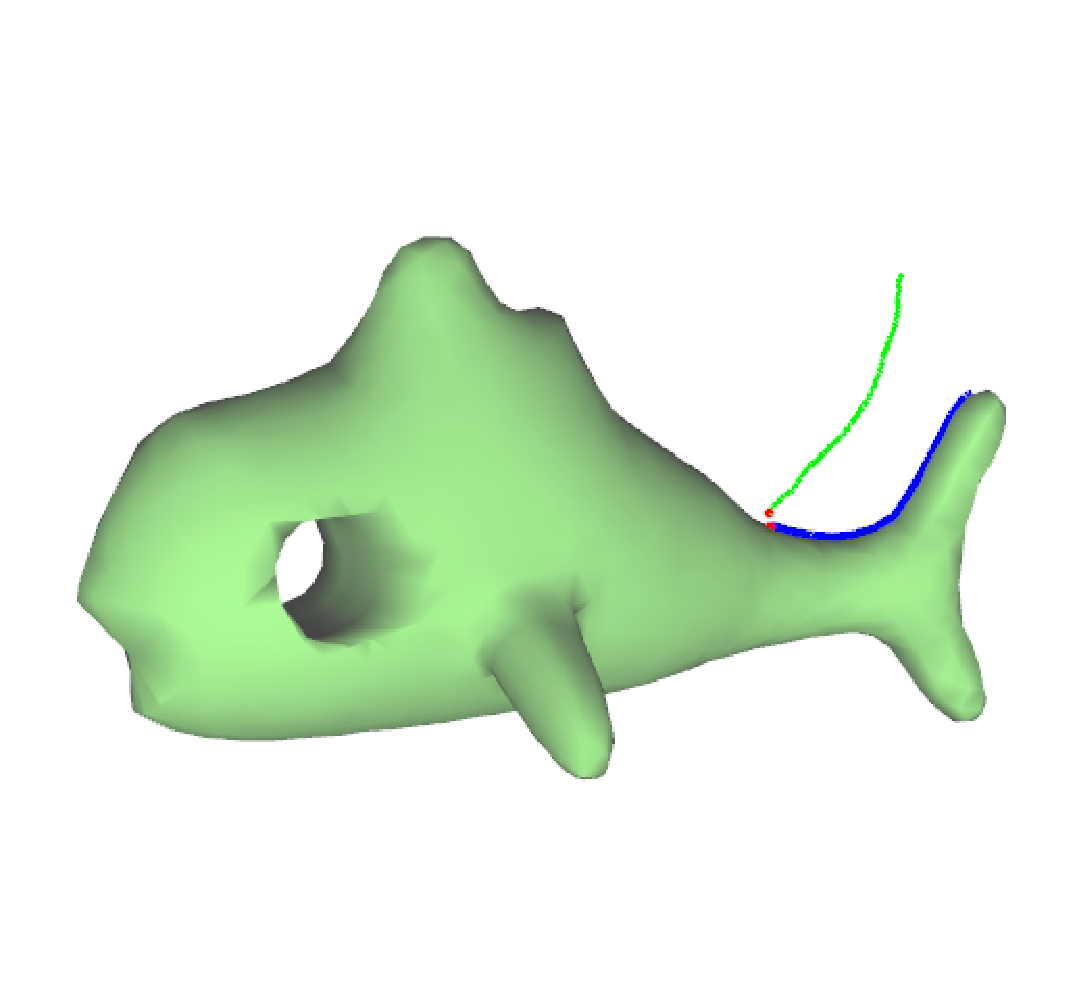
\includegraphics[scale=0.15]{figs/f3.fish-deform-5.eps}
    \end{minipage}}
  \subfigure[]{
    \label{fig:deform:f}
    \begin{minipage}[b]{0.3\textwidth}
      \centering
      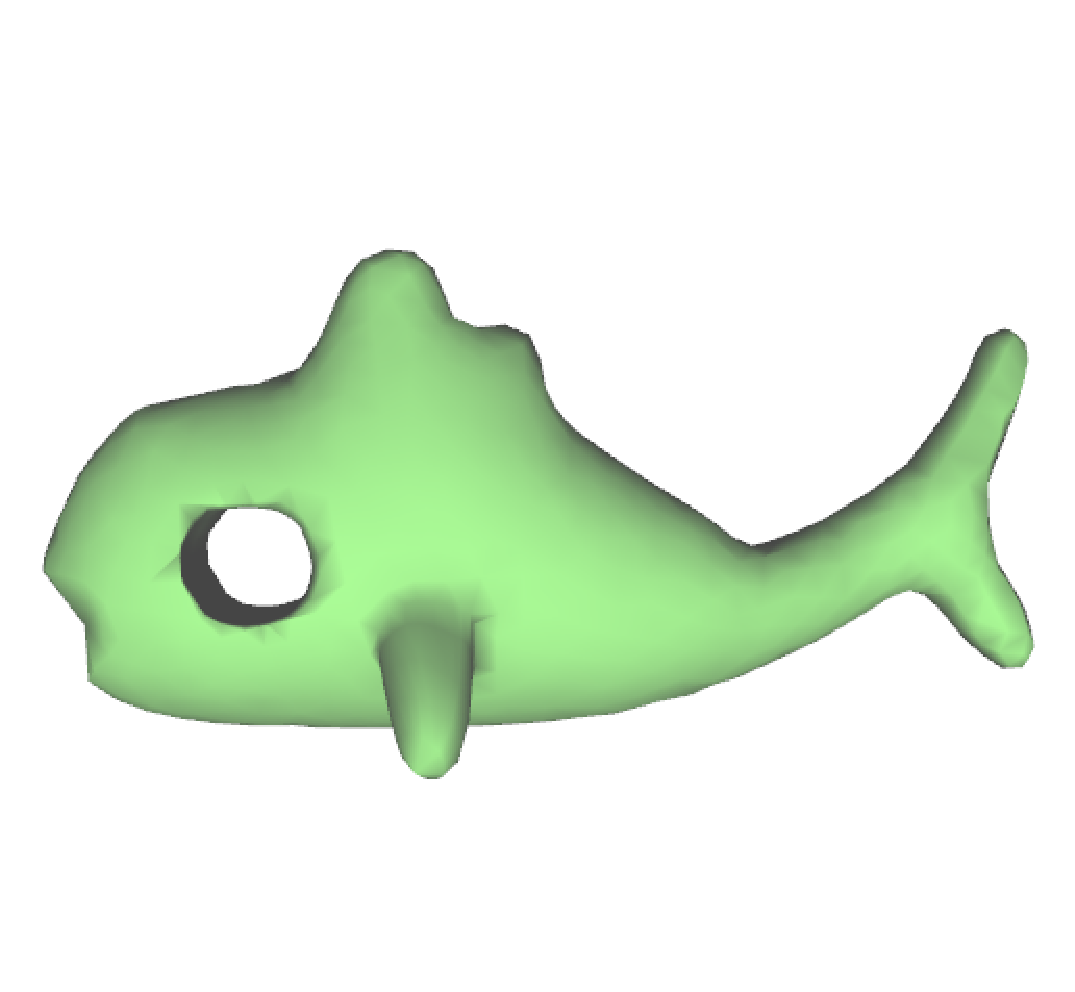
\includegraphics[scale=0.15]{figs/f3.fish-deform-6.eps}
    \end{minipage}}
  \caption{An example of using the deformation tool. (a) The blue curve is the handle curve sketched on the initial model. The yellow, red and green dots denote the handle, ROI and static vertices respectively; (b) The automatically generated base plane (blue) and projection plane (green); (c) The new curve (green) drawn on the base plane; (d) A curve (red) is drawn on the projection plane to create a non-planar new curve; (e) The updated new curve (green); (f) The deformed model.}
  \label{fig:deform} %% label for entire figure
\end{figure*}

%introduction of deformation, why handle curve instead of point
The deformation tool is an important  sculpting function in our
system. As introduced in Section~\ref{ch2:sec:sbim:sculpt}, to
deform a mesh, a handle needs to be first specified for the
following operations. Here we use a curve as the handle instead of a
point, since it contains multiple points and thus provides more
flexibility for the manipulation. The user needs to first sketch a
stroke which will be projected onto the mesh to generate the handle
curve. Two reference planes will then be generated automatically.
Next, the user needs to sketch on the reference planes to specify
the new shape and position of the handle curve, after which the
deformation is completed. To implement this deformation process, the
following information should be specified: a set of vertices (called
handle vertices) and their new positions; the vertices within a
region of interest (ROI), which will move with the handles; and the
vertices will remain unchanged during the deformation process
(called the static vertices).

%how to compute handle curve
To generate the handle curve, we use a method similar to that
in~\cite{NSAC05}. The handle curve is composed of handle vertices.
The vertices of the edges or faces on which the projection of the
input stroke lie are regarded as the handle vertices. See
Figure~\ref{fig:deform:a} for an illustration.

%new position of handle curve
The specification of new positions of the handle  vertices seems not
trivial. Unlike previous existing methods, we provide the user with
two reference planes for the sketching of the new curve: a base
plane which passes the handle vertices as many as possible for
sketching the basic shape of the new curve and a projection plane,
which is orthogonal to the base plane, for drawing the projection of
the new curve (Figure~\ref{fig:deform:b}). In general, the base
plane is sufficient for sketching the new shape of the handle curve.
However, if the new handle curve is desired to be non-planar, the
projection plane is used to sketch its projection and then the new
handle curve is determined (Figure~\ref{fig:deform:c} -
Figure~\ref{fig:deform:e}). In addition, in our system the two
planes can also be rotated to provide more flexibility. In this way,
the user can draw arbitrary curves in 3D space while being fully
aware of the locations.

%ROI vertices
For selection of the ROI vertices, three methods  are available. A
simple approach is to specify a threshold and vertices whose
Euclidean distances to the handles below this threshold are regarded
as the ROI vertices. Another approach is to let user draw a circle
on the 2D screen. The ROI vertices are the ones whose projections
onto the screen are inside the circle. However these two methods
seem not quite precise when the selection of certain vertices is
required for relatively complex models. So we provide a new tool --
a brush, to make the selection process somewhat like brushing on a
model. The vertices brushed will then be chosen as the ROI vertices.
The brush can be viewed as a complementary tool for the former two
methods. The user could take a rough selection using the first two
tools and then make further modifications by brushing on the model.

These sculpting tools are all sketch-based and quite convenient to
use. Together with the sketching tool, a complete modeling system is
built up. With this system, the user could easily create and edit a
3D object in a short period by sketching strokes.


%-------------------------------------------------------------------------
\section{Algorithms}
\label{ch3:sec:algo}

In this section we describe the underlying algorithms of the
sketching interface. We first introduce the preprocessing algorithm
for the input strokes. Then we propose the stroke rules for
interpreting input cross sections and making them valid for the
computation of the 3D model. Finally the  algorithm for the
calculation of the reference planes in the sculpting tool is
provided.

%-----------------------------------------------------------------------------------------------------------------
\subsection{Input stroke preprocessing}\label{ch3:sec:alg:strokepreproc}

For sketch-based modeling systems, the original input stroke created
from an input device usually cannot be used directly due to two
reasons: 1). The points of the stroke are noisy because of the shaky
nature of handling the input devices; 2). the spatial and temporal
quantization of the input by the hardware may contain error since
the speed that the user draws is random. Thus, we perform a
three-step preprocessing of the input stroke in each functions, as
shown in Figure~\ref{fig:alstrokeproc}.

\begin{figure} [htbp]
  \centering
  \subfigure[]{
    \centering
    \label{fig:alstrokeproc:a} %% label for first subfigure
    \begin{minipage}[b]{0.2\textwidth}
      \centering
      
\includegraphics[scale=0.3]{figs/f3.strokepre-1.eps}
    \end{minipage}}
  \subfigure[]{
    \centering
    \label{fig:alstrokeproc:b}
    \begin{minipage}[b]{0.2\textwidth}
      \centering
      
\includegraphics[scale=0.3]{figs/f3.strokepre-2.eps}
    \end{minipage}}
  \subfigure[]{
    \centering
    \label{fig:alstrokeproc:c}
    \begin{minipage}[b]{0.2\textwidth}
      \centering
      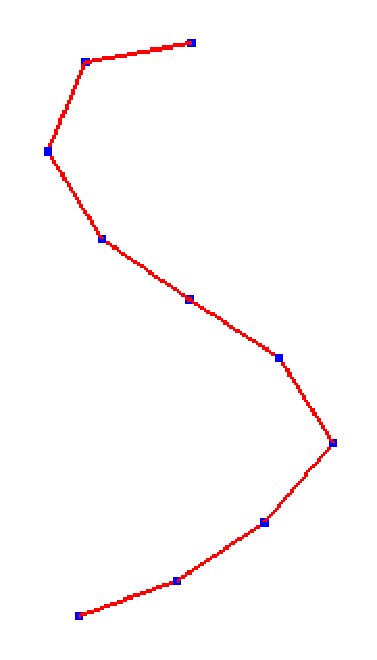
\includegraphics[scale=0.3]{figs/f3.strokepre-3.eps}
    \end{minipage}}
  \subfigure[]{
    \centering
    \label{fig:alstrokeproc:d}
    \begin{minipage}[b]{0.2\textwidth}
      \centering
      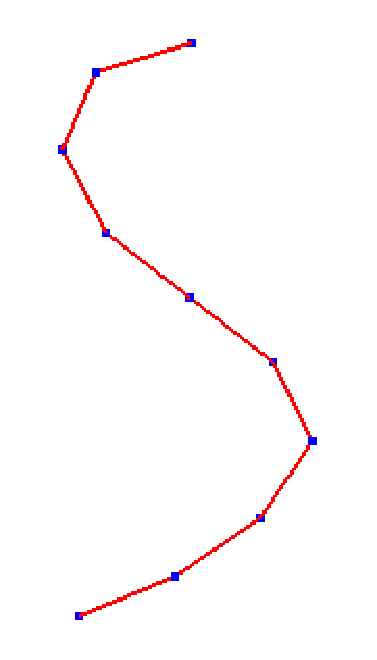
\includegraphics[scale=0.3]{figs/f3.strokepre-4.eps}
    \end{minipage}}
  \caption{Stroke Preprocessing: The goal here is to filter the noisy points and get a smooth curve with 10 points. (a) Initial input; (b) Filtering result; (c) Resampling result; (d) Final result after smoothing.}
  \label{fig:alstrokeproc} %% label for entire figure
\end{figure}

First of all, a point whose distance to its previous one is less
than a given threshold will be judged as a redundant noisy point and
deleted.

Then we resample the stroke to make its points number a  predefined
value $N_{pre}$. To do this, we first calculate the summed distance
$S_{total}$ between each two points to get the length of the stroke.
Then through dividing $S_{total}$ by $N_{pre}$, we get the expected
unit distance $S_{unit}=S_{total} / N_{pre}$ along the route of the
stroke between each two new points. Finally starting from the first
point, we \lq\lq{travel}\rq\rq along the original stroke trajectory.
Every time when a unit distance $S_{unit}$ reaches, we position a
new stroke point. The \lq\lq{journey}\rq\rq ends until the last new
point is placed. A new curve is then formed.

This simple resampling algorithm can produce a stroke with a desired
number of points. The original shape of the stroke is preserved as
much as possible. Meanwhile, it is quite easy to implement and
avoids complicated computations required in some existing methods
(for example, fitting a polyline to a B-spline and evenly sample
it~\cite{CMZHB99}).

Finally the stroke is smoothed by moving each point according to Eq.~\ref{eq:strokesmooth}.

\begin{equation}
\label{eq:strokesmooth}
    P_i^\prime = \frac{P_{i-1}+4*P_i+P_{i+1}}{6}
\end{equation}
where $P_i$ and $P_i^\prime$ are the old and new positions of point
$i$. $P_{i-1}$ and $P_{i+1}$ are the old positions of its two
neighbor points.

The stroke preprocessing is a fundamental step for the functions in
the system and helps to produce a visually-pleasant 3D model.


\subsection{Stroke rules}
\label{ch3:sec:algo:rule}

As mentioned in Section~\ref{Sec:UI:sketch}, to avoid the
perception ambiguity, some rules are needed to regularize and
interpret the user sketched strokes before we construct the surface.
It is suggested in the guidelines for the user interface design
in~\cite{MN90} that the interface should match with the real world
conventions, which is coincident with the user psychology that the
user always prefer familiar concepts rather than system-oriented
terms~\cite{GC87,DA06}. Thus, these stroke rules should make the
input curves consistent with the common sense of the cross sections
which represent the intersections of the planes and the surface
of a 3D object with no self-intersections. Specifically, these
rules include:

\begin{enumerate}
    \item For curves on a plane, if they do not intersect with or contain each other, the interior of each curve belongs to the interior of the model.
    \label{rule:1}
    \item For two curves $S_1$ and $S_2$ on a plane, if $S_1$ is totally contained in $S_2$, then it means that the intersection between the plane and the model is a ring. If the containing relationship exists among more than two curves, that is, we have $n$ curves $S_1,S_2,...,S_n$ and $S_i$ is within $S_{i+1}$, then we start the perception from the outermost pair of curves $S_n$ and $S_{n-1}$.
    \label{rule:2}
    \item If a curve is self-intersected or intersects with any other curves lying on the same plane, then it is treated as an invalid curve and thus discarded.
    \label{rule:3}
    \item For two curves $S_1$ and $S_2$ lying on two orthogonal planes $P_1$ and $P_2$ respectively, the intersection point set $\{V_{S_1P_2}\}$ of curve $S_1$ and plane $P_2$, must be exactly the \emph{same} as the set $\{V_{S_2P_1}\}$ of $S_2$ and plane $P_1$.
    \label{rule:4}
\end{enumerate}

Next we give some explanations of these rules.  The first rule is
easy to understand. When a user draws one or more closed strokes,
the strokes are usually regarded as the outer contours of an object.

When a user tries to make a hole on the mesh surface  to create a
relatively complex model, a pair of curves are often used, of which
one is contained in the other. The ring between the two curves is
the interior part of the model. If more holes are desired, more
pairs of curves should be used. To avoid the ambiguity of
perception, the order of analysis is inward starting from the
outermost pair. For example, suppose we have $n$ curves
$S_1,S_2,...,S_n$ and $S_{i-1}$ is totally contained in  $S_i$. Then
$S_n$ and $S_{n-1}$ form a ring, $S_{n-2}$ and $S_{n-3}$ form
another ring which is contained in the previous one, and so on. If
$n$ is an even number, then the ring formed by $S_2$ and $S_1$ is
innermost; Otherwise we just apply rule~\ref{rule:1} to $S_1$ -- the
interior of $S_1$ is the interior of the model. An example of
rule~\ref{rule:2} is shown in Figure~\ref{fig:rule2}.
Rule~\ref{rule:2} makes it possible to model a mesh with arbitrary
topology directly by sketching the contours at the creation phase.

\begin{figure} [htbp]
  \centering
  \subfigure[]{
    \centering
    \label{fig:rule2:a} %% label for first subfigure
    \begin{minipage}[b]{0.22\textwidth}
      \centering
      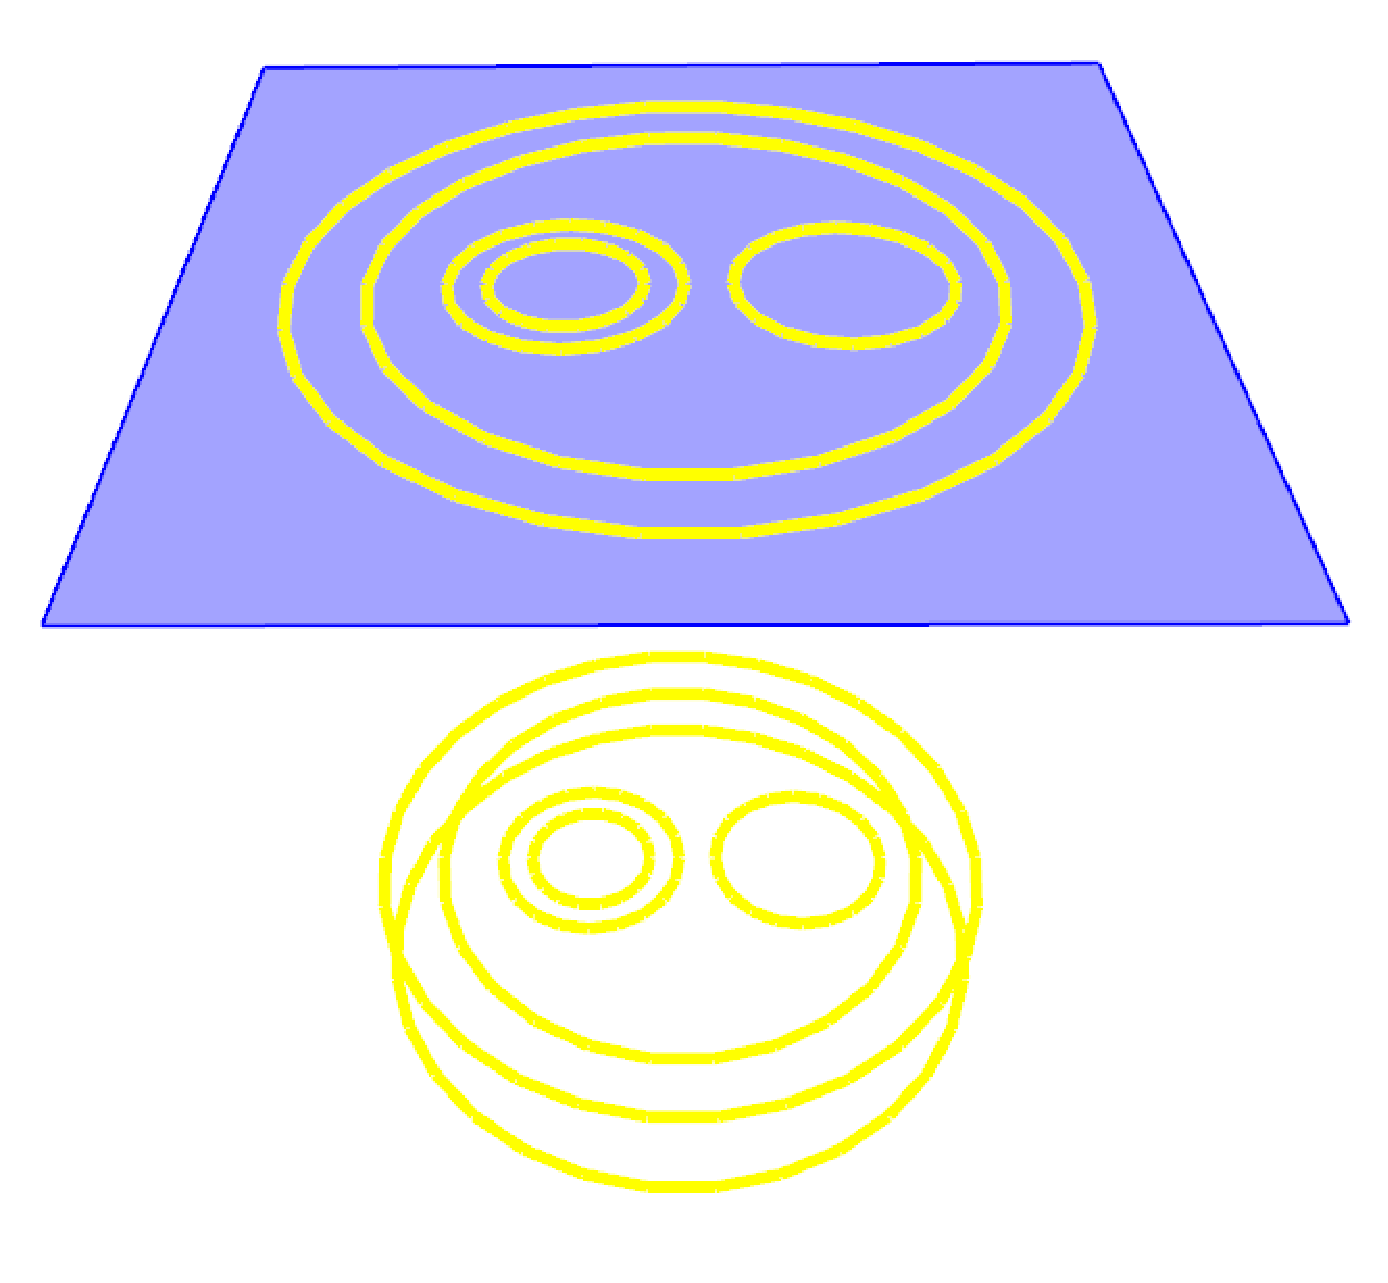
\includegraphics[scale=0.12]{figs/f3.rule2-1.eps}
    \end{minipage}}
  \subfigure[]{
    \centering
    \label{fig:rule2:b}
    \begin{minipage}[b]{0.22\textwidth}
      \centering
      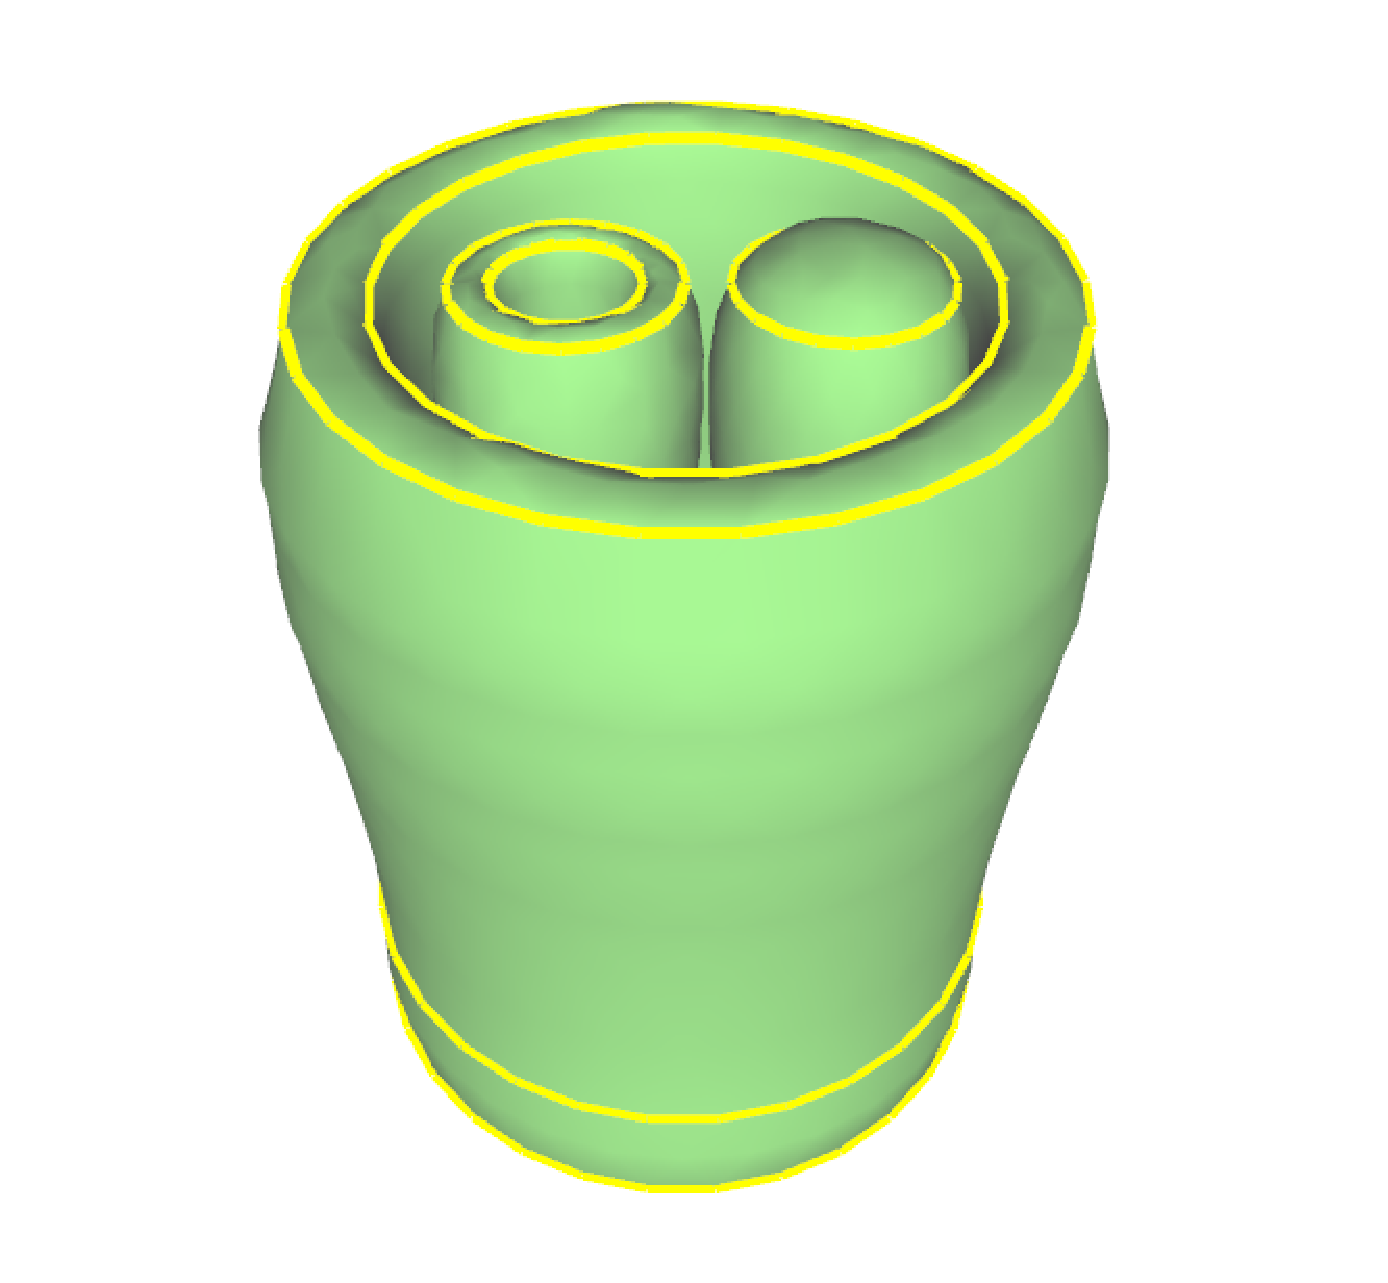
\includegraphics[scale=0.12]{figs/f3.rule2-2.eps}
    \end{minipage}}
  \caption{An example for rule~\ref{rule:2}. (a) The user sketched cross sections. Containing relationship exists among multiple cross sections on the blue plane; (b) The generated model.}
  \label{fig:rule2} %% label for entire figure
\end{figure}

Rule~\ref{rule:3} just does not allow self-intersection of one
curve or intersection between any two curves on the same plane since
it unlikely happens for the cross section contour of an object to
have intersection.

Rule~\ref{rule:4} can also be stated in another way that the
intersection points between the two curves and the intersection line
of the two planes must be be in the same positions. This rule
actually conforms to our common understanding of appearance of a 3D
object. It is difficult to imagine what the shape of the model will
be if the two sets $\{V_{S_1P_2}\}$ and $\{V_{S_2P_1}\}$ are not
same. However in practice, it is almost impossible for the users to
draw two exactly intersected curves manually. So after the curve
$S_1$ is drawn, we highlight the point set $\{V_{S_1P_2}\}$ to help
the users carefully draw the curve $S_2$ to make it pass through
$\{V_{S_1P_2}\}$ (see Figure~\ref{fig:csinters:a}). Then we perform
a curve deformation procedure, which is explained below, to
automatically sew the two curves up before constructing the surface.

For simplicity, let us assume there are two elements  in set
$\{V_{S_1P_2}\}$, which implies two curves $S_1$ and $S_2$ should
intersect at two points. So the goal here is to deform the two
curves, making them intersect at two points and meanwhile preserve
their original shape as much as possible.

First we calculate the intersection point set  $\{V_{S_1P_2}\}$
between $S_1$ and $P_2$, and $\{V_{S_2P_1}\}$ between $S_2$ and
$P_1$. Then we find two pairs of different closest points, in each
pair the two points are from $\{V_{S_1P_2}\}$ and $\{V_{S_2P_1}\}$
respectively. The midpoints $V_{m1}$ and $V_{m2}$ of these two pairs
are treated as the new positions of the handle points. Two handle
points on each curve can then be chosen as the points closest to
$V_{m1}$ and $V_{m2}$ respectively. Next a range of points near the
handles are to be moved with them and we need to compute their new
positions. So we could perform the Laplacian deformation algorithm
to the two curves to deform them. Since the two curves are both
planar, it can be further simplified into a 2D deformation problem
which can be precisely solved~\cite{ESA07}.

\begin{figure} [htbp]
  \centering
  \subfigure[]{
    \centering
    \label{fig:curvemerge:a} %% label for first subfigure
    \begin{minipage}[b]{0.25\textwidth}
      \centering
      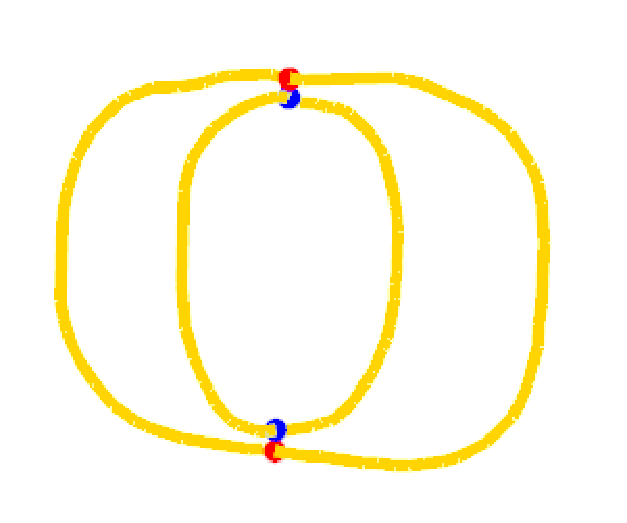
\includegraphics[scale=0.35]{figs/f3.CurveMerge1.eps}
    \end{minipage}}
  \subfigure[]{
    \centering
    \label{fig:curvemerge:b}
    \begin{minipage}[b]{0.25\textwidth}
      \centering
      
\includegraphics[scale=0.35]{figs/f3.CurveMerge2.eps}
    \end{minipage}}
  \subfigure[]{
    \centering
    \label{fig:curvemerge:c}
    \begin{minipage}[b]{0.25\textwidth}
      \centering
      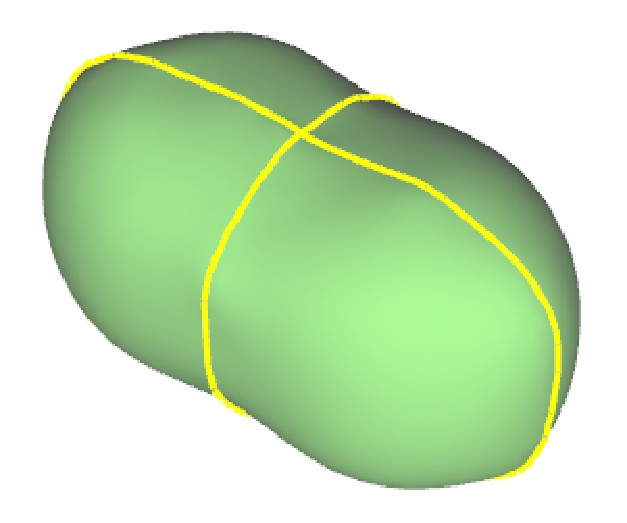
\includegraphics[scale=0.35]{figs/f3.CurveMerge3.eps}
    \end{minipage}}
  \caption{Curve sewing. (a) Two curves lie on two orthogonal planes. The colored points denote the intersection points between a curve and a plane that another curve lies on. (b) Deform the two curves so that they intersect at two points. (c) Generate a mesh that takes the two curves as contours.}
  \label{fig:curvemerge} %% label for entire figure
\end{figure}

It can be seen from Figure~\ref{fig:curvemerge} that  during the
deformation process, no extra discontinuity will be caused at the
intersection part of each curve and the deformed curves keep their
original shapes very well, thus preserving the original
characteristics of the user input strokes.

The above mentioned steps are for the simple two-contour  case. For
multiple contours, we just need to deal with them one by one to make
them accord with the rules we defined.

The curve sewing process can handle inconsistent cross sections
automatically, which meets the requirement on the user interface
design that the system should constructively suggest a solution to
help users to recover from errors~\cite{MN90}. By proposing these
rules and strategies, our sketching interface will become more
natural and intelligent to the user.

After all these processes, we are finally ready to construct  the
mesh model. The details on the progressive reconstruction algorithm
will be presented in Chapter~\ref{ch:orthsurf}.


\subsection{Reference plane calculation}
\label{ch3:sec:algo:refplane}

As mentioned in Section~\ref{ch3:sec:ui:sculpt:deform}, we provide
the users reference planes for drawing the deformed shape of the
handle curve in the deformation function. A key problem here is how
to generate the base plane which has a suitable position and
direction, as the projection plane could be easily calculated after
the base plane is confirmed.

Our basic idea is to let the base plane go through as many points of
the handle curve as possible. For this purpose, we compute the least
squares plane that fits the points. Assume the plane equation is

\begin{equation}
\label{eq:planefunc}
    Ax+By+Cz+D=0,
\end{equation}
where $A$, $B$, $C$ and $D$ are the unknown parameters to be determined,
and we let $A^2+B^2+C^2=1$, which means
$N = [\begin{array}{*{20}c} A & B & C \end{array}]$ is the unit normal
vector of the plane. Then our task is to find the plane that minimizes
the following objective function

\begin{eqnarray}
\label{eq:planeobjnoZ0}
    f(A,B,C,D) &=& \sum\limits_{i \in HC}
    {\frac {(Ax_i+By_i+Cz_i+D)^2}{A^2+B^2+C^2}},\nonumber\\
    &=& \sum\limits_{i \in HC} {(Ax_i+By_i+Cz_i+D)^2},
\end{eqnarray}
where $i \in HC$  means $p_i=(x_i,y_i,z_i)$ is a point on the handle curve.

%%%introduce the solving of this optimization problem
To solve this optimization problem, we used the method proposed
in~\cite{SWMB59}. First, we set the partial derivative of
$f(A,B,C,D)$ w.r.t. $D$ equal to zero and get:

\begin{eqnarray}
\label{eq:planeobjPartD}
    \sum\limits_{i \in HC} {(Ax_i+By_i+Cz_i+D)} = 0\nonumber\\
    D = -(Ax_c + By_c + Cz_c),
\end{eqnarray}
where $(x_c, y_c, z_c)$ represents the centroid of all the
input points on the handle curve. Then we substitute $D$ back
to Eq.~\ref{eq:planeobjnoZ0}, and the function to minimize can
be written as:

\begin{eqnarray}
\label{eq:planeobjnew}
    f(A,B,C) &=& \sum\limits_{i \in HC} {(A(x_i-x_c)+B(y_i-y_c)+C(z_i-z_c))^2}\nonumber\\
    &=& (NM^T)(MN^T)\nonumber\\
    &=& N (M^TM) N^T,
\end{eqnarray}
where $N = [\begin{array}{*{20}c} A & B & C \end{array}]$
is the unit normal vector of the plane we have mentioned
and $M$ is the matrix defined as:

\begin{equation*}
\begin{bmatrix}
x_1-x_c & y_1-y_c & z_1-z_c\\[-1em]
x_2-x_c & y_2-y_c & z_2-z_c\\[-1em]
\cdot & \cdot & \cdot\\[-1em]
\cdot & \cdot & \cdot\\[-1em]
\cdot & \cdot & \cdot\\[-1em]
x_n-x_c & y_n-y_c & z_n-z_c
\end{bmatrix},
\end{equation*}
assuming there are $n$ points on the handle curve. Next, $f(A,B,C)$
can be minimized by computing the singular value decomposition
of $M=USV^T$ and letting $P$ equal to the column of $V$ 
that corresponds to the smallest singular value of $M$.
To this end, the parameters of the optimal plane in
Eq.~\ref{eq:planefunc} can be obtained. It can be seen that
the calculated plane will interpolate the centroid of the
input points and its normal vector is the singular vector
of $M$ corresponding to its smallest singular value.

%%%


The above method just gives a suggestive orientation of the base
plane. If the user is not satisfied, he/she can rotate the plane by
a proper angle. The axis of the rotation is the line connecting the
projection of the first handle point onto the initial computed plane
to that of the last point. The calculation of the reference plane
for extrusion process is the same as this.

After the reference planes are constructed, the user can sketch the
new shape and position of the handle curve. If the user intends to
draw a non-planar curve by sketching the shadow of the base plane
curve on the projection plane, we use the algorithm proposed
in~\cite{CMZHB99} to combine the two planar curves to generate a
spatial one.

Once the ROI vertices, the handle curve and its new shape are
confirmed, we complete the deformation by employing a flexible mesh
deformation algorithm, which will be presented in
Chapter~\ref{ch:flexdeformation}.


%-------------------------------------------------------------------------
\section{Results and discussions}
\label{ch3:sec:result}

\begin{figure*} [htbp]
  \centering
  \subfigure[Mushroom]{
    \centering
    \label{fig:mushroom} %% label for first subfigure
    \begin{minipage}[b]{\textwidth}
      \centering
      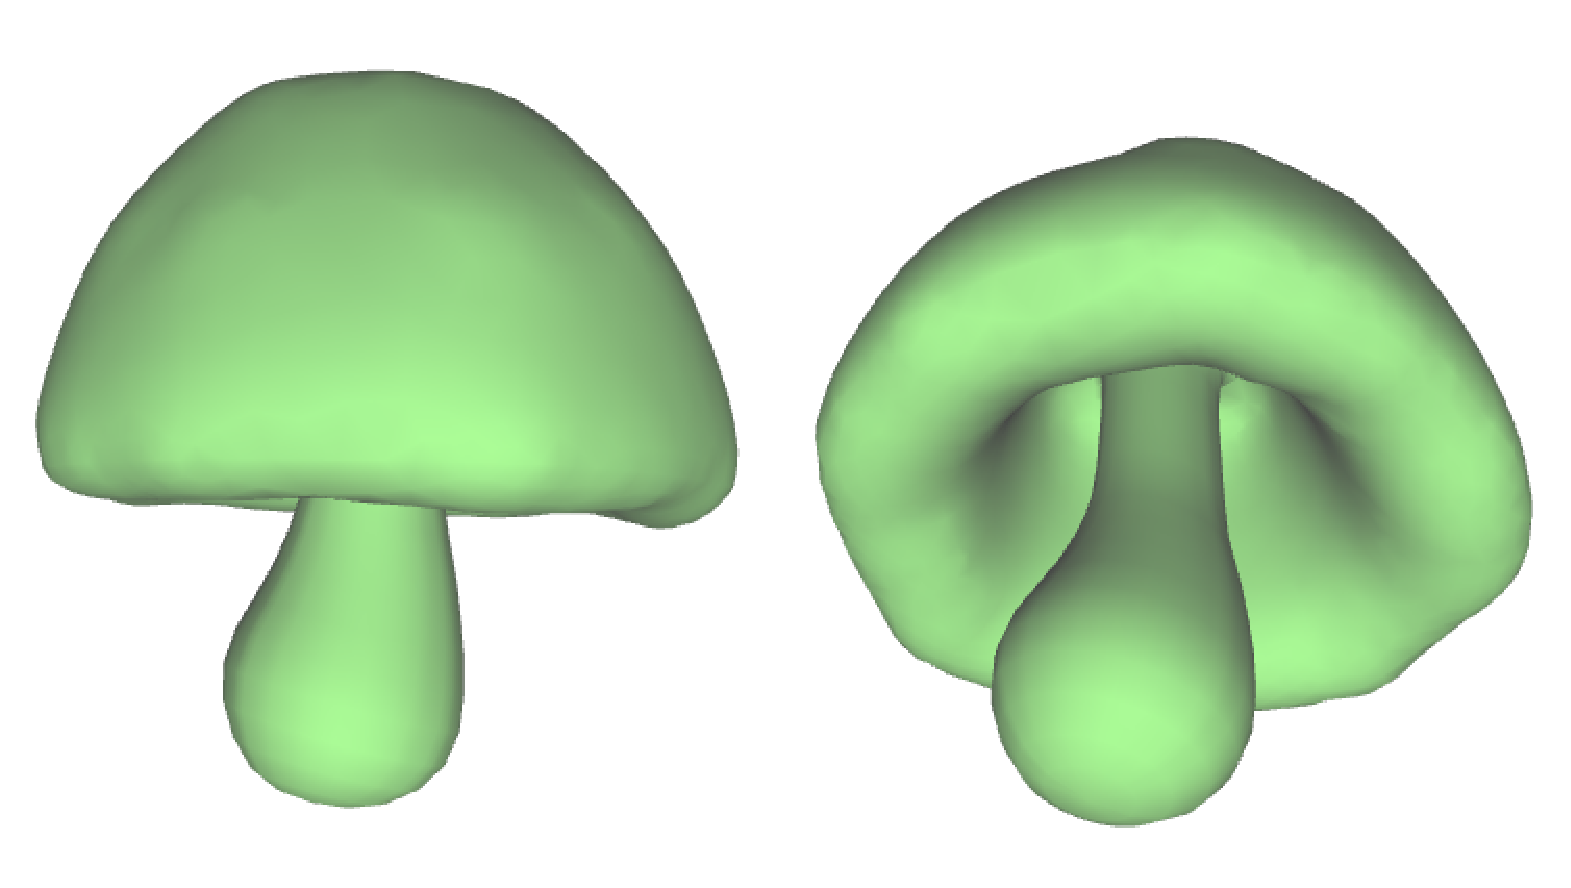
\includegraphics[scale=0.1]{figs/f3.mushroom.eps}%0.09
    \end{minipage}}
  \subfigure[Handicraft]{
    \centering
    \label{fig:6hole} %% label for first subfigure
    \begin{minipage}[b]{\textwidth}
      \centering
      \includegraphics[scale=0.1]{figs/f3.6hole.eps}
    \end{minipage}}
  \subfigure[Car]{
    \centering
    \label{fig:car} %% label for first subfigure
    \begin{minipage}[b]{\textwidth}
      \centering
      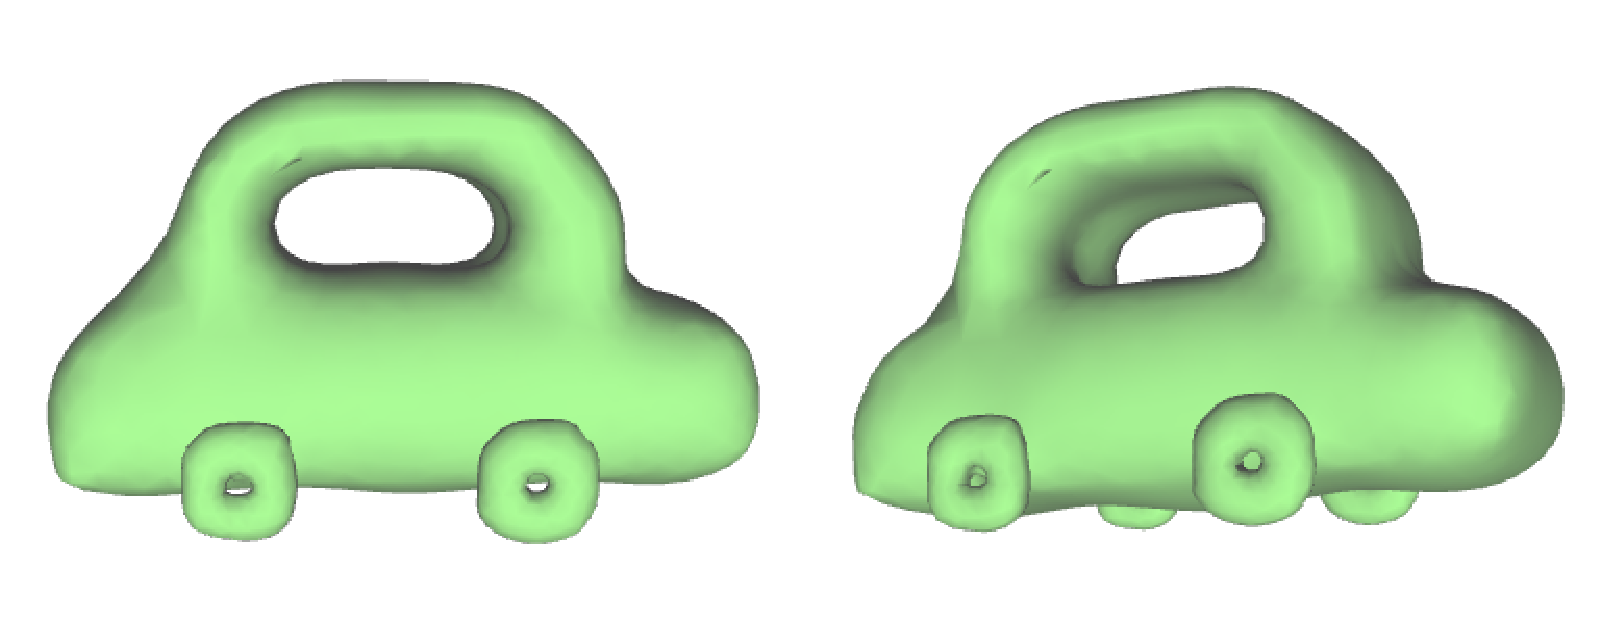
\includegraphics[scale=0.1]{figs/f3.car.eps}
    \end{minipage}}
  \subfigure[Censer]{
    \centering
    \label{fig:censer} %% label for first subfigure
    \begin{minipage}[b]{\textwidth}
      \centering
      \includegraphics[scale=0.1]{figs/f3.censer.eps}
    \end{minipage}}
  \subfigure[Bicycle]{
    \centering
    \label{fig:bike} %% label for first subfigure
    \begin{minipage}[b]{\textwidth}
      \centering
      \includegraphics[scale=0.1]{figs/f3.bike.eps}
    \end{minipage}}
  \subfigure[Sculpture]{
    \centering
    \label{fig:sculpture} %% label for first subfigure
    \begin{minipage}[b]{\textwidth}
      \centering
      \includegraphics[scale=0.1]{figs/f3.sculpture.eps}
    \end{minipage}}
  \caption{The sketching of some models using our system.}
  \label{fig:models:sketch} %% label for entire figure
\end{figure*}

\begin{figure*} [htbp]
  \subfigure[Cup]{
    \centering
    \label{fig:cup} %% label for first subfigure
    \begin{minipage}[b]{\textwidth}
      \centering
      \includegraphics[scale=0.12]{figs/f3.cup.eps}
    \end{minipage}}
  \subfigure[Rabbit]{
    \centering
    \label{fig:rabbit} %% label for first subfigure
    \begin{minipage}[b]{\textwidth}
      \centering
      \includegraphics[scale=0.12]{figs/f3.rabbit.eps}
    \end{minipage}}
  \subfigure[Chair]{
    \centering
    \label{fig:chair} %% label for first subfigure
    \begin{minipage}[b]{\textwidth}
      \centering
      \includegraphics[scale=0.12]{figs/f3.chair.eps}
    \end{minipage}}
  \caption{The sketching and sculpting of some models using our system.}
  \label{fig:models:combine} %% label for entire figure
\end{figure*}

%basic information
Our current implementation of this sketch-based modeling system was
written  in C++ on the Windows platform. We tested our system on an
machine with Dual Core Intel Xeon 2.27GHz CPU and 2G RAM. Our
experiments show that both the surface reconstruction and other
sculpting functions run in interactive rates. This indeed meets the
user's requirement on a sketch-based modeling system.

%computation complexity and cost
It is observed that even if multiple cross section curves are
sketched initially, the constructed mesh is not quite dense, and
the number of vertices will be no more a few thousands after
iterative editing operations. This enables us to consider more about
the modeling effect and quality of the mesh other than the running
time. Meanwhile, the modeling algorithms we developed also ensure
that computation will be completed in real time, which can be
introduced in the next chapters.

%For the surface reconstruction in our sketching tool, the shape built from each cross section is just simple cylinders, so the CSG computation is relatively simple and little numerical issues are involved. It is observed that even if multiple cross section curves are sketched initially, the constructed mesh is not quite dense, and the number of vertices will be no more a few thousands after iterative editing operations. This enables us to consider more about the modeling effect and quality of the mesh other than the running time.

%user study
We have conducted an informal user study to test our system.  We
trained the novice users for approximately 20 minutes and let them
create models with freeform shapes. We found that most users tend to
use the sketching tool to iteratively sketch and construct the 3D
models in most of the time and just take the sculpting tools to do
some detail modifications, although there are a few who prefer to
build a model by sculpting it from a rough shape (see
Figure~\ref{fig:chair}). This is consistent with the introduction
in~\cite{CIW08} that the sketching technique is more familiar to
public than sculpting which requires tedious manual work. Some
results produced with either the sketching tool or the combination
of the two tools are shown in Figure~\ref{fig:models:sketch} and
Figure~\ref{fig:models:combine}. All of these models are produced in
less than 30 minutes.

We learned from the feedback that with help of the reference planes,
the users can get a direct \lq\lq{touch}\rq\rq of the 3D space and
they only need to focus on the sketching of the curves for defining
the shape of the 3D model. The reference shape together with the
existing sketches let them get a clear mind of the 3D model in each
design stage and also give hints for the next sketches. Some issues
exist in other systems such as difficulties on confirming the
position and orientation of the 3D curves corresponding to the 2D
sketches, the imagination of the sketched 3D shape and so on can be
avoided. Although the users do not adapt to the stroke rules quite
well initially, they get used to it gradually with the help of
various hints in our system during the studying process and find it
quite helpful for eliminating perception ambiguities eventually.




%%-------------------------------------------------------------------------
%\section{Conclusions}
%\label{ch3:sec:concl}
%
%We have described a novel sketching interface for creating and editing 3D models. The main contributions are:
%
%\begin{itemize}
%   \item We propose a progressive modeling approach to enhance the creation function in sketch-based modeling, by allowing the user to create a 3D model through iterative sketches, taking both the existing sketches and the shape in each design stage as references. The user can thus get fully aware of the 3D shape which changes naturally with each new sketch and unexpected result can be avoided. Supporting surface reconstruction algorithm for this approach is developed to produce natural shape changes and models with single connected components.
%   \item We propose the strategy of using auxiliary planes as references for creation, deformation and other editing operations in the sketching interface. Reference planes help make the sketch-based modeling process intuitive and easy to use.
%   \item We propose stroke rules for regularizing and interpreting the user input sketches. These rules consider both the semantic meaning of the sketched strokes and human psychology.
%\end{itemize}
%
%In future, the surface reconstruction algorithm for the progressive modeling can be further accelerated using parallel computing or other techniques, since the computation within each zone is totally independent. In addition, we will explore the use of more types of geometry objects as references to assist sketch-based interface and modeling.


\chapter{Progressive Surface Reconstruction from Orthogonal Cross Sections}\label{ch:orthsurf}
This chapter presents the algorithm on progressive surface
reconstruction from orthogonal cross sections, which effectively
supports the sketching function in our sketch-based modeling system.

%=================section==================
\section{Introduction}
\label{ch4:sec:intro}
%==========================================

%introduction of surface reconstruction
Surface reconstruction from cross sections has already been a
widely-investigated problem for years. It has wide applications in
many areas of computer graphics and computer-aided design. The input
is usually a set of planar cross section curves which are extracted
from scanned 2D slices or sketched from scratch, and the output is a
smooth surface which interpolates the input curves.

%progressive surface reconstruction,input, output
In our sketch-based modeling system, the sketching function
requires reconstruction where the input is a set of cross sections
$CS=\{cs_i~|~i=1,...,m\}$ which are progressively sketched by the
users and lie on a set of orthogonal planes $P=\{p_i~|~i=1,...,n\}$
in 3D space $\mathbb{R}^3$. Each plane $p_i$ can be defined by
$x=d_i$, $y=d_i$ or $z=d_i$ ($d_i\in \mathbb{R}$). The cross
sections are represented as polylines. In the progressive modeling
process, the output in each step is expected to be a closed
2-manifold triangular mesh $M$ interpolating the sketched cross
sections $CS^\prime=\{cs_i~|~i=1,...,m^\prime, m^\prime\leq m\}$.
Each edge of $M$ is incident to two faces and the faces incident to
a vertex forms a closed fan.

As introduced in Section~\ref{ch2:sec:surfreconst}, most previous
works mainly focused on the reconstruction from parallel cross
sections, while recently Liu et al.~\cite{LBDLJ08} proposed a method
to reconstruct surfaces from more complicated non-parallel cross
sections. The method provides a more general solution to the surface
reconstruction problem and is useful in applications which only
require a final reconstruction result given all the input cross
sections. However, it cannot meet the some requirements in our
progressive sketching interface. Providing the cross sections are
valid under the stroke rules proposed in
Section~\ref{ch3:sec:algo:rule}, these requirements include:

%specific requirements on the algorithm
\begin{enumerate}
    \item The update of the model shape during the progressive modeling process should be gradual regardless of the input orders of the sketched curves, and unexpected shape change should be avoided.
    \label{req:1}
    \item The reconstructed model is expected to have only one connected component, when the user iteratively adds new sketches that are closely related to the shape in the current design stage.
    \label{req:2}
    \item The shape of the final model should be insensitive to the user's sketching order. In other words, given a same set of curves drawn with different orders, the reconstruction result should be unique.
    \label{req:3}
\end{enumerate}

The new surface reconstruction algorithm presented in the rest of
this chapter meets the above requirements.

%=================section==================
\section{Overview of the algorithm}
%\label{ch4:sec:algo}
%==========================================
%
%\subsection{Method overview}
\label{ch4:sec:algo:ov}

%2d illustration of surface reconstruction
\begin{figure*} [htbp]
  \centering
  \subfigure[]{
    \centering
    \label{fig:workflow2dortho:a}
    \begin{minipage}[b]{0.23\textwidth}
      \centering
      
\includegraphics[scale=0.6]{figs/f4.illu-workflow-2d1.eps}
    \end{minipage}}
  \subfigure[]{
    \centering
    \label{fig:workflow2dortho:b}
    \begin{minipage}[b]{0.23\textwidth}
      \centering
      
\includegraphics[scale=0.6]{figs/f4.illu-workflow-2d2.eps}
    \end{minipage}}
  \subfigure[]{
    \label{fig:workflow2dortho:c}
    \begin{minipage}[b]{0.23\textwidth}
      \centering
      
\includegraphics[scale=0.6]{figs/f4.illu-workflow-2d3.eps}
    \end{minipage}}
  \subfigure[]{
    \label{fig:workflow2dortho:d}
    \begin{minipage}[b]{0.23\textwidth}
      \centering
      
\includegraphics[scale=0.6]{figs/f4.illu-workflow-2d4.eps}
    \end{minipage}}
  \subfigure[]{
    \label{fig:workflow2dortho:e}
    \begin{minipage}[b]{0.23\textwidth}
      \centering
      
\includegraphics[scale=0.6]{figs/f4.illu-workflow-2d5.eps}
    \end{minipage}}
  \subfigure[]{
    \label{fig:workflow2dortho:f}
    \begin{minipage}[b]{0.23\textwidth}
      \centering
      
\includegraphics[scale=0.6]{figs/f4.illu-workflow-2d6.eps}
    \end{minipage}}
  \subfigure[]{
    \label{fig:workflow2dortho:g}
    \begin{minipage}[b]{0.23\textwidth}
      \centering
      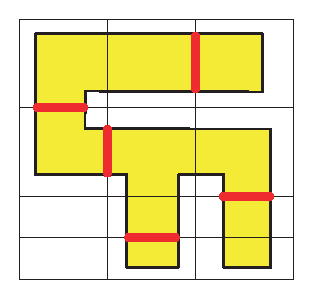
\includegraphics[scale=0.6]{figs/f4.illu-workflow-2d7.eps}
    \end{minipage}}
  \caption{2D illustration of our surface reconstruction algorithm.
  (a) Input segments (red, corresponding to the 3D cross sections) and partitioned zones;
  (b) The \textit{empty} zones (blue), \textit{end} zones (green) and \textit{body} zones (yellow);
  (c) Generating polygons (corresponding to the cylinders) in \textit{body} zones;
  (d) Generating polygons in the \textit{end} zones using the same way as the reconstruction in the \textit{body} zones. The reconstruction result contains multiple components;
  (e) Generating extended polygons for an \textit{end} zone;
  (f) Generating polygons for all \textit{end} zones;
  (g) The reconstruction result. }
  \label{fig:workflow2dortho}
\end{figure*}


%basic workflow
Similar to~\cite{LBDLJ08}, our algorithm also  follows the general
divide-and-conquer strategy. That is, we first place a large virtual
bounding box containing all the cross sections (we set its size to be 2 times
that of the bounding box of all points on the cross sections). This box will keep
fixed during the sketching process and all points on the input cross
sections will lie within it. Then we partition the box into zones
$ZN=\{zn_i~|~i=1,...,m\}$ using the planes that the cross sections
lie on. The shape of each zone $zn_i$ is thus a cuboid since we only
allows the translation of the orthogonal reference planes. Within
$zn_i$, the curves might be split into segments such that the segments
are entirely lie in the faces $F=\{f_{ij}~|~f_{ij}\in
zn_i,j=1,...,n\}$. Next we build a sub-surface which interpolates
the curve segments on the faces of each zone and stitch all the
pieces of sub-surfaces together to form a complete surface. Finally
we carry out constrained refinement and smoothing to the initial
mesh surface to improve its quality while maintaining its
interpolation on the input cross sections.

%limitation of TJ's method
Though the projection-based method in~\cite{LBDLJ08} can be used for
reconstruction, it will make the shape of the reconstructed surface
rely on that of the geometric agency (the MA plane) to a large
extent. In the progressive modeling process, each time a new cross
section is sketched on a new plane, the MA planes in the related
zones will be re-calculated, which probably leads to the shape
change of the surface components generated from all the cross
sections within these zones, and further the change of the
sub-surfaces. In that case, some surface parts generated from some
unrelated cross sections will be changed, resulting in unexpected
shape changes of the model surface. Especially in the iterative
sketching process, different input orders of a same set of sketched
curves will introduce different changes of the agencies, and the
shape changes will be unexpected under some input orders of the
curves. In other words, whether gradual shape changes can be
achieved or not depends on the sketching orders to some extent. Such
an example is shown in Figure~\ref{fig:csgma}. When new cross
sections are added following the order in Figure~\ref{fig:csgma:a},
unexpected shape change (breaking the originally connected
component) happened, which obviously goes against user's intention.

\begin{figure*} [htbp]
  \centering
  \subfigure[]{
    \centering
    \label{fig:csgma:a} %% label for first subfigure
    \begin{minipage}[b]{0.18\textwidth}
      \centering
      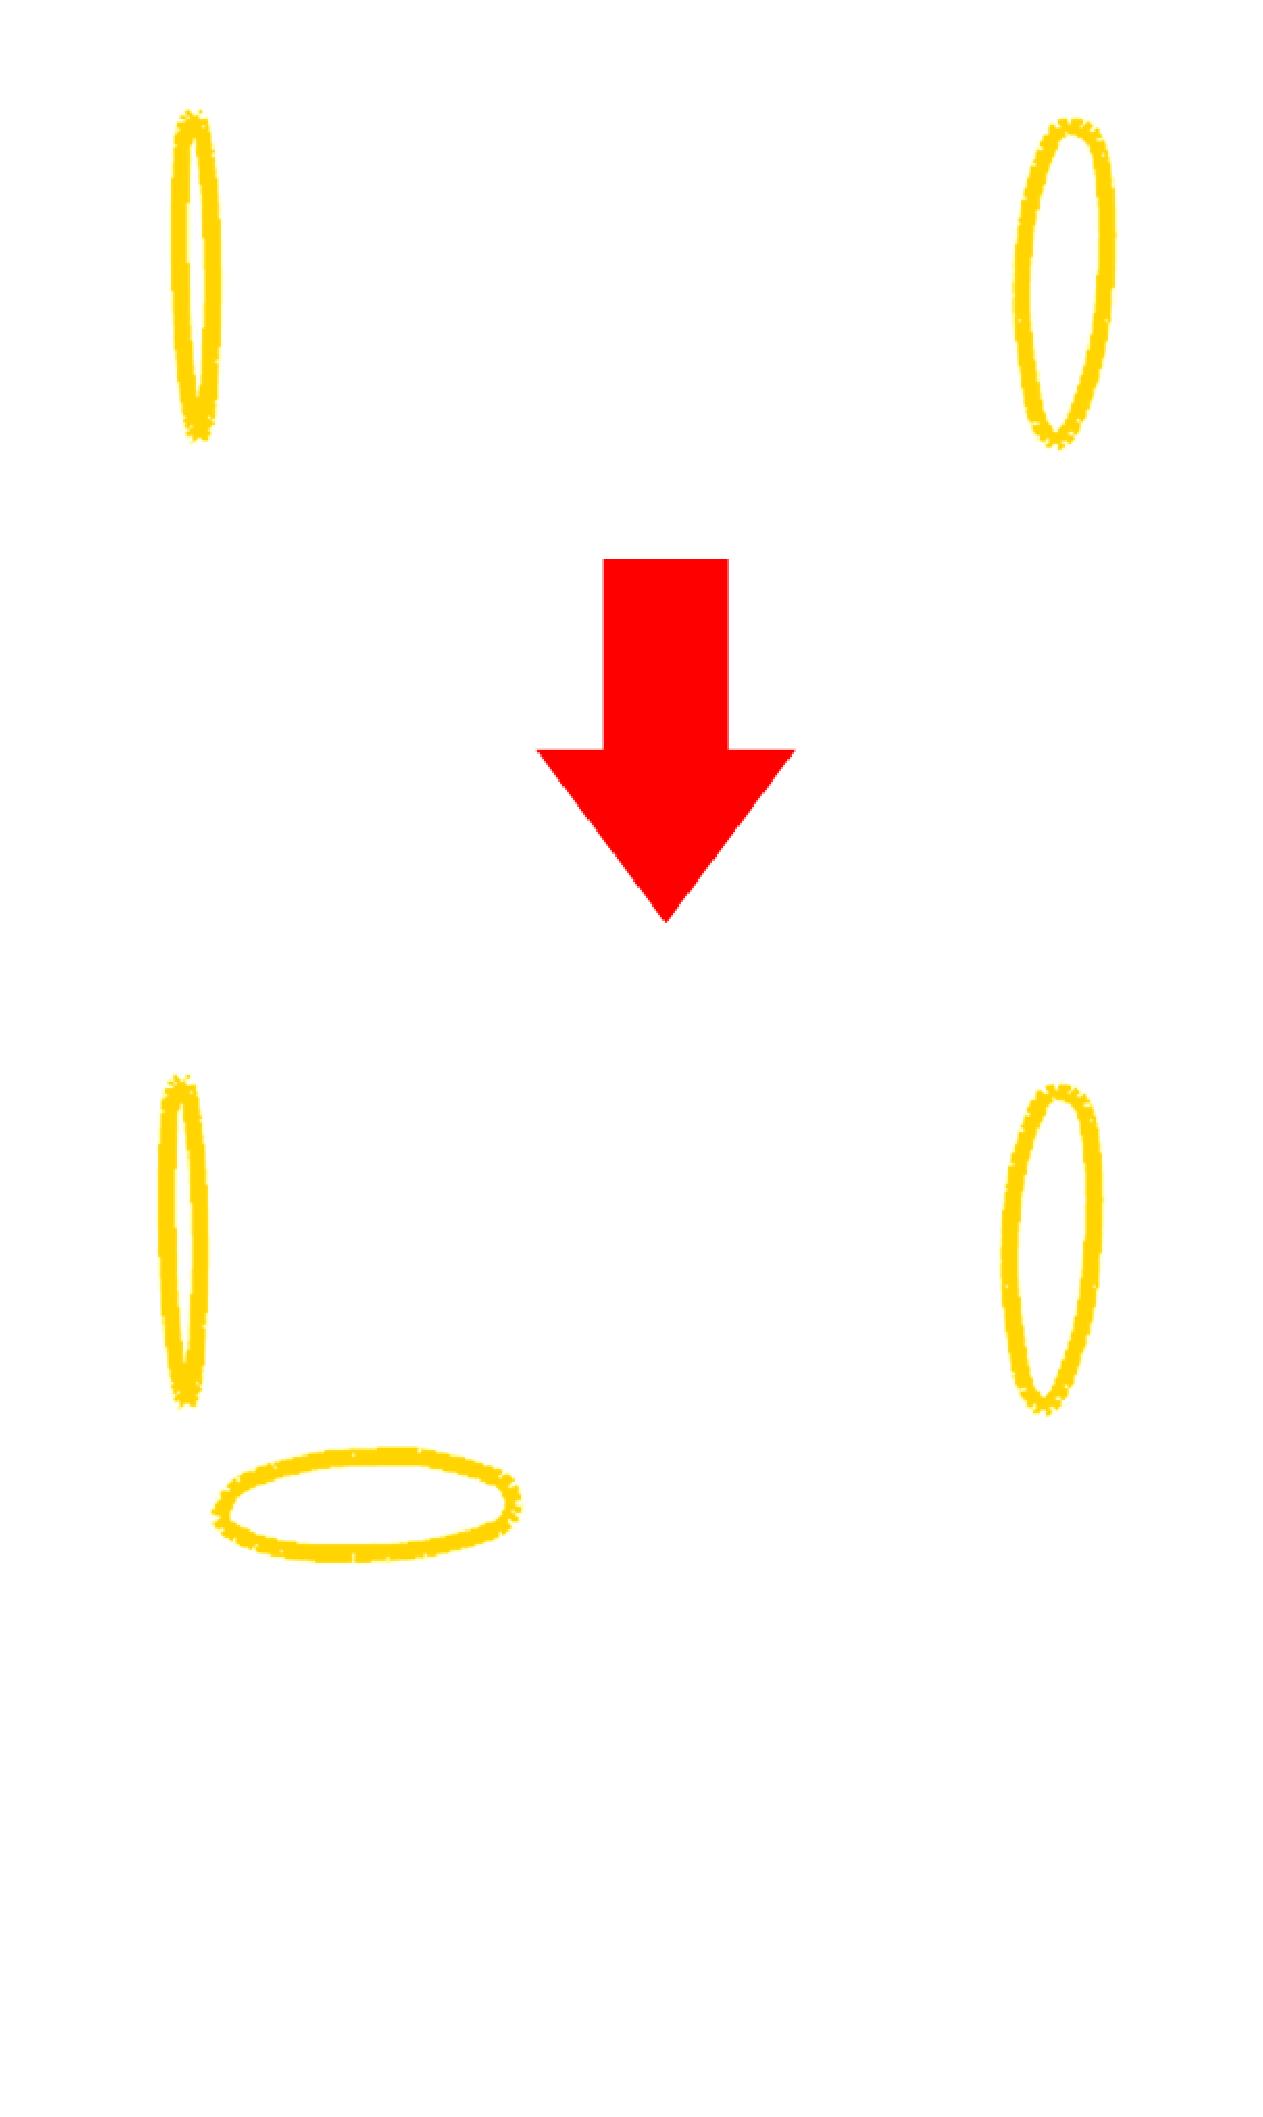
\includegraphics[scale=0.12]{figs/f3.surf-csgma-1.eps}
    \end{minipage}}
  \subfigure[]{
    \centering
    \label{fig:csgma:b}
    \begin{minipage}[b]{0.18\textwidth}
      \centering
      \includegraphics[scale=0.12]{figs/f3.surf-csgma-2.eps}
    \end{minipage}}
  \subfigure[]{
    \centering
    \label{fig:csgma:c}
    \begin{minipage}[b]{0.18\textwidth}
      \centering
      \includegraphics[scale=0.12]{figs/f3.surf-csgma-3.eps}
    \end{minipage}}
  \subfigure[]{
    \centering
    \label{fig:csgma:d}
    \begin{minipage}[b]{0.18\textwidth}
      \centering
      \includegraphics[scale=0.12]{figs/f3.surf-csgma-4.eps}
    \end{minipage}}
  \subfigure[]{
    \centering
    \label{fig:csgma:e}
    \begin{minipage}[b]{0.18\textwidth}
      \centering
      \includegraphics[scale=0.12]{figs/f3.surf-csgma-5.eps}
    \end{minipage}}
  \caption{An example of comparing our surface reconstruction algorithm  and that of~\cite{LBDLJ08}. (a) Two cross sections are sketched first and then one more is added; (b) The initial reconstruction results in~\cite{LBDLJ08}. The Medial Axis planes (blue) in a zone are shown; (c) The final reconstruction results in~\cite{LBDLJ08}; (d) The initial reconstruction results in our algorithm. The union of cylinders in each zone is shown; (e) The final reconstruction results in our algorithm.}
  \label{fig:csgma} %% label for entire figure
\end{figure*}

%motivation of the csg method
To get rid of the affection of the geometric agency and produce
gradual shape change during progressive modeling, we used a CSG
(Constructive Solid Geometry)-based method, instead of the
projection-based method to generate the sub-surface in each zone.
Our method is inspired by the work~\cite{RDI10}, which builds a 3D
model from 2D silhouettes sketched under orthogonal views by
generating cylinders from each silhouette and computing the union of
them. However, the inputs in our system are 3D cross sections with
different depths and complex mutual relationship, so the computation
will be more involved.

%csg method
Generally, in each zone $zn_i$, we build a cylinder from  each cross
section $cs_p$ and then compute the union of these cylinders.
Meanwhile, we extend some cylinders which may probably become
isolated surface components, to make them intersect with cylinders
in other zones and thus reduce the possibility of the existence of
multiple components of the final surface. The final surface is then
obtained by stitching all pieces of the sub-surfaces built in each
zone.

%zone types
Specifically, depending on the number of faces  having cross section
curves on, a zone is first classified into one of the following
three types:
\begin{itemize}
    \item A zone with no faces containing cross sections (denoted by an \textit{empty} zone),
    \item A zone with only one face containing cross sections (denoted by an \textit{end} zone),
    \item A zone with two or more faces containing cross sections (denoted by a \textit{body} zone).
\end{itemize}
Figure~\ref{fig:workflow2dortho} is a 2D illustration of such a
partition with three types of zones. The red segments on the lines
correspond to the cross sections on the zone faces.


In the next three sections, we will show how to create sub-surfaces in
the \textit{body} zones and \textit{end} zones and how to stitch
the sub-surfaces. For an \textit{empty} zone, it has no cross
sections and is thus ignored.




\section{Sub-surface reconstruction for a \textit{body} zone}
\label{ch4:sec:algo:body}

\begin{figure*} [htbp]
  \centering
  \subfigure[]{
    \centering
    \label{fig:cshape:a} %% label for first subfigure
    \begin{minipage}[b]{0.22\textwidth}
      \centering
      \includegraphics[scale=0.15]{figs/f3.surf-cshape-1.eps}
    \end{minipage}}
  \subfigure[]{
    \centering
    \label{fig:cshape:b}
    \begin{minipage}[b]{0.22\textwidth}
      \centering
      \includegraphics[scale=0.15]{figs/f3.surf-cshape-2.eps}
    \end{minipage}}
  \subfigure[]{
    \centering
    \label{fig:cshape:c}
    \begin{minipage}[b]{0.22\textwidth}
      \centering
      \includegraphics[scale=0.15]{figs/f3.surf-cshape-3.eps}
    \end{minipage}}
  \subfigure[]{
    \label{fig:cshape:d}
    \begin{minipage}[b]{0.22\textwidth}
      \centering
      \includegraphics[scale=0.15]{figs/f3.surf-cshape-4.eps}
    \end{minipage}}
  \subfigure[]{
    \label{fig:cshape:e}
    \begin{minipage}[b]{0.22\textwidth}
      \centering
      \includegraphics[scale=0.15]{figs/f3.surf-cshape-5.eps}
    \end{minipage}}
  \subfigure[]{
    \label{fig:cshape:f}
    \begin{minipage}[b]{0.22\textwidth}
      \centering
      \includegraphics[scale=0.15]{figs/f3.surf-cshape-6.eps}
    \end{minipage}}
  \subfigure[]{
    \label{fig:cshape:g}
    \begin{minipage}[b]{0.22\textwidth}
      \centering
      \includegraphics[scale=0.15]{figs/f3.surf-cshape-7.eps}
    \end{minipage}}
  \subfigure[]{
    \label{fig:cshape:h}
    \begin{minipage}[b]{0.22\textwidth}
      \centering
      \includegraphics[scale=0.15]{figs/f3.surf-cshape-8.eps}
    \end{minipage}}
  \caption{An example of surface reconstruction from non-intersected cross sections in the \textit{body} zones. (a) The input cross sections; (b) Partition result. The red planes are the bounding planes of each zone and the numbers represent the indices of the zones; (c)-(d) Cylinders generated from the two cross sections in Zone 1; (e) The union of cylinders in Zone 1; (f) The unions of cylinders in all zones; (g) The initial reconstruction result obtained by stitching surfaces in all zones; (h) The final reconstruction result after refinement and smoothing.}
  \label{fig:cshape} %% label for entire figure
\end{figure*}

%no intersection case
For a cross section $cs_p$ on face $f_{ij}$ which does  not
intersect with other cross sections in zone $zn_i$, we need to build
a cylinder $cl_p$ taking the 2D region enclosed by $cs_p$ as the
bottom $cl_p^b$. The initial top $cl_p^t$ of $cl_p$ is obtained by
translating $cl_p^b$ along the direction orthogonal to $f_{ij}$ and
pointing towards the inside of $zn_i$. Suppose the height of the
zone is $h_{zn}$ regarding $f_{ij}$ as the bottom face of the zone
(as we have introduced, each zone is a cuboid), the distance of the
translation $h_p$ (the height of $cl_p$) is then computed as:

\begin{equation}
\label{eq:clheight}
h_p = h_{zn}- \epsilon,
\end{equation}
where $\epsilon$ is a small positive number to make sure that the
center of $cl_p^t$ lie within $zn_i$. In this way, the cylinder
$cl_p$ will be totally contained in the zone $zn_i$ and interpolates
the input cross section $cs_p$. An example of the generation of the
cylinders in this case can be found in Figure~\ref{fig:cshape}.


\begin{figure*} [htbp]
  \centering
  \subfigure[]{
    \centering
    \label{fig:csinters:a}
    \begin{minipage}[b]{0.22\textwidth}
      \centering
      \includegraphics[scale=0.15]{figs/f3.surf-csinters-2.eps}
    \end{minipage}}
  \subfigure[]{
    \centering
    \label{fig:csinters:b}
    \begin{minipage}[b]{0.22\textwidth}
      \centering
      \includegraphics[scale=0.15]{figs/f3.surf-csinters-3.eps}
    \end{minipage}}
  \subfigure[]{
    \label{fig:csinters:c}
    \begin{minipage}[b]{0.22\textwidth}
      \centering
      \includegraphics[scale=0.15]{figs/f3.surf-csinters-4.eps}
    \end{minipage}}
  \subfigure[]{
    \label{fig:csinters:d}
    \begin{minipage}[b]{0.22\textwidth}
      \centering
      \includegraphics[scale=0.15]{figs/f3.surf-csinters-5.eps}
    \end{minipage}}
  \subfigure[]{
    \label{fig:csinters:e}
    \begin{minipage}[b]{0.22\textwidth}
      \centering
      \includegraphics[scale=0.15]{figs/f3.surf-csinters-6.eps}
    \end{minipage}}
  \subfigure[]{
    \label{fig:csinters:f}
    \begin{minipage}[b]{0.44\textwidth}
      \centering
      \includegraphics[scale=0.15]{figs/f3.surf-csinters-7.eps}
    \end{minipage}}
  \caption{An example of surface reconstruction from intersected cross sections in the \textit{body} zones. (a) The input cross sections. (b)-(c) Cylinders are generated from the two cross sections and perturbed; (d) The union of cylinders in the zone; (e) The initial reconstruction result; (f) The final reconstruction result after refinement and smoothing.}
  \label{fig:csinters} %% label for entire figure
\end{figure*}

%intersected case, need pertubation
When a cross section $cs_p$ on face $f_{ij}$  intersects with
another cross section $cs_q$ on the neighbor face $f_{ik}$ of
$f_{ij}$ in zone $zn_i$ (see Figure~\ref{fig:csinters:a}), computing
the cylinder $cl_p$ in the above method will make one face of $cl_p$
coincide with $f_{ik}$. As a result, the surface of the union of the
cylinders may probably not interpolate $cs_q$ on $f_{ik}$. In that
case, we first generate an initial cylinder $cl_p^{ini}$ from $cs_p$
in the above method. Then we perturb $cl_p^{ini}$ a little bit, by
translating a subset of points of $cl_p^t$ which lie on the neighbor
face $f_{ik}$ towards the center point of $cl_p^t$ a small distance,
such that there will not be any face of the result cylinder
$cl_p^{ptb}$ coincide with $f_{ik}$, and interpolation of the final
surface on $cs_q$ can thus be achieved. Strictly speaking,
$cl_p^{ptb}$ will not be a cylinder anymore, since the shapes of its
bottom and top are not the same after the perturbation. However,
this will not affect the union calculation which takes general
polyhedrons as input. Similarly, the cylinder $cl_q^{ptb}$ can be
generated from $cs_q$. The result surface after the union
calculation will lie in $zn_i$ and interpolate the input cross
sections (see Figure~\ref{fig:csinters:d}). This perturbation method
also works for the generation of a cylinder from a cross section
which intersects with other cross sections on multiple neighbor
faces.

\section{Sub-surface reconstruction for an \textit{end} zone}
\label{ch4:sec:algo:end}

%drawback of existing methods
Similar to the method in~\cite{LBDLJ08}, we use  the classical
partition method in Computational Geometry to divide the whole space
into zones and build sub-surfaces within each zone. However, this
strategy may cause the reconstructed model to have some isolated
components, because some faces which do not have cross sections on
will still take effect on forming the \textit{end} zones (the blue
faces in Figure~\ref{fig:partition:c}), and the cylinders generated
in these zones cannot connect to any other surface components except
those generated in the other incident zones of the faces containing
the cross sections. As a result, these cylinders may probably become
isolated surface components and the whole surface will thus be
composed of multiple components(see the 2D example in
Figure~\ref{fig:workflow2dortho:d} and 3D example in
Figures~\ref{fig:partition:f}).

In progressive modeling, when the user  gradually adds new sketches
that are closely related to the existing shape, the algorithm is
desired to produce a model with only one component. This is a
reasonable criterion that agrees with user's expectation. Therefore,
we adopt a strategy to extend the cylinders built in the
\textit{end} zones to other non-end zones (the \textit{body} and
\textit{empty} zones), to minimize their possibility of becoming
isolated surface components.

%detailed method
Specifically, for each cross  section $cs_p$ on face $f_{ij}$ in an
\textit{end} zone $zn_i$, we first build a cylinder $cl_p$ from
$cs_p$ using the same method as generating a cylinder from a
non-intersected cross section in a \textit{body} zone. Then we check
if the face $f_{ik}$ opposite to $f_{ij}$ in $zn_i$ belongs to the
bounding box or not. If yes, then the extension will be considered
as impossible and $cl_p$ will be treated as the surface component
generated from $cs_p$ in $zn_i$.

If $f_{ik}$ does not belong to the bounding box, the extension is
regarded as possible. In that case, $cl_p$ will be stretched into
the neighbor zone $zn_k$ of $zn_i$ that $f_{ik}$ incident to, along
the direction orthogonal to $f_{ij}$. The height of the $cl_p$ will
then taken as that of the zone $zn_i$ (regarding $f_{ij}$ as the
bottom), plus the computed height in zone $zn_k$ using
Eq.~\ref{eq:clheight} (regarding $f_{ik}$ as the bottom). If the
zone $zn_k$ is a body zone, or the face opposite to $f_{ik}$ in
$zn_k$ belongs to the bounding box, this extension process will
terminate and the extended $cl_p$ will be regarded as the surface
components generated from $cs_p$; Otherwise, $cl_p$ will be further
extended in the same way until these requirements are satisfied.

\begin{figure*} [htbp]
  \centering
  \subfigure[]{
    \centering
    \label{fig:partition:a} %% label for first subfigure
    \begin{minipage}[b]{0.3\textwidth}
      \centering
      \includegraphics[scale=0.14]{figs/f3.surf-end-1.eps}%0.12
    \end{minipage}}
  \subfigure[]{
    \centering
    \label{fig:partition:b}
    \begin{minipage}[b]{0.3\textwidth}
      \centering
      \includegraphics[scale=0.16]{figs/f3.surf-end-2.eps}%0.14
    \end{minipage}}
  \subfigure[]{
    \centering
    \label{fig:partition:c}
    \begin{minipage}[b]{0.3\textwidth}
      \centering
      \includegraphics[scale=0.16]{figs/f3.surf-end-3.eps}%0.14
    \end{minipage}}
  \subfigure[]{
    \centering
    \label{fig:partition:d}
    \begin{minipage}[b]{0.3\textwidth}
      \centering
      \includegraphics[scale=0.16]{figs/f3.surf-end-4.eps}%0.14
    \end{minipage}}
  \subfigure[]{
    \centering
    \label{fig:partition:e}
    \begin{minipage}[b]{0.3\textwidth}
      \centering
      \includegraphics[scale=0.14]{figs/f3.surf-end-5.eps}%0.12
    \end{minipage}}
  \subfigure[]{
    \centering
    \label{fig:partition:f}
    \begin{minipage}[b]{0.3\textwidth}
      \centering
      \includegraphics[scale=0.14]{figs/f3.surf-end-6.eps}%0.12
    \end{minipage}}
  \caption{An example of surface reconstruction in the \textit{end} and \textit{body} zones. (a) Input cross sections; (b) The partition result; (c) The extended cylinders for the \textit{end} zones.  The blue faces are those which may cause isolated surface components; (d) The unions of cylinders in all zones; (e) Final surface reconstruction result in our approach; (f) Reconstruction result using the algorithm in~\cite{LBDLJ08}.}
  \label{fig:partition} %% label for entire figure
\end{figure*}

As shown in Figure~\ref{fig:partition}, by extending the cylinders
built in the \textit{end} zones to make them intersect with other
cylinders, isolated surface components can be connected to form a
single component. While for the projection-based method
in~\cite{LBDLJ08}, this extension is not easy to implement, and the
result surface will contain multiple isolated components.

%isolated part cannot be totally eliminated
It should be pointed out that this cylinder extension  strategy
cannot guarantee the final surface to always have a single
component. Such cases may happen when cylinders within the same zone
cannot intersect whatever their heights are (such as the two
cylinders in Zone 6 in Figure~\ref{fig:cshape:f}). Although this
problem can be fixed by changing the shape of the cylinders to force
them connect regardless of the positions of the sketched cross
sections, we do not launch such a process since it may produce
irregular and undesired local shapes. Meanwhile, since the user
usually tends to add a new sketch that is closely related to the
current shape, if an isolated part is to be generated during the
sketching process, a hint will be given to the user to indicate that
possibility caused by the newly added sketch.


\section{Global surface reconstruction} \label{ch4:sec:algo:global}

%After all the cylinders in each zone are built, we use the algorithm
%proposed in~\cite{LTH86} to compute the union of them. The algorithm
%computes the unions of the input polyhedrons by getting those of the
%faces and glue them together, and it is robust and quick enough for
%our application since the shape of the polyhedrons are regular. The
%global surface of the initial mesh $M_{init}$ can then be calculated
%as:

%%%%%%%%%%%%%%%%%%%%%%%%%%%%%%%%%%%%%%%%%%%%%%%%%%%%%%%%%%%%%%%%%%
%%%%%%%%%added in thesis only
After all the cylinders in each zone are built, we use the
CarveCSG library~\cite{CarveCSG} which implements the algorithm proposed
in~\cite{LTH86} to compute the union of these polyhedrons one by one.

Given two polyhedrons $P_a$ and $P_b$, each triangle $Tr^a_i$ on $P_a$ will be
visited first. If $Tr^a_i$ intersects with a triangle $Tr^b_j$ on $P_b$, then
both $Tr^a_i$ and $Tr^b_j$ will be bisected by the plane of each other's.
This way, $P_a$ and $P_b$ will become new polyhedrons $P^\prime_a$ and
$P^\prime_b$ which are composed of bisected triangles. Next, the triangles on
$P^\prime_a$ which are inside the volume of $P^\prime_b$, as well as
those on $P^\prime_b$ inside the volume of $P^\prime_a$ will be removed.
Finally, the left triangles from $P^\prime_a$ and $P^\prime_b$ will
be merged and the union result can be obtained.

This method is robust and quick enough for our application since the shape
of the polyhedrons are regular. The global surface of the initial mesh
$M_{init}$ can then be calculated as:
%%%%%%%%%added in thesis only
%%%%%%%%%%%%%%%%%%%%%%%%%%%%%%%%%%%%%%%%%%%%%%%%%%%%%%%%%%%%%%%%%%


\begin{equation}
\label{eq:surfreconstortho}
    M_{init}=\sum\limits_{i=1}^m {(Cl_{i1} \bigcup Cl_{i2} \bigcup {...} \bigcup Cl_{in})}
\end{equation}
where $Cl_{ij}$ refers to the $j$th cylinder built in  the $i$th
zone, assuming there are totally $m$ zones and $n$ cylinders in each
zone.

\subsection{Mesh improvement}
\label{ch4:sec:algo:global:improve}

Since the shape of the initially reconstructed surface $M_{init}$ is usually unnatural and jaggy, we then improve it through iterative refinement and smoothing.

%%%%%%%%%%%%%%%%%%%%%%%%%%%%%%%%%%%%%%%%%%%%%%%%%%%%%%%%%%%%%%%%%%
%%%%%%%%%modified in the revised thesis
For the mesh refinement, we used the algorithm proposed in~\cite{LP03} to produce a result similar to the Delaunay-like triangulation through iterative triangle splitting and edge swapping. 

First, we compute the length attribute $\sigma_i$ for each vertex $v^0_i$ on the input cross sections as the average length of all the edges adjacent to $v^0_i$. The attribute for
each neighbor vertex $v^1_i$ of $v^0_i$ which is not on the input cross sections will
be computed as the average of $\sigma_i$ of all $v^0_i$s which are neighbors of $v^1_i$.
The length attributes for all other vertices will be computed ring by ring in 
this propagation way.

Then, for each triangle $(v_i, v_j, v_k)$, we compute its centroid $v_c$ and the 
length attribute $\sigma_c$ for $v_c$ as 
$\sigma_c= (\sigma_i + \sigma_j + \sigma_k)/3$. For each vertex $\{v_m | m=i, j, k\}$ 
of this triangle, if $\alpha ||v_m-v_c||> \sigma_c$ and $\alpha ||v_m-v_c||> \sigma_m$
(we set $\alpha=\sqrt{2}$ as suggested in~\cite{LP03}),
we then replace the triangle $(v_i, v_j, v_k)$ with triangles $(v_i, v_j, v_c)$,
$(v_j, v_k, v_c)$ and $(v_k, v_i, v_c)$, and relax the edges $(v_i, v_j)$, $(v_j, v_k)$
and $(v_k, v_i)$.

Here relaxing an edge $(v_i, v_j)$ means for the two triangles $(v_i, v_j, v_k)$ and
$(v_i, v_j, v_n)$ adjacent to $(v_i, v_j)$, we check if $v_k$ and $v_n$ lie inside
the triangles $(v_i, v_j, v_n)$ and $(v_i, v_j, v_k)$ respectively. If yes, we implement 
the edge swapping to let the two triangles become $(v_i, v_k, v_n)$ and $(v_j, v_k, v_n)$.
To ensure the interpolation on the input curves, this edge swapping is restricted to 
the edges which do not belong to the input cross sections.

If there are new triangles created in the above step, we relax all the edges and
repeat this step; otherwise, the refinement process is complete.



%%%%%%%%%modified in the revised thesis
%%%%%%%%%%%%%%%%%%%%%%%%%%%%%%%%%%%%%%%%%%%%%%%%%%%%%%%%%%%%%%%%%%

For the mesh smoothing, we adopted the algorithm in~\cite{YB02} to produce meshes with smooth shapes. The initial surface is evolved by first moving each vertex along its normal direction to minimize the local curvature differences. Then to improve the computational stability, the triangle sizes are made as equal as possible by moving the vertices along the tangential direction. These two movements are implemented iteratively on the vertices that do not lie on the input cross section curves.

In our implementation, we alternatively refine and smooth the initial mesh for 10 iterations. The result surface will have satisfactory quality and its interpolation on the input cross sections is maintained.


%=================section==================
\section{Results and discussions}
\label{ch4:sec:disc}
%==========================================

%advantage of our method
Examples produced by our sketch-based modeling  system using the
CSG-based progressive surface reconstruction algorithm can be found
in Figure~\ref{fig:models:sketch}.

By making use of the cylinders which reflect the shape and
positions of the sketched cross sections in the reconstruction
process, our approach can get rid of the MA plane, whose change is
more complicated during progressive sketching and will lead to
unexpected shape change of the surface parts generated from
unrelated cross sections. As a result, the change of the model shape
will be natural under any sketching orders, which meets
Requirement~\ref{req:1} for our sketching system. An example showing
this advantage of our CSG-based method over the projection-based
method in~\cite{LBDLJ08} can be found in Figure~\ref{fig:csgma}.

%why order insensitive
In the reconstruction process, the extension of the cylinders in
the isolated zones, as well as the union calculation of the
cylinders in all zones are carried out independently. So for a same
set of sketches, the final reconstruction result will be unique and
insensitive to its input orders.

%other advantages of the CSG-based method, local calculation
There are also some other advantages of the  CSG-based method which
have been utilized in our progressive modeling interface. For
example, since the calculations within each zone are independent,
each time the user adds, modifies or deletes a cross section, only
the sub-surfaces in the affected zones need to be recalculated and
updated, while those in other zones can be retained. In this way,
the calculation can be implemented locally and accelerated.

%partial cross section: stroke rules+subzone+previewed shape and computed cross sections
The independence of calculation in each zone also makes it possible
to allow the sketching of only a part of the cross section instead
of a complete one, as long as the stroke rules are satisfied within
the zone. Since the user sketches are more or less arbitrary, we
also perform automatic curve sewing similar to that mentioned in
Section~\ref{ch3:sec:algo:rule} or give user related hints, to make
sure the stroke rules are followed.

%progressive surface reconstrucion: not only in sbim, but also applications input progressively and require real-time reconstruction result, such as ultra-sound...
Although the CSG-based progressive surface reconstruction  algorithm
is designed for the sketching operation in our system, it can also
be used in other applications such as the CT or ultrasound scan, in
which the input cross sections are obtained from gradually scanned
slices. By making use of our algorithm, the reconstructed 3D model
can be built progressively and its shape can be updated in a natural
manner to provide the user desired real-time feedback.


\chapter{Triangular Mesh Deformation via Edge-Based Graph}\label{ch:flexdeformation}
%This chapter considers one of the supporting algorithms for sketch-based modeling system introduced in Chapter~\ref{ch:planeSBIM} -- the surface-based mesh deformation algorithm. Surface deformation for triangular meshes has become a popular research topic in computer graphics and geometric modeling. Most of the existing mesh deformation methods establish their formulations in the primal vertex-based domain and are expected to produce globally smooth and consistent deformation results while preserving geometry details as much as possible. In this chapter, we present a new surface-based mesh deformation method that performs the computation via an edge-based graph to increase the sampling rate for more accurate shape computation and better deformation results. The user is given the flexibility of adjusting the deformation effect between local shape preservation and global smoothness. Moreover, to simulate the deformation behaviors of regions with different materials, we introduce a stiffness property into the deformation model and present an easy and intuitive way for the user to set the material property. Experimental results demonstrate that our algorithm can produce satisfactory results and make the deformation more flexible.
This chapter presents an edge-based flexible mesh deformation
algorithm, which effectively supports the deformation function in
our sketch-based modeling system.

%=================section==================
\section{Introduction}
\label{ch5:sec:intro}
%==========================================
Mesh deformation is an effective and convenient  method for mesh
editing in geometric modeling and computer animation, and it is also
an important sculpting function in sketch-based modeling systems. It
allows the user to manipulate one part or the entire surface while
preserving some geometric characteristics of the initial surface. As
 introduced in Section~\ref{ch2:sec:deformation}, various
algorithms on mesh deformation have been developed due to its
importance and popularity in a wide rage of applications in
industrial and artistic designs. Though having their respective
advantages, those algorithms also have drawbacks due to the
following considerations in mesh deformation.

First, a triangular mesh is a piecewise linear  surface and it is
often considered as an approximation of some unknown smooth surface.
The approximation effect is related to the number of vertices of the
mesh. In general, the larger the number of vertices the mesh
contains, the better is the approximation. When a deformation is
performed on a surface, the calculation will be conducted on the
vertices. The number of vertices determines the sampling rate in
approximating a continuous model and thus a denser mesh usually
results in more accurate deformation. However, given a deformation
region, the number of vertices is fixed and it is not trivial to
have more points be involved in the deformation calculation.

Second, in the deformation process the local  shape feature is often
required to be well preserved and the deformed shape should be
natural and smooth to satisfy aesthetics or other requirements. A
natural problem then arises: what is a good balance between the
rigidity and fairness? The answer is subjective. A satisfactory
editing result depends on the algorithm adopted, the specific models
and the desired effect as well.

Third, an object in real world may be  composed of different
materials, which may exhibit different behaviors when the object is
deformed. For example, with different stiffness properties of the
materials, different deformation effects between rigidity and
smoothness will appear under the deformation. Most of the existing
deformation methods are purely geometrically-based and they ignore
the material properties of the object.

To solve these problems and make the  deformation more flexible, we
propose a flexible mesh deformation algorithm which performs the
computation through an edge-based graph. Instead of formulating the
deformation on the primal domain, we build an edge-based graph and
carry out the deformation computations on the graph, which involves
more nodes and thus produces better deformation results. We then
propose a mixed energy model that combines the first order and the
second order discrete differential quantities to balance local shape
preservation and smoothness. The user can adjust the values of the
balance parameter to control the deformation results. Moreover,
these introduced balance parameters are used to reflect the
stiffness property of the object material and thus make the
deformation algorithm material-aware. A simple sketching tool is
provided to specify the stiffness property. The novelty of the
chapter thus lies in the use of the edge-based graph for the
deformation formulation and the use of balance parameters for
controlling the stiffness and producing various reasonable
deformation results in a mesh deformation task.



%==========================================
\section{Edge-based graph} \label{ch5:sec:alg:edgegraph}
Let
$M=(V,E)$ be a triangular mesh with $n$ vertices. $V=\{v_i|v_i\in
R^3,i=1,...,n\}$ denotes the set of vertices and
$E=\{e_{ij}=(v_i,v_j)|v_i,v_j\in V,i\neq j\}$ represents the set of
edges. Correspondingly, we define $\tilde{M}=(\tilde{V},\tilde{E})$
as the corresponding edge-based graph for $M$, where
$\tilde{V}=\{\tilde{v_i}|\tilde{v_i}\in R^3,i=1,...,n_e\}$ and
$\tilde{E}=\{\tilde{e_{ij}}=(\tilde{v_i},\tilde{v_j})|\tilde{v_i},\tilde{v_j}\in
\tilde{V},i\neq j\}$ are the sets of nodes and edges of the
edge-based graph respectively. Specifically, a node $\tilde{v_i}$ is
defined as the midpoint of the edge $e_{ij}$  in the primal domain:
$\tilde{v_i}=(v_i+v_j)/2$. $n_e$ represents the number of nodes in
the edge-based graph, which equals the number of edges on the primal
mesh $M$. Each node $\tilde{v_i}$ corresponding to primal edge
$e_{ij}$ is connected to four neighboring nodes corresponding to the
four primal edges that share the vertices of $e_{ij}$. In this way,
the valence of each node in the edge-based graph is always four. The
conversion from the primal vertex positions $V$ to the edge-based
graph vertex positions $\tilde{V}$ can be accomplished by an
$n_e\times n$ sparse matrix $D$. Each row of $D$ has two non-zero
elements that are 1/2. Figure~\ref{fig:edgebasedgraph} shows an
edge-based graph constructed from a primal mesh.

\begin{figure} [htbp]
    \centering
  \includegraphics[scale=0.6]{figs/f5.2.edge-based-graph.eps}
  \caption{An illustration of an edge-based graph. The black lines represent the primal mesh and the green lines form the edge-based graph.}
  \label{fig:edgebasedgraph} %% label for entire figure
\end{figure}



%==========================================
\section{Flexible mesh deformation} \label{ch5:sec:alg:flexdefo}
In  mesh deformation, the user first  specifies the \textit{handle}
vertices and their new positions, as well as the \textit{static}
vertices that will remain unchanged, and then the algorithm
determines the deformation of the \textit{region-of-interest (ROI)}
vertices. Many previous deformation algorithms aim to preserve
either the first or the second order discrete differential
quantities of the mesh surface and thus can produce only one kind of
deformation result, which may be either too rigid or smooth.

We present  a method that considers both of the two differential
quantities and balances between the rigidity and smoothness of the
deformation in a flexible manner. Our basic idea is to deform the
vertices in the ROI such that a mixed energy functional is minimized
and this minimization problem is formulated on an edge-based graph.
The mixed energy functional includes the change of the first order
and second order differential quantities that reflect stretching and
bending. Based on Euler-Poincare formula, the number of edges on a
triangular mesh is approximately three times that of vertices. Thus
the energy functional formulated on the edge-based graph better
approximates the continuous version of the energy functional of the
smooth surface than that on the primal domain. Thus the formulation
on the edge-based graph tends to render better deformation results,
especially when rigid or smooth deformation effects are required.
See Figure~\ref{fig:deformbaby} for an example.

\begin{figure} [htbp]
  \centering
  \subfigure[]{
    \centering
    \label{fig:deformbaby:a} %% label for first subfigure
    \begin{minipage}[b]{0.3\textwidth}
      \centering
      \includegraphics[scale=0.35]{figs/f5.1.baby-pc-3.eps}
    \end{minipage}}
   \\
  \subfigure[]{
    \centering
    \label{fig:deformbaby:b}
    \begin{minipage}[b]{0.3\textwidth}
      \centering
      \includegraphics[scale=0.35]{figs/f5.1.ver0-iso-3.eps}
    \end{minipage}}
  \subfigure[]{
    \centering
    \label{fig:deformbaby:c}
    \begin{minipage}[b]{0.3\textwidth}
      \centering
      \includegraphics[scale=0.35]{figs/f5.1.ver05-iso-3.eps}
    \end{minipage}}
  \subfigure[]{
    \centering
    \label{fig:deformbaby:d}
    \begin{minipage}[b]{0.3\textwidth}
      \centering
      \includegraphics[scale=0.35]{figs/f5.1.ver10-iso-3.eps}
    \end{minipage}}
  \\
  \subfigure[]{
    \centering
    \label{fig:deformbaby:e} %% label for first subfigure
    \begin{minipage}[b]{0.3\textwidth}
      \centering
      \includegraphics[scale=0.35]{figs/f5.1.edge0-iso-3.eps}
    \end{minipage}}
  \subfigure[]{
    \centering
    \label{fig:deformbaby:f}
    \begin{minipage}[b]{0.3\textwidth}
      \centering
      \includegraphics[scale=0.35]{figs/f5.1.edge05-iso-3.eps}
    \end{minipage}}
  \subfigure[]{
    \centering
    \label{fig:deformbaby:g}
    \begin{minipage}[b]{0.3\textwidth}
      \centering
      \includegraphics[scale=0.35]{figs/f5.1.edge10-iso-3.eps}
    \end{minipage}}
  \caption{Flexible deformation of the \textit{Baby} model. (a) The initial model. (b)-(d) Results of the flexible deformation algorithm performed on the primal domain, with the global balance parameters valued 0, 0.5 and 1.0 respectively. (e)-(g) Results of the flexible deformation algorithm performed via the edge-based graph, with the global balance parameters valued 0, 0.5 and 1.0 respectively.}
  \label{fig:deformbaby} %% label for entire figure
\end{figure}






%==========================================
\subsection{First and second order discrete differential
quantities} First of all we need to find proper  representations for
the first and second order discrete differential quantities of the
mesh surface.

For a smooth surface, the  first order differential properties are
usually represented by length, area, etc. However, these will make
the system nonlinear. So for triangular meshes we choose to use edge
vectors at each node, which we called the 1-form, to represent the
first order differential structures of the mesh surface. The 1-form
contains the information of edge lengths and can help to make the
final system a linear one.

Specifically, for a  node $\tilde{v_i}$, the 1-form can be
represented by the edge vectors $\tilde{e_{ij}}$ which start from
the one-ring neighborhood $\tilde{v_j},\tilde{e_{ij}}\in \tilde{E}$
and point to $\tilde{v_i}$, as shown in
Figure~\ref{fig:edgebasedoneform}. It can totally decide the shape
of the local area around a node. That is to say, as long as the edge
vectors connecting $\tilde{v_i}$ and its neighbors are fixed, the
shape of the local area around $\tilde{v_i}$ is fixed.

The second order differential properties of  a smooth surface are
usually represented by curvatures, which also make the system a
nonlinear one~\cite{ESP08}. The Laplacian vector provides a proper
choice for representing the second order differential properties of
the mesh surface, since its magnitude approximates the mean
curvature at each vertex and the final system formed is a linear
one. So we extend the traditional definition of Laplacian vector
from the primal mesh to the edge-based graph and use it to represent
the second order discrete differential quantity of the mesh surface,
as shown in Figure~\ref{fig:edgebasedlap}.

\begin{figure} [htbp]
  \subfigure[]{
    \centering
    \label{fig:edgebasedoneform}
    \begin{minipage}[b]{0.45\textwidth}
      \centering
      \includegraphics[scale=0.8]{figs/f5.3.Rigid.eps}
    \end{minipage}}
  \subfigure[]{
    \centering
    \label{fig:edgebasedlap}
    \begin{minipage}[b]{0.45\textwidth}
      \centering
      \includegraphics[scale=0.8]{figs/f5.3.Laplacian.eps}
    \end{minipage}}
  \caption{(a) The 1-form. (b) The Laplacian vector.}
  \label{fig:edgebasedoneformlap} %% label for entire figure
\end{figure}

Mathematically, the Laplacian vector $\tilde{\delta_i}$ at $\tilde{v_i}$ is defined as:

\begin{equation}
\label{eq:edgelaplacian}
\tilde{\delta_i}=L(\tilde{v_i})=\sum\limits_{j\in N(i)}{\tilde{\omega_{ij}} (\tilde{v_i}-\tilde{v_j})},
\end{equation}
where $N(i)=\{j|\tilde{e_{ij}}\in \tilde{E}\}$ is the  index set of
adjacent nodes in the neighboring ring of $\tilde{v_i}$ and
$\tilde{\omega_{ij}}$ is the weight of the edge $\tilde{e_{ij}}$.
Here we use the cotangent weight scheme~\cite{MDSB02} to compute
$\tilde{\omega_{ij}}$. In fact, $L(\cdot)$ can be regarded as the
discretized Laplace-Beltrami operator with cotangent coefficients on
triangular meshes~\cite{BS08}.

It should be noted that the Laplacian  vector $\tilde{\delta_i}$ in
the edge-based graph can also be regarded as a measurement of the
dihedral angle $\alpha_i$ of two adjacent triangles in the primal
mesh, which also represents the second order differential property
of the mesh surface. The magnitude of $\tilde{\delta_i}$ is
inversely proportional to the size of $\alpha_i$, as can be seen in
Figure~\ref{fig:edgebaseddihedral}.

\begin{figure} [htbp]
  \subfigure[]{
    \centering
    \label{fig:edgebaseddihedral1}
    \begin{minipage}[b]{0.45\textwidth}
      \centering
      \includegraphics[scale=0.8]{figs/f5.4.dihedral1.eps}
    \end{minipage}}
  \subfigure[]{
    \centering
    \label{fig:edgebaseddihedral2}
    \begin{minipage}[b]{0.45\textwidth}
      \centering
      \includegraphics[scale=0.8]{figs/f5.4.dihedral2.eps}
    \end{minipage}}
  \caption{The Laplacian vector $\tilde{\delta_i}$ in the edge-based graph and the dihedral angle $\alpha_i$ between adjacent faces in the primal domain. (a) The shorter $\tilde{\delta_i}$ is, the larger $\alpha_i$ will be. (b) The longer $\tilde{\delta_i}$ is, the smaller $\alpha_i$ will be. }
  \label{fig:edgebaseddihedral} %% label for entire figure
\end{figure}

These two representations  of discrete differential quantities
encode the relative position of each node w.r.t. its neighboring
nodes and represent the local geometry properties of the mesh
surface. Next we will introduce how to combine them to get a
satisfactory deformation result flexibly.

%==========================================
\subsection{Energy function for flexible deformation} The approach
for solving  the deformation problem of the surface-based method is
to designate the positional constraints for the handle and static
vertices and solve for the positions of the ROI vertices by fitting
the local geometry properties of the deformed mesh to those of the
initial mesh. The properties we want to preserve include both the
first and second order discrete differential properties, which are
represented by the 1-form and Laplacian vectors.

Since the 1-form at each node $\tilde{v_i}$ can  totally decide the
shape of a local neighborhood area, it is considered as defining the
local shape of the mesh surface in a unique manner. Mathematically,
to preserve the 1-form of the initial mesh, the energy we try to
minimize for each node $\tilde{v_i}$ is:

\begin{equation}
\label{eq:edgerigidenergy}
E(\tilde{v_i}^\prime)=\sum\limits_{j\in N(i)}{\tilde{\omega_{ij}} ||\tilde{e_{ij}}^\prime -R_i \tilde{e_{ij}}||^2},
\end{equation}
where $\tilde{v_i}^\prime$ is the new  position of $\tilde{v_i}$,
$\tilde{e_{ij}}=\tilde{v_i}-\tilde{v_j}$ and
$\tilde{e_{ij}}^\prime=\tilde{v_i}^\prime-\tilde{v_j}^\prime$ are
the undeformed and deformed edge vectors between $\tilde{v_i}$ and
$\tilde{v_i}$ respectively. $\tilde{\omega_{ij}}$ is the same weight
as that in Eq.~\ref{eq:edgelaplacian}. $R_i$ represents the rotation
matrix associated to $\tilde{v_i}$. The optimal rotation matrix
$R_i$ can be calculated given the old and new values of the edge
vectors. Detailed deduction can be found in~\cite{SA07}.

The rigid transformation of the 1-form during  deformation strives
to do a \textit{hard} transform to the mesh. We say \textit{hard} as
the edge vectors of each node can completely determine the shape of
its neighborhood area. As long as each vector keeps fixed, the shape
of this area will not change at all.

To preserve each Laplacian vector of the mesh  surface during
deformation, we try to minimize its change up to an affine
transformation $T_i$. Since shearing and anisotropic scale will lead
to distortions of the local features~\cite{FAT07}, we assume $T_i$
be composed of rotation and isotropic scale, i.e. $T_i=s_iR_i$.
$s_i$ and $R_i$ represent the scale coefficient and rotation matrix
separately. The energy to minimize is:

\begin{equation}
\label{eq:edgelapenergy}
E(\tilde{v_i}^\prime)=||\sum\limits_{j\in N(i)}{\tilde{\omega_{ij}}(\tilde{v_i}^\prime - \tilde{v_j}^\prime)} -T_i\sum\limits_{j\in N(i)}{\tilde{\omega_{ij}}(\tilde{v_i} - \tilde{v_j})}||^2.
\end{equation}

The deformation of preserving the Laplacian vectors  is a relatively
\textit{soft} deformation, comparing to the \textit{hard} one, since the
Laplacian vector cannot exactly represent the shape of the local
area around each node. The word \textit{soft} has another meaning
that the deformed shape tends to be smooth, since the change of the
second order differential quantity is minimized to prevent the sharp
change of the mesh shape within a local area.

Up to now, we have obtained two linear methods for  mesh deformation
by preserving the 1-form and Laplacian vectors respectively. The
unknowns in the two systems are both the set of deformed node
positions. However, neither of the two methods can satisfy our
requirement of obtaining various deformation effects between
rigidity and smoothness. In the first method, while the
representation of the local shape is quite accurate, sometimes the
deformation will be too rigid that smoothness cannot be obtained.
Besides, a definite rigid transformation means that scale is not
considered, and thus some local features cannot be preserved under
this kind of transformation. In the second method, since the
Laplacian vector cannot exactly represent the shape of a local
region, local shape preservation may not be achieved. However, the
deformation calculated using this method is relatively smooth.
Moreover, scale transformation is considered in the computation to
make the result more natural and help to preserve the local features
under stretching or shrinking.

To make use of the advantages of these two methods and  give the
user flexibilities to choose the most desirable deformation effect
between rigidity and smoothness subject to a specific model, we
propose a new algorithm which combines the two methods using a
balance parameter $\lambda$. When $\lambda=1$, only the first order
discrete differential quantity of each node is preserved and the
deformation is the most rigid; when $\lambda=0$, only the second
order discrete differential quantities are preserved and a smooth
result is achieved. Multiple intermediate results can be obtained by
setting different $\lambda$ values between 0 and 1.

Considering the positional  constraints $\{\tilde{c_i}\},i\in
\{m,...,n\},m<n$, the overall energy we aim to minimize for a mesh
deformation task with $n$ nodes involved is:

\begin{eqnarray}
\label{eq:edgelocflexenergy}
E(V^\prime) &=& \sum\limits_{i=1}^n{\lambda_i(\sum\limits_{j\in N(i)}{\tilde{\omega_{ij}} ||\tilde{e_{ij}}^\prime -R_i \tilde{e_{ij}}||^2})}+\nonumber\\
& & \sum\limits_{i=1}^n{(1-\lambda_i)||\sum\limits_{j\in N(i)}{\tilde{\omega_{ij}}(\tilde{v_i}^\prime - \tilde{v_j}^\prime)} -T_i\sum\limits_{j\in N(i)}{\tilde{\omega_{ij}}(\tilde{v_i} - \tilde{v_j})}||^2}+\nonumber\\
& &\sum\limits_{i=m}^n{||\tilde{v_i}^\prime-\tilde{c_i}||^2},
\end{eqnarray}
in which the first and second  items of the right hand side are the
energies measured by the change of the 1-form and Laplacian vectors
and the third item is the positional constraints during deformation.
The balance parameter $\lambda_i (0\leq \lambda_i\leq 1)$ is used to
control the rigidity and smoothness of the deformation at node
$\tilde{v_i}$.

It is not difficult to see that the definitions  of 1-form and
Laplacian vectors and the flexible deformation algorithm can be
easily transferred to the primal domain, by replacing the variables
defined in the edge-based graph in Eq.~\ref{eq:edgelocflexenergy}
with those of the primal domain. This is useful for comparing the
deformation results calculated directly in the primal domain and via
the edge-based graph. Detailed comparisons can be found in
Section~\ref{ch5:sec:results}.


%==========================================
\subsection{Solving of the system} To solve this system, we use an
iterative method  which can be outlined as follows.

First we build an edge-based graph for the  deformation region of
the mesh and then compute the partial derivatives of the first and
second items in energy function~\ref{eq:edgelocflexenergy} w.r.t.
the unknown node positions $\tilde{V}^\prime$ and get two linear
systems $A_1\tilde{V}^\prime=b_1$ and $A_2\tilde{V}^\prime=b_2$. An
important observation is that if the coefficients $\lambda_i$ and
$1-\lambda_i$ are not considered, $A_1$ and $A_2$ happen to be the
same. So only one of them needs to be constructed in the beginning
and we just need to focus on the calculation of the right hand side
of the system in each iteration.

Then an initial deformation result is  estimated using the naive
Laplacian deformation~\cite{AM01} which does not consider rotation
and scale transformations of the Laplacian vectors. Based on the
estimated vertex positions, we can compute the rotation matrix $R_i$
and the transformation matrix $T_i$. Since the optimal $R_i$ can be
uniquely calculated through singular value
decomposition~\cite{SA07}, we make use of it to compute the optimal
scale coefficient $s_i$, such that $T_i=s_iR_i$ can be obtained.
This way, computations of $R_i$ and $T_i$ are associated and the
overall calculation process is accelerated. The right hand side of
the system is then updated by multiplying the calculated $R_i$ and
$T_i$ and the system can be solved.

Next some iterations are performed for  recomputing $R_i$ and $T_i$,
updating the right hand side of the system and solving it. This
process continues until convergence.

As all the above computations are  performed in the edge-based
graph, we need to reconstruct the primal mesh by using the
conversion matrix $D$ introduced in
Section~\ref{ch5:sec:alg:edgegraph} as well as the positional
constraints for primal handle and static vertices. However, since
the position of each node in the edge-based graph can be represented
as the linear combination of two primal vertex positions, an easier
way to solve the system is to integrate $D$ into
Eq.~\ref{eq:edgelocflexenergy} and directly take the primal vertex
positions as unknowns.



%==========================================
\section{Specification of the balance parameters}

In the preceding section we assume that the  balance parameters have
been predefined and treat them as constants during the calculation.
Now we  provide two methods to specify the balance parameters: a
global method and a local method.

In the global method, we let the  balance parameter $\lambda_i$ for
each node $\tilde{v_i}$ equal to the same value $\lambda$, such that
energy function~\ref{eq:edgelocflexenergy} turns to:

\begin{eqnarray}
\label{eq:edgeglbflexenergy}
E(V^\prime) &=& \lambda\sum\limits_{i=1}^n{(\sum\limits_{j\in N(i)}{\tilde{\omega_{ij}} ||\tilde{e_{ij}}^\prime -R_i \tilde{e_{ij}}||^2})}+\nonumber\\
& & (1-\lambda)\sum\limits_{i=1}^n{||\sum\limits_{j\in N(i)}{\tilde{\omega_{ij}}(\tilde{v_i}^\prime - \tilde{v_j}^\prime)} -T_i\sum\limits_{j\in N(i)}{\tilde{\omega_{ij}}(\tilde{v_i} - \tilde{v_j})}||^2}+\nonumber\\
& &\sum\limits_{i=m}^n{||\tilde{v_i}^\prime-\tilde{c_i}||^2}.
\end{eqnarray}

This global method provides a  proper choice when the user wants to
make the entire editing region of a mesh deform in a consistent
manner. The rigidity and smoothness of the deformation can be well
balanced through setting a proper $\lambda$ value between 0 and 1.
The user can select a proper $\lambda$ value to produce a
satisfactory result, according to the specific model and the
deformation effect he needs. Generally speaking, larger $\lambda$
values make the deformation more rigid and smaller $\lambda$ values
make it more fair. It can be seen that previous methods which
preserve either the first or the second order differential
properties of the mesh surface is just a special case of
Eq.~\ref{eq:edgeglbflexenergy}.

Examples of the global method  can be seen in
Figures~\ref{fig:deformdino} to~\ref{fig:deformJCglb}.

Although the global method  provides an efficient way of calculating
a natural and consistent deformation result for the entire editing
region, it ignores the individual property of each local area on the
mesh surface and sometimes is not flexible. So we also provide a
local method for the specification of the balance parameters.

Since objects in the real world  are often composed of non-uniformly
distributed materials, their deformation behaviors vary from
rigidity to smoothness across the surface, depending on the
stiffness of the materials on each local region. However, current
mesh deformation algorithms either ignore the underlying materials
of the mesh surface or suffer from various problems. The physics or
skeleton based algorithms provide feasible approaches to solve this
problem. Nevertheless, they are either slow in computation or
limited to a subset of models~\cite{PJS05}.

Since the balance parameter can be used to  control the rigidity and
smoothness of the deformation, we can use it to define the stiffness
property of the material on each local area of the mesh surface,
such that the regions with different materials will have
distinguished behaviors in a same deformation task. In this case,
$\lambda_i$ for each $\tilde{v_i}$ in Eq.~\ref{eq:edgelocflexenergy}
should be defined separately according to the material property of
$\tilde{v_i}$. The larger $\lambda_i$ is, the stiffer the material
will be and the deformation at $\tilde{v_i}$ should be relatively
rigid; otherwise, the material will be softer and the deformation
should be smooth.

\begin{figure} [htbp]
  \centering
  \subfigure[]{
    \centering
    \label{fig:deformdino:a} %% label for first subfigure
    \begin{minipage}[b]{0.32\textwidth}
      \centering
      \includegraphics[scale=0.29]{figs/f5.5.original_pc-2.eps}
    \end{minipage}}
   \\
  \subfigure[]{
    \centering
    \label{fig:deformdino:b}
    \begin{minipage}[b]{0.32\textwidth}
      \centering
      \includegraphics[scale=0.29]{figs/f5.5.ver0-3.eps}
    \end{minipage}}
  \subfigure[]{
    \centering
    \label{fig:deformdino:c}
    \begin{minipage}[b]{0.32\textwidth}
      \centering
      \includegraphics[scale=0.29]{figs/f5.5.ver05-3.eps}
    \end{minipage}}
  \subfigure[]{
    \centering
    \label{fig:deformdino:d}
    \begin{minipage}[b]{0.32\textwidth}
      \centering
      \includegraphics[scale=0.29]{figs/f5.5.ver10-3.eps}
    \end{minipage}}
  \\
  \subfigure[]{
    \centering
    \label{fig:deformdino:e} %% label for first subfigure
    \begin{minipage}[b]{0.32\textwidth}
      \centering
      \includegraphics[scale=0.29]{figs/f5.5.edge0-3.eps}
    \end{minipage}}
  \subfigure[]{
    \centering
    \label{fig:deformdino:f}
    \begin{minipage}[b]{0.32\textwidth}
      \centering
      \includegraphics[scale=0.29]{figs/f5.5.edge05-3.eps}
    \end{minipage}}
  \subfigure[]{
    \centering
    \label{fig:deformdino:g}
    \begin{minipage}[b]{0.32\textwidth}
      \centering
      \includegraphics[scale=0.29]{figs/f5.5.edge10-3.eps}
    \end{minipage}}
  \caption{Flexible deformation of the \textit{Dinosaur} model. (a) The initial model. (b)-(d) Results of flexible deformation algorithm performed on the primal domain, with the global balance parameters valued 0, 0.5 and 1.0 respectively. (e)-(g) Results of flexible deformation algorithm performed via the edge-based graph, with the global balance parameters valued 0, 0.5 and 1.0 respectively. }
  \label{fig:deformdino} %% label for entire figure
\end{figure}

Here we provide sketching  tools, which are intuitive and flexible
for interactive designs, for the user to designate materials on
different parts of the mesh surface. The user can first set a scalar
value which represents the stiffness property of the material and
then use lasso or painting brush tools to specify the material for
the selected part. Since the entire user operations are performed on
the surface of the primal mesh while the calculations are implicitly
implemented on the edge-based graph, after the materials of the
primal vertices are specified, we calculate the material for each
node $\tilde{v_i}$ of the edge-based graph by averaging those of the
two end vertices of the primal edge $e_{ij}$ that $\tilde{v_i}$ lies
on.


\begin{figure} [htbp]
  \centering
  \subfigure[]{
    \centering
    \label{fig:deformbuf:a} %% label for first subfigure
    \begin{minipage}[b]{0.32\textwidth}
      \centering
      \includegraphics[scale=0.32]{figs/f5.6.original-pc-1.eps}
    \end{minipage}}
  \subfigure[]{
    \centering
    \label{fig:deformbuf:b}
    \begin{minipage}[b]{0.32\textwidth}
      \centering
      \includegraphics[scale=0.32]{figs/f5.6.0flexible-3.eps}
    \end{minipage}}
  \subfigure[]{
    \centering
    \label{fig:deformbuf:c}
    \begin{minipage}[b]{0.32\textwidth}
      \centering
      \includegraphics[scale=0.32]{figs/f5.6.2flexible-3.eps}
    \end{minipage}}
  \\
  \subfigure[]{
    \centering
    \label{fig:deformbuf:d}
    \begin{minipage}[b]{0.32\textwidth}
      \centering
      \includegraphics[scale=0.32]{figs/f5.6.5flexible-3.eps}
    \end{minipage}}
  \subfigure[]{
    \centering
    \label{fig:deformbuf:e} %% label for first subfigure
    \begin{minipage}[b]{0.32\textwidth}
      \centering
      \includegraphics[scale=0.32]{figs/f5.6.8flexible-3.eps}
    \end{minipage}}
  \subfigure[]{
    \centering
    \label{fig:deformbuf:f}
    \begin{minipage}[b]{0.32\textwidth}
      \centering
      \includegraphics[scale=0.32]{figs/f5.6.10flexible-3.eps}
    \end{minipage}}
  \caption{Flexible deformation of the \textit{Buffle} model via the edge-based graph under different balance parameter values. (a) The initial model. (b)-(f) Deformation results with the global balance parameters valued 0, 0.2, 0.5, 0.8, 1.0 respectively. }
  \label{fig:deformbuf} %% label for entire figure
\end{figure}

\begin{figure} [htbp]
  \centering
  \subfigure[]{
    \centering
    \label{fig:deformJCglb:a} %% label for first subfigure
    \begin{minipage}[b]{0.32\textwidth}
      \centering
      \includegraphics[scale=0.25]{figs/f5.7.julius--Caesar-pc-1.eps}
    \end{minipage}}
  \subfigure[]{
    \centering
    \label{fig:deformJCglb:b}
    \begin{minipage}[b]{0.32\textwidth}
      \centering
      \includegraphics[scale=0.25]{figs/f5.7.0flexible-1.eps}
    \end{minipage}}
  \subfigure[]{
    \centering
    \label{fig:deformJCglb:c}
    \begin{minipage}[b]{0.32\textwidth}
      \centering
      \includegraphics[scale=0.25]{figs/f5.7.2flexible-1.eps}
    \end{minipage}}
  \\
  \subfigure[]{
    \centering
    \label{fig:deformJCglb:d}
    \begin{minipage}[b]{0.32\textwidth}
      \centering
      \includegraphics[scale=0.25]{figs/f5.7.5flexible-1.eps}
    \end{minipage}}
  \subfigure[]{
    \centering
    \label{fig:deformJCglb:e} %% label for first subfigure
    \begin{minipage}[b]{0.32\textwidth}
      \centering
      \includegraphics[scale=0.25]{figs/f5.7.8flexible-1.eps}
    \end{minipage}}
  \subfigure[]{
    \centering
    \label{fig:deformJCglb:f}
    \begin{minipage}[b]{0.32\textwidth}
      \centering
      \includegraphics[scale=0.25]{figs/f5.7.10flexible-1.eps}
    \end{minipage}}
  \caption{Flexible deformation of the \textit{Julius-Caesar} model via the edge-based graph under different balance parameter values. (a) The initial model. (b)-(f) Deformation results with the global balance parameters valued 0, 0.2, 0.5, 0.8, 1.0 respectively. }
  \label{fig:deformJCglb} %% label for entire figure
\end{figure}


Results of the local method can be seen in Figures~\ref{fig:deformplane} to~\ref{fig:deformpig}.

\begin{figure} [htbp]
  \centering
  \subfigure[]{
    \centering
    \label{fig:deformplane:a} %% label for first subfigure
    \begin{minipage}[b]{0.7\textwidth}
      \centering
      \includegraphics[scale=0.20]{figs/f5.8.planeMat2.eps}
    \end{minipage}}
  \\
  \subfigure[]{
    \centering
    \label{fig:deformplane:b}
    \begin{minipage}[b]{0.32\textwidth}
      \centering
      \includegraphics[scale=0.20]{figs/f5.8.ver0-iso-1.eps}
    \end{minipage}}
  \subfigure[]{
    \centering
    \label{fig:deformplane:c}
    \begin{minipage}[b]{0.32\textwidth}
      \centering
      \includegraphics[scale=0.20]{figs/f5.8.ver10-iso-1.eps}
    \end{minipage}}
  \subfigure[]{
    \centering
    \label{fig:deformplane:d}
    \begin{minipage}[b]{0.32\textwidth}
      \centering
      \includegraphics[scale=0.20]{figs/f5.8.verMat-iso-1.eps}
    \end{minipage}}
  \caption{Material-constrained deformation result of the \textit{plane} model. (a) The initial model and its specified materials. (b)-(c) Deformation results of uniformly distributed materials with global balance parameter valued 0 and 1 respectively. (d) Deformation result with the specified non-uniform materials.}
  \label{fig:deformplane} %% label for entire figure
\end{figure}

\begin{figure} [htbp]
  \centering
  \subfigure[]{
    \centering
    \label{fig:deformJCMat:a} %% label for first subfigure
    \begin{minipage}[b]{0.7\textwidth}
      \centering
      \includegraphics[scale=0.18]{figs/f5.9.JSMat2.eps}
    \end{minipage}}
  \\
  \subfigure[]{
    \centering
    \label{fig:deformJCMat:b}
    \begin{minipage}[b]{0.23\textwidth}
      \centering
      \includegraphics[scale=0.18]{figs/f5.9.ver0-iso-1.eps}
    \end{minipage}}
  \subfigure[]{
    \centering
    \label{fig:deformJCMat:c}
    \begin{minipage}[b]{0.23\textwidth}
      \centering
      \includegraphics[scale=0.18]{figs/f5.9.ver05-iso-1.eps}
    \end{minipage}}
  \subfigure[]{
    \centering
    \label{fig:deformJCMat:d}
    \begin{minipage}[b]{0.23\textwidth}
      \centering
      \includegraphics[scale=0.18]{figs/f5.9.ver10-iso-1.eps}
    \end{minipage}}
  \subfigure[]{
    \centering
    \label{fig:deformJCMat:e}
    \begin{minipage}[b]{0.23\textwidth}
      \centering
      \includegraphics[scale=0.18]{figs/f5.9.verMat-iso-1.eps}
    \end{minipage}}
  \caption{Material-constrained deformation of the \textit{Julius-Caesar} model. (a) The initial model and its specified materials. (b)-(d) Deformation results of uniformly distributed materials with global balance parameter valued 0, 0.5 and 1 respectively. (e) Deformation result with the specified non-uniform materials.}
  \label{fig:deformJCMat} %% label for entire figure
\end{figure}

\begin{figure} [htbp]
  \centering
  \subfigure[]{
    \centering
    \label{fig:deformpig:a} %% label for first subfigure
    \begin{minipage}[b]{0.7\textwidth}
      \centering
      \includegraphics[scale=0.18]{figs/f5.10.PigMat1-with-curve.eps}
    \end{minipage}}
  \\
  \subfigure[]{
    \centering
    \label{fig:deformpig:b}
    \begin{minipage}[b]{0.23\textwidth}
      \centering
      \includegraphics[scale=0.18]{figs/f5.10.PigMat2.eps}
    \end{minipage}}
  \subfigure[]{
    \centering
    \label{fig:deformpig:c}
    \begin{minipage}[b]{0.23\textwidth}
      \centering
      \includegraphics[scale=0.18]{figs/f5.10.PigMat3.eps}
    \end{minipage}}
  \subfigure[]{
    \centering
    \label{fig:deformpig:d}
    \begin{minipage}[b]{0.23\textwidth}
      \centering
      \includegraphics[scale=0.18]{figs/f5.10.PigMat4.eps}
    \end{minipage}}
  \subfigure[]{
    \centering
    \label{fig:deformpig:e}
    \begin{minipage}[b]{0.23\textwidth}
      \centering
      \includegraphics[scale=0.18]{figs/f5.10.PigMat5.eps}
    \end{minipage}}
  \caption{Material-constrained deformation of the \textit{pig} model. (a) The initial model and its specified materials. (b)-(d) Deformation results of uniformly distributed materials with global balance parameter valued 0, 0.5 and 1 respectively. (e) Deformation result with the specified non-uniform materials.}
  \label{fig:deformpig} %% label for entire figure
\end{figure}


It can be summarized that when a globally  consistent deformation is
desired, the global method can be used to produce a well-balanced
result between rigidity and smoothness, subject to the specific
model and user requirement; when the user wants to compute the
deformation of a mesh surface with non-uniformly distributed
materials, then the local method can be used to specify the
stiffness properties of the materials on the local regions and get a
natural and realistic result.


%=================section==================
\section{Results and discussions}
\label{ch5:sec:results}
%==========================================
In our implementation of the proposed  deformation algorithm, the
LAPACK library~\cite{ABBD92} is used to solve the linear equations.
For the operations of the mesh deformation, we adopted a user
interface presented in Chapter~\ref{ch:planeSBIM}, which allows the
user to sketch strokes on the mesh surface and on a reference plane
as the handle curve and its deformed shape (indicated by the blue
and green curves in all the examples) respectively. The ROI is also
specified through sketching. The red dots in the examples indicate
the static vertices.

Figures~\ref{fig:deformbaby}  and~\ref{fig:deformdino} compare the
deformation results of the flexible deformation algorithm performed
directly in the primal domain and via the edge-based graph. In
Figure~\ref{fig:deformbaby} we can see that when $\lambda$ equals 0
or 1, which means a smooth or rigid deformation is requested,
calculations in the primal domain produce poor results: when
$\lambda=0$, the shape of the foot is not well preserved and when
$\lambda=1$, distortions appear around the knee part. However, the
results calculated via the edge-based graph are much better. Similar
observations can be found in Figure~\ref{fig:deformdino}, where the
tail of the dinosaur is lifted and stretched to some extent.

In Figure~\ref{fig:deformbuf}  we stretch the leg of the model and
present different results under various $\lambda$ values. The result
of $\lambda=0$ is quite smooth, but the leg becomes fatter than the
initial one, which means shape preservation is not satisfactory. The
result of $\lambda=1$ preserves the shape well. However, it lacks
some smoothness. The result of $\lambda=0.5$ seems to be the most
natural and realistic one.

Sometimes the most satisfactory  result cannot be easily identified,
such as in the example shown in Figure~\ref{fig:deformJCglb}, in
which we deform the nose of a head model. This is reasonable because
besides the requirement of local feature preservation and global
smoothness, the best deformation also depends on the individual user
preference. From this perspective, all these results are acceptable
and the best is left for the user to choose.

It is also observed that for some  models, the differences between
the deformation results produced through calculating directly in the
primal domain and via the edge-based graph are not quite obvious
when $\lambda=0.5$. This is because the result of $\lambda=0.5$ can
be regarded as a high-level interpolation of those of $\lambda=0$
and $\lambda=1$. Even the results of the pure rigid and smooth
deformations done in the primal domain are far from satisfactory,
interpolation of them may reduce the distortion to some extent.
However, the capability of producing multiple natural and realistic
results under various $\lambda$ values makes the edge-based method
more flexible.

Figures~\ref{fig:deformplane},~\ref{fig:deformJCMat}
and~\ref{fig:deformpig}  show the results of material-constrained
mesh deformation. The deformation results for the same model with
certain uniform materials are also provided for comparisons. In
Figure~\ref{fig:deformplane}, the material at the center part of the
plane is set to be the stiffest and the material in the surrounding
part to be soft. As can be seen, the deformations of these two parts
approximate those of the models with corresponding material
properties. In Figure~\ref{fig:deformJCMat}, we define different
materials on the nose, mouth and face, in order to let the nose
deform rigidly, the face change smoothly, and the mouth change in an
in-between effect. The result looks as if the nose, mouth and face
are transplanted from the models with corresponding uniform
materials. Similar results can be observed on the head, ear and body
of the pig in Figure~\ref{fig:deformpig}, which is an exaggerated
deformation effect often seen in cartoons.

It can be seen that using the  material-constrained deformation
algorithm, we can make the deformation more flexible to produce
different natural and realistic deformation results, which is
usually difficult using previous methods. Comparing with the method
proposed in~\cite{PJS05}, our approach does not require the user to
manually specify the local transformations of the handles and avoids
the translation-insensitivity problem during deformation.

It is worth mentioning that our algorithm  involves a larger linear
system due to the use of the edge-based graph and thus the
computation takes more time. However, in our experiments we found
that the algorithm only needs up to three or four iterations  to
reach convergence, and since only the right hand side of the linear
system needs to be updated at each iteration, the computation is
still  faster than those nonlinear methods.


%=================section==================
%\section{Summary}
%\label{ch5:sec:sum}
%==========================================
%This chapter has proposed to compute mesh deformation through an edge-based graph. The edge-based graph enables a higher sampling rate in shape computation and thus produces better deformation effects especially for coarse mesh models. A mesh deformation model, which combines both the first order and the second order differential quantities, has been proposed. Thus the flexibility of adjusting the deformation results between rigidity and smoothness is obtained. Furthermore, the introduced parameters in the deformation model can be used to control the stiffness property of the surface material. With a simple tool to set the material property, the deformation effects of a mesh with non-uniformly distributed materials can easily be achieved. Experimental results have demonstrated the usefulness of the edge-based graph in mesh deformation and the flexibilities of the proposed deformation algorithm.



\chapter{Editable Surface Reconstruction from Cross Sections with Arbitrary Orientations}\label{ch:editsurf}
This chapter presents a framework for topology-editable surface
reconstruction from cross sections with arbitrary orientations, with
an emphasis on how the algorithm in Chapter~\ref{ch:orthsurf} is
generalized to handle cross sections with arbitrary orientations and
how the sketching technique is used in a topology editing process to
increase the flexibility of the reconstruction.

%%-----------------------------------------------------------------------------
\section{Introduction}
\label{ch6:sec:intro}

%introduction of surface reconstruction
In Chapter~\ref{ch:orthsurf} we have presented an algorithm on
surface  reconstruction from orthogonal cross sections, which
effectively supports the progressive modeling operation in our
sketching interface and avoids the limitations in the method
in~\cite{LBDLJ08}. However in some other applications such as the 3D
data recovery from medical data (CT, MRI, Ultrasound, etc.), terrain
modeling and so on, the input cross sections are usually lying on
planes with arbitrary orientations. In that case, the method in
Chapter~\ref{ch:orthsurf} cannot be directly used to solve this
problem. Though the work~\cite{LBDLJ08} proposed a general solution
to this problem, some challenges still exist and remain unsolved.

%challenges
First, the reconstructed surface, which usually represents a 3D
object, may contain multiple disconnected components (islands).
While in most cases, an object with just one single component is
often desired by the user. To avoid this problem we have proposed a strategy in Chapter~\ref{ch:orthsurf}, which is suitable for sketch-based modeling operations when the user iteratively adds new sketches close to the existing curves. However for the general-purpose surface reconstruction which reconstructs the surface from an existing set of cross sections, this problem still cannot be easily solved by using this strategy. What is worse, it may become more obvious for a large number of cross sections with arbitrary orientations and complex mutual relationship which may not occur in sketch-based modeling operations. In that case, it has been difficult to maintain both the interpolation on the input curves and regularity of the local shapes, letting alone the requirement of the single-component property.

Second, without the  prior information on the topology of the
target shape, the initial reconstruction result cannot be
guaranteed to completely meet the user's expectation. Once it is
not satisfactory, the user has to employ other editing tools to
further modify it to a desired shape, which is a totally
independent process of the reconstruction and may require laborious
work and complicated computation.

%anatomy example
\begin{figure*} [htbp]
  \centering
  \subfigure[]{
    \centering
     \begin{minipage}[b]{0.4\textwidth}
      \centering
      \includegraphics[scale=0.15]{figs/f6.anatomy-input.eps}%0.16
    \end{minipage}}
  \subfigure[]{
    \begin{minipage}[b]{0.4\textwidth}
      \centering
      \includegraphics[scale=0.15]{figs/f6.anatomy-tj-result.eps}%0.16
    \end{minipage}}
  \caption{An example of surface reconstruction using Liu et al's
  algorithm \cite{LBDLJ08}.
  (a) Input cross sections.
  (b) The reconstructed result that has several disconnected components.}
  \label{fig:anatomy-ju}
\end{figure*}

\begin{figure*} [htbp]
  \centering
  \subfigure[]{
    \centering
    \label{fig:anatomy:b}
    \begin{minipage}[b]{0.23\textwidth}
      \centering
    \includegraphics[scale=0.14]{figs/f6.anatomy-result-initial-union.eps}%0.15
    \end{minipage}}
  \subfigure[]{
    \centering
    \label{fig:anatomy:c}
    \begin{minipage}[b]{0.23\textwidth}
      \centering
      \includegraphics[scale=0.14]{figs/f6.anatomy-result-initial.eps}%0.15
    \end{minipage}}
  \subfigure[]{
    \label{fig:anatomy:d}
    \begin{minipage}[b]{0.23\textwidth}
      \centering
      \includegraphics[scale=0.14]{figs/f6.anatomy-split.eps}%0.15
    \end{minipage}}
  \subfigure[]{
    \label{fig:anatomy:e}
    \begin{minipage}[b]{0.23\textwidth}
      \centering
      \includegraphics[scale=0.15]{figs/f6.anatomy-result-edited.eps}%0.16
    \end{minipage}}
  \caption{The proposed surface reconstruction process for the input cross sections given in Figure~\ref{fig:anatomy-ju}(a).
  (a) Reconstructed sub-surfaces in zones.
  (b) The reconstructed surface that has only one connected component.
  (c) Sketching a stroke (red) to indicate the local region to be split if desired.
  (d) The reconstructed result after splitting. }
  \label{fig:anatomy}
\end{figure*}

%our solution
To solve these problems,  we propose a new surface reconstruction
framework. First of all, we generalize the algorithm
proposed in Chapter~\ref{ch:orthsurf} to build a manifold surface interpolating the input cross section curves with arbitrary orientations. Generally, our method follows the same workflow to partition the whole 3D
space into zones and get the final surface by stitching the
sub-surfaces built inside each zone. However, we use more delicate methods for computing the sub-surface within each zone whose shape will be more complex and extending the surface components generated from some cross sections when necessary, such that regular local shapes can be produced and isolated surface parts can be effectively connected.

Moreover, we provide simple sketching tools to allow the further
modification of the topology of the reconstruction result, if the
user is not satisfactory with the initial shape. Different from
existing topology-editing approaches, our tools make use of the
intermediate calculation results obtained during the surface
reconstruction process, and avoid the global analysis and
processing of the 3D model from the beginning. Thus, the
reconstruction and modification of a desired surface will be carried out
in a consistent manner in our framework.

The most important feature of  our framework is that the output
surface is guaranteed to be a manifold surface having only one
connected component, which is usually consistent with the user's
expectation when reconstructing a 3D model from given cross
sections. Since our method is a local scheme, we are able to
implement the calculations of the sub-surfaces in all zones in
parallel to speed up the whole surface reconstruction process.
Figure~\ref{fig:anatomy} shows the reconstruction and editing of an
anatomy model in our framework, with comparison to the result of a
previous method~\cite{LBDLJ08}.

%organization
The rest of this chapter is organized as  follows:
Section~\ref{ch6:sec:ov} gives an overview of our surface
reconstruction framework. Section~\ref{ch6:sec:reconst} describes
the details of the generalized surface reconstruction algorithm. The
sketch-based topology editing of the reconstructed model, including
the user interface and algorithm, is provided in
Section~\ref{ch6:sec:edit}. The experimental results and analysis
are provided in Section~\ref{ch6:sec:result}.




%----------------------------------------------------------------------------
%\section{Prior Work}
%\label{sec:review}

%early works,one cross section per slice
%Early  works on mesh surface reconstruction~\cite{KE75, FKU77,
%CS78, Kd82, GD82, WA86} focus on handling the interpolation of
%parallel cross sections, for example, each of which lies on one
%slice of the medical data scanned using CT or other devices. In
%these works, strategies are proposed to find polygonal tiling
%between each pair of cross sections on neighboring slices. While
%for slices containing multiple cross sections, these methods do not
%work since it will be difficult to establish the correspondence
%between more than two cross sections on neighboring slices.

%parallel: triangulation
%To avoid the  disadvantages of the global approach,~\cite{BJ88,
%MSS92, GB93, FL98, CD99} used the triangulation methods to compute
%a volumetric mesh interpolating cross sections on each pair of
%planes, such that correspondence between the curves can be
%established and a surface mesh can be extracted. To avoid the
%complicated calculation in fitting a volumetric
%mesh,~\cite{BS96,BCL96,OPC96,KSS00,BGLS04,JWCET05,BV07} proposed to
%project the cross sections from neighboring planes onto a common
%plane and match the projections from different cross sections. The
%final surface can then be built by connecting the curves and their
%projections.

%parallel: implicit
%Subsequent  works proposed various solutions on handling more
%complicated cross sections on parallel planes. For examples, the
%works~\cite{HZB92, CNKG02, TO99} extended the implicit surface
%method which is often used in the point cloud fitting problem to
%fit an implicit function to the input curves, extract the
%isosurface and convert it to a mesh. Some works also considered the
%normal~\cite{BMSdV10} or material~\cite{WD00} constraints during
%the fitting process. However the global fitting method using
%implicit function may produce werid local shapes due to the
%sparsity of the cross section data. Tessellation of the isosurface
%should also be taken care of to make sure the final surface still
%interpolate the input curves, and the time for computation may be
%long.



%non-parallel
%There have also  been some attempts made to reconstruct surfaces
%from non-parallel cross sections.~\cite{RU90, WMTBDC95, BTS04}
%extended the implicit function method to build a surface composed
%of patches, each of which is bounded by cross sections on two
%adjacent planes.~\cite{PT94,DP97,BM07} used a divide-and-conquer
%scheme which first partitions the whole space into zones bounded by
%the planes that the cross sections lie on. Then within each zone,
%Delaunay triangulation is used to compute a sub-surface that
%connects the cross sections on the faces of the zones. The
%triangulation methods provide a feasible approach to build surfaces
%from non-intersected cross sections, while for those who have
%intersections or even more complex relationship, it will fail to
%produce a satisfactory result.

%A more recent  work~\cite{LBDLJ08} also adopted the
%divide-and-conquer scheme and extended the method in~\cite{JWCET05}
%to handle more complicated non-parallel cross sections. In each
%zone, the cross sections are projected onto the medial axis planes
%to establish the correspondence and sub-surface is built by
%connecting the cross sections and their projections. The quality of
%the final surface is then improved through iterative smoothing and
%refinement. This method has been used in the reconstruction of 3D
%medical data from contours of scanned 2D images~\cite{SLJGAGL09}.
%Although it can handle non-parallel cross sections with more
%complex relationship, the reconstruction result heavily relies on
%the geometric agency (i.e., the medial axis plane). When the shape
%of the zone becomes complex, the agency may become irregular,
%leading to unexpected topological noise to the result surface.

%local method: multi-component problem
%Meanwhile,  all these methods on handling the non-parallel cross
%sections aim at building a single object. They used a standard
%partition scheme in Computational Geometry to subdivide the 3D
%space into convex arrangements~\cite{BM07}. However, we will show
%in Section~\ref{sec:reconst} that this partition algorithm may
%separate the connections of different surface components. As a
%result, the final object will be composed of multiple disconnected
%components, while in most cases a one-component surface is desired.
%Contrarily,~\cite{EB11} proposed an approach to build multiple
%objects from multi-labeled contours at the same time instead of one
%single object, by defining rules to distinguish components
%belonging to different objects. Both self-intersections and
%inter-object intersections between these components can be avoided.
%While this is useful in some bio-medical modeling applications such
%as reconstructing neurons from electron microscopy images, the
%multi-component problem when building one single object still
%remains.

%post-edit after reconstruction
%Finally,  although all these algorithms focus on the reconstruction
%of 3D objects with satisfactory shapes, sometimes the topology of
%the result model still cannot meet the user's expectation. In that
%case, post-editing of the model is often needed, while these
%reconstruction algorithms can provide little useful information to
%this operation but only the 3D model itself. There have been some
%topology editing tools, especially those with simple sketch-based
%interfaces proposed~\cite{JZH07,JT09,HRABV11}. However, these
%methods all require to globally analyze and modify the model
%according to the user input, which seems complicated. In other
%words, the reconstruction and editing of the 3D model are regarded
%as independent operations. Our algorithm builds a bridge to connect
%them to help produce a 3D model with satisfactory shape in an
%efficient and natural manner.




%%-----------------------------------------------------------------------------
\section{Overview of the algorithm}
\label{ch6:sec:ov}

%problem description/statement
The input in our algorithm is a set  of cross sections
$CS=\{cs_i~|~i=1,...,m\}$ lying on \emph{arbitrary} planes
$P=\{p_i~|~i=1,...,n\}$ in 3D space $\mathbb{R}^3$. The cross
sections are closed curves represented as polylines. Similar to that
in Chapter~\ref{ch:orthsurf}, the output of this algorithm is  a
closed 2-manifold triangular mesh $M$ interpolating the input cross
sections $CS$ and having only one connected component.

%To make the output a valid manifold surface, there are some further constraints on the input cross sections. For example, cross sections on a same plane should not have intersections; The set of intersection points $\bigcap_{{p_i}{cs_j}}$ between plane $p_i$ and cross sections $cs_j$ on plane $p_j$ must be exactly the same as the set $\bigcap_{{p_j}{cs_i}}$ of $p_j$ and $cs_i$ on plane $p_i$. The inside/outside information of the target surface $M$ should be consistent with that of the $CS$, which can be deducted from their containing relationship. For the details of the restrictions on the cross sections and the deductions on the inside/outside information, please refer to Section~\ref{ch3:sec:algo:rule}.

Our method adopts  the same workflow in Chapter~\ref{ch:orthsurf} to
reconstruct surfaces from cross sections. That is, we first place a
large virtual bounding box outside all the cross sections. Here the
size of the box is set to 2 times that of the bounding box of all
points on the cross sections, and its shape may not be a cube as in
Chapter~\ref{ch:orthsurf}. Then we partition it into zones
$ZN=\{zn_i~|~i=1,...,m\}$ by using the planes that the cross
sections lie on. The curves are then put onto the faces
$F=\{f_{ij}~|~f_{ij}\in zn_i,j=1,...,n\}$ of each zone $zn_i$. Next
we build a sub-surface which interpolates the curves on the faces of
each zone and stitch all the pieces of sub-surfaces together to form
a complete surface. Finally we improve the quality of the mesh
surface through iterative refinement and smoothing.

Similar to  the algorithm in Chapter~\ref{ch:orthsurf}, we use the
CSG-based method to generate the sub-surface which interpolates
curves on the zone faces, such that a manifold surface with regular
local shapes can be reconstructed. We also extend the potentially
isolated surface components by adding some virtual cross sections,
to reduce the possibility of the existence of isolated surface
components. Comparing to the previous method~\cite{LBDLJ08}, our
approach does not rely on any geometric agency and can join adjacent
surface parts flexibly. What is more, the information obtained
during this process can be retained and further used for the
computation of topology editing of the reconstructed model, such
that complicated analysis and computation of the global surface in
topology editing operations can be avoided.

In next two sections, we describe the surface reconstruction
algorithm and the sketch-based topology editing approach in detail.



\section{Surface reconstruction}
\label{ch6:sec:reconst}

%goals for the surface reconstruction
A basic goal for sub-surface reconstruction is  to make the result
surface totally lie within the zone and interpolate the input curves
on its faces. We do not use any geometric agency (for example, the
medial axis plane in~\cite{LBDLJ08}) whose computation is sensitive
to the shape of the zone to avoid creating artifacts. Meanwhile, it
would be better if the scheme is re-configurable, to make the
topology of the local surface more flexible to adjust when the
initial result is not satisfactory.

%2d illustration of surface reconstruction
\begin{figure*} [htbp]
  \centering
  \subfigure[]{
    \centering
    \label{fig:workflow2d:a}
    \begin{minipage}[b]{0.23\textwidth}
      \centering
      \includegraphics[scale=0.6]{figs/f6.illu-workflow-2d1.eps}
    \end{minipage}}
  \subfigure[]{
    \centering
    \label{fig:workflow2d:b}
    \begin{minipage}[b]{0.23\textwidth}
      \centering
      \includegraphics[scale=0.6]{figs/f6.illu-workflow-2d2.eps}
    \end{minipage}}
  \subfigure[]{
    \label{fig:workflow2d:c}
    \begin{minipage}[b]{0.23\textwidth}
      \centering
      \includegraphics[scale=0.6]{figs/f6.illu-workflow-2d3.eps}
    \end{minipage}}
  \subfigure[]{
    \label{fig:workflow2d:d}
    \begin{minipage}[b]{0.23\textwidth}
      \centering
      \includegraphics[scale=0.6]{figs/f6.illu-workflow-2d4.eps}
    \end{minipage}}
  \subfigure[]{
    \label{fig:workflow2d:e}
    \begin{minipage}[b]{0.23\textwidth}
      \centering
      \includegraphics[scale=0.6]{figs/f6.illu-workflow-2d5.eps}
    \end{minipage}}
  \subfigure[]{
    \label{fig:workflow2d:f}
    \begin{minipage}[b]{0.23\textwidth}
      \centering
      \includegraphics[scale=0.6]{figs/f6.illu-workflow-2d6.eps}
    \end{minipage}}
  \subfigure[]{
    \label{fig:workflow2d:g}
    \begin{minipage}[b]{0.23\textwidth}
      \centering
      \includegraphics[scale=0.6]{figs/f6.illu-workflow-2d7.eps}
    \end{minipage}}
  \caption{2D illustration of our surface reconstruction algorithm.
  (a) Input segments (red, corresponding to the 3D cross sections) and partitioned zones.
  (b) The \textit{empty} zones (blue), \textit{end} zones (green) and \textit{body} zones (yellow).
  (c) Generating polygons (corresponding to the frusta) in \textit{body} zones.
  (d) Generating polygons in the \textit{end} zones using the same way as the reconstruction in the \textit{body} zones. The reconstruction result contains multiple components.
  (e) Generating extended polygons for an \textit{end} zone. The blue segments correspond to the virtual cross sections we built.
  (f) Generating polygons for all \textit{end} zones.
  (g) The reconstruction result. }
  \label{fig:workflow2d}
\end{figure*}

%inspiration of the method
To achieve these goals, we first use the strategy in
Chapter~\ref{ch:orthsurf} to partition zones into three types: the
\textit{empty} zone which has no faces containing cross sections,
the \textit{end} zone with only one face containing cross sections,
and the \textit{body} zone with two or more faces containing cross
sections. A 2D illustration of the partition result and zone types
can be found in Figure~\ref{fig:workflow2d}, in which the segments
on the lines correspond to the cross sections on the zone faces.

However, different from the case in  Chapter~\ref{ch:orthsurf}, the
shape of each zone is generally not a cuboid. As a result, the
method on generating the cylinders cannot be simply used since it is
difficult to ensure that the built cylinders lie within the zone. So
here for each cross section $cs_p$ in zone $zn_i$, we build a
frustum, instead of a cylinder, as the generated sub-surface
interpolating $cs_p$ in $zn_i$ and then compute the union of these
frusta. The surface of the result solid is then taken as the
sub-surface computed in $zn_i$, and all the pieces of sub-surfaces
are stitched together to form the global surface.



\subsection{Sub-surface reconstruction for a \textit{body} zone}
\label{ch6:sec:reconst:body}

In a \textit{body} zone, each cross  section may either intersect
with another cross section on a different face or not. Depending on
this intersection relationship, different strategies are adopted to
create the frustum from each cross section.

%create frustum from non-intersected cross sections
%illustration on sub-surface generation for non-intersected case
\begin{figure} [htbp]
  \centering
  \subfigure[]{
    \centering
    \label{fig:frunonint:a} %% label for first subfigure
    \begin{minipage}[b]{0.3\textwidth}%\textwidth   %\linewidth
      \centering
      \includegraphics[scale=0.28]{figs/f6.illu-fru-non-intsct1.eps}%0.25
    \end{minipage}}
  \subfigure[]{
    \centering
    \label{fig:frunonint:b}
    \begin{minipage}[b]{0.3\textwidth}
      \centering
      \includegraphics[scale=0.28]{figs/f6.illu-fru-non-intsct2.eps}
    \end{minipage}}
  \subfigure[]{
    \label{fig:frunonint:c}
    \begin{minipage}[b]{0.3\textwidth}
      \centering
      \includegraphics[scale=0.28]{figs/f6.illu-fru-non-intsct3.eps}
    \end{minipage}}
  \subfigure[]{
    \centering
    \label{fig:frunonint:d}
    \begin{minipage}[b]{0.3\textwidth}
      \centering
      \includegraphics[scale=0.28]{figs/f6.illu-fru-non-intsct4.eps}
    \end{minipage}}
  \subfigure[]{
    \centering
    \label{fig:frunonint:e}
    \begin{minipage}[b]{0.3\textwidth}
      \centering
      \includegraphics[scale=0.28]{figs/f6.illu-fru-non-intsct5.eps}
    \end{minipage}}
  \caption{Illustration of sub-surface reconstruction for non-intersected cross sections in a \textit{body} zone.
  (a) Input cross sections.
  (b) Generate initial frustum $fr_p$ from one cross section.
  (c) Adjust the top $fr_p^t$ of the frustum to make it lie within the zone.
  (d)Generate another frustum.
  (e) Compute the union of the two frusta.}
  \label{fig:frunonint}
\end{figure}

\textbf{Case 1}: For a cross section $cs_p$ on face $f_{ij}$ which
does not intersect with other cross sections in zone $zn_i$ (see
Figure~\ref{fig:frunonint:a}), we need to build a frustum $fr_p$
taking the 2D region enclosed by $cs_p$ as the bottom $fr_p^b$. The
initial top $fr_p^t$ of $fr_p$ is obtained by translating $fr_p^b$
along the direction orthogonal to $f_{ij}$ and pointing towards the
inside of $zn_i$. To get the distance of this translation (i.e. the
initial height value $h_p$ for the frustum), we compute a ray
starting from the center of $fr_p^b$ and pointing towards the inside
of $zn_i$ with the directions orthogonal to $f_{ij}$. The ray will
intersect with the other faces of $zn_i$ and the nearest
intersection point to the center of $fr_p^b$ is selected. Suppose
the distance between these two points is $d_p$, then the height will
be computed as:

\begin{equation}
\label{eq:frheight}
h_p = d_p- \epsilon,
\end{equation}
where $\epsilon$ is a small positive number to make sure that the
center of $fr_p^t$ lie within $zn_i$. Then if there are any points
on $fr_p^t$ lying outside $zn_i$ (see Figure~\ref{fig:frunonint:b}),
we keep shrinking $fr_p^t$ towards its center until $fr_p^t$ locates
totally inside of $zn_i$ or a predefined shrinkage ratio is reached
(see Figure~\ref{fig:frunonint:c}). If the latter happens, we
iteratively decrease the height value $h_p$ and re-compute $fr_p^t$
in this method until $fr_p$ totally lies inside $zn_i$. We do not
allow $fr_p^t$ to shrink to a single point to avoid making $fr_p$ a
cone which may cause numerical issues in the subsequent union
calculation. It can be seen that this method is simple and quick to
construct a frustum which is guaranteed to lie totally within the
zone and interpolate the cross section.


%create frustum from intersected cross sections
%illustration on sub-surface generation for intersected case
\begin{figure} [htbp]
  \centering
  \subfigure[]{
    \centering
    \label{fig:fruint:a} %% label for first subfigure
    \begin{minipage}[b]{0.23\textwidth}%\textwidth   %\linewidth
      \centering
      \includegraphics[scale=0.25]{figs/f6.illu-fru-intsct1.eps}%0.2
    \end{minipage}}
  \subfigure[]{
    \centering
    \label{fig:fruint:b}
    \begin{minipage}[b]{0.23\textwidth}
      \centering
      \includegraphics[scale=0.25]{figs/f6.illu-fru-intsct2.eps}
    \end{minipage}}
  \subfigure[]{
    \label{fig:fruint:c}
    \begin{minipage}[b]{0.23\textwidth}
      \centering
      \includegraphics[scale=0.25]{figs/f6.illu-fru-intsct3.eps}
    \end{minipage}}
  \subfigure[]{
    \centering
    \label{fig:fruint:d}
    \begin{minipage}[b]{0.23\textwidth}
      \centering
      \includegraphics[scale=0.25]{figs/f6.illu-fru-intsct4.eps}
    \end{minipage}}
  \subfigure[]{
    \centering
    \label{fig:fruint:e}
    \begin{minipage}[b]{0.23\textwidth}
      \centering
      \includegraphics[scale=0.25]{figs/f6.illu-fru-intsct5.eps}
    \end{minipage}}
  \subfigure[]{
    \centering
    \label{fig:fruint:f}
    \begin{minipage}[b]{0.23\textwidth}
      \centering
      \includegraphics[scale=0.25]{figs/f6.illu-fru-intsct6.eps}
    \end{minipage}}
  \subfigure[]{
    \centering
    \label{fig:fruint:g}
    \begin{minipage}[b]{0.23\textwidth}
      \centering
      \includegraphics[scale=0.25]{figs/f6.illu-fru-intsct7.eps}
    \end{minipage}}
  \subfigure[]{
    \centering
    \label{fig:fruint:h}
    \begin{minipage}[b]{0.23\textwidth}
      \centering
      \includegraphics[scale=0.25]{figs/f6.illu-fru-intsct8.eps}
    \end{minipage}}
  \caption{Illustration of sub-surface reconstruction for intersected cross sections in a \textit{body} zone.
  (a) Input cross sections.
  (b) Generate the frusta by shrinking the top faces.
  (c) Non-manifold sub-surface caused by the over-shrinkage of the top of each frustum.
  (d) Translate the bottom $fr_p^b$ to get the initial frustum $fr_p$. The yellow dots represent the points outside the zone (i.e. $PT_f$ in Eq~\ref{eq:curvedeform2}).
  (e) Move the outside points into the zone. The green dots are the points near the other faces of the zone (i.e. $PT_o$ in Eq~\ref{eq:curvedeform2}).
  (f) Deform the boundary of the frustum top by keeping the yellow and green points fixed, to get a valid frustum.
  (g) Generate another frustum.
  (h) Compute the union of the two frusta.}
  \label{fig:fruint}
\end{figure}

\textbf{Case 2}: When  a cross section $cs_p$ on face $f_{ij}$
intersects with another cross section $cs_q$ on the neighbor face
$f_{ik}$ of $f_{ij}$ in zone $zn_i$ (see Figure~\ref{fig:fruint:a}),
the goal of the sub-surface reconstruction is to make sure that
$fr_p$ and $fr_q$ (frusta generated from $cs_p$ and $cs_q$
respectively) lie within $zn_i$ and intersect with each other on
more than the common segment of $cs_p$ and $cs_q$, such that the
surface of their union is a closed manifold that interpolates both
the two cross sections. In that case, the bottom $fr_p^b$ is simply
taken as the region enclosed by $cs_p$ and the edges of $f_{ij}$,
but the computation of the top $fr_p^t$ will be more involved.
Especially when the dihedral angle between $f_{ij}$ and $f_{ik}$ is
equal to or less than $\pi/2$, simple translation of $fr_p^b$ along
the orthogonal direction will make $cs_q$ covered by $fr_p^t$ (see
Figure~\ref{fig:fruint:d}) and the union result will not interpolate
$cs_q$, while over-shrinking $fr_p^t$ like the way we handle Case 1
may make the union result a non-manifold surface (see
Figure~\ref{fig:fruint:b} and~\ref{fig:fruint:c}).

Here we first adopt  the same method in handling Case 1 to get the
initial height value $h_p$ and the top $fr_p^t$ of $fr_p$.
Especially, we select the points on $fr_p^b$ whose distances to
$f_{ik}$ are smaller than a given threshold and mark their
corresponding points $PT_f$ on $fr_p^t$ (the yellow points in
Figure~\ref{fig:fruint:d}). These points are supposed to stay near
$f_{ik}$ inside $zn_i$ to make the union of $fr_p$ and $fr_p$ be a
valid solid whose surface is a manifold. Then we check if there
exist any points on $fr_p^t$ lying outside $zn_i$. If yes, we
translate them towards the center of $fr_p^t$ until they just get
inside of $zn_i$ (see Figure~\ref{fig:fruint:e}). Next, to preserve
the original shape of $fr_p^t$ and avoid undesired artifacts caused
by the translation of these points, we launch a deformation process
to deform the boundary curve $PT_b$ of $fr_p^t$. Specifically, we
try to fix the positions of $PT_f$ and preserve the Laplacian
vectors which are used to represent the local shape of the original
curve.
The Laplacian vector $\delta_i$ at each boundary points $pt_i$
of the initially obtained $fr_p^t$ can be calculated by using
Eq.~\ref{eq:curveLap}.

%%%%%%%%%%%%%%%%%%%%%%%%%%%%%%%%%%%%%%%%%%%%%%%%%
%%%%%%%%%deleted in thesis only, since has been introduced in Chapter 3
%The Laplacian vector $\delta_i$ is calculated at each
%boundary points $pt_i$ of the initially obtained $fr_p^t$, by using
%the equation:
%
%\begin{equation}
%\label{eq:curveLap}
%\delta_i=L(pt_i)=\frac{1}{N}\sum\limits_{j\in N(i)}{(pt_i-pt_j)},
%\end{equation}
%where $L(\cdot)$ is the Laplacian operator and $\{pt_j, j\in N(i)\}$ are the positions of the two neighboring points of $pt_i$.
%%%%%%%%%deleted in thesis only, since has been introduced in Chapter 3
%%%%%%%%%%%%%%%%%%%%%%%%%%%%%%%%%%%%%%%%%%%%%%%%%


We also fix the positions of points $PT_o$ which stay near the other
faces of $zn_i$ (the green points in Figure~\ref{fig:fruint:e}), to prevent
them from getting out of $zn_i$ after the deformation. So the total energy
to minimize for the deformation is:

\begin{eqnarray}
\label{eq:curvedeform2}
E(PT_b^\prime) &=& \sum\limits_{pt_i \in PT_b} {||L(pt_i^\prime)- T_i\delta_i||^2}+\nonumber\\
& & \sum\limits_{pt_i \in PT_f}{||pt_i^\prime-pt_i||^2}+\nonumber\\
& & \sum\limits_{pt_i \in PT_o}{||pt_i^\prime-pt_i||^2},
\end{eqnarray}
where $pt_i$ and $pt_i^\prime$ represent the original and deformed point positions.
$T_i$ denotes the transformation matrix of the Laplacian vector.
This curve deformation problem can then be solved by using the same method
we have introduced in Section~\ref{ch3:sec:algo:rule}.

%%%%%%%%%%%%%%%%%%%%%%%%%%%%%%%%%%%%%%%%%%%%%%%%%
%%%%%%%%%deleted in thesis only, since has been introduced in Chapter 3
%$T_i$ denotes the transformation matrix of the Laplacian vector whose calculation can be found in~\cite{ESA07}. Since all the points of $PT$ lie on the same plane, this is actually a 2D curve deformation problem that is easy to solve.
%%%%%%%%%deleted in thesis only, since has been introduced in Chapter 3
%%%%%%%%%%%%%%%%%%%%%%%%%%%%%%%%%%%%%%%%%%%%%%%%%


Although we tried to  anchor the points near the boundary faces of
$zn_i$, there may still exist some other points staying outside
$zn_i$ after the deformation. In that case, these points are then
translated towards the center of the deformed curve $PT_b$ until
they come into the inside of $zn_i$ and the set $PT_o$ will be
updated accordingly. After a few iterations of using
Eq.~\ref{eq:curvedeform2}, all points on $PT_b$ will be inside $zn_i$
and valid $fr_p$ can then be obtained (see
Figure~\ref{fig:fruint:f}). This method also works when $cs_p$
intersects with multiple cross sections.



\subsection{Sub-surface reconstruction for an \textit{end} zone}
\label{ch6:sec:reconst:end}

%why previous method does not work
It has been  introduced in Chapter~\ref{ch:orthsurf} that without
extension, the sub-surfaces generated in the \textit{end} zones may
probably become isolated and the whole surface will contain multiple
components. This may also happen for cross sections with arbitrary
orientations (see Figure~\ref{fig:workflow2d:d}). However, since the
shape of each zone may not be a cuboid,  the neighbor zone to extend
the frustum to should be carefully selected. The simple method of
extending in the orthogonal direction in Chapter~\ref{ch:orthsurf}
needs to be improved.

Here we adopt a new strategy to extend  the surface parts generated
from cross sections in the \textit{end} zones to non-end zones by
adding some virtual cross sections such that their possibility of
becoming disconnected surface parts will be minimized.

%illustration on sub-surface generation in an end zone
\begin{figure} [htbp]
  \centering
  \subfigure[]{
    \centering
    \label{fig:fruend:a} %% label for first subfigure
    \begin{minipage}[b]{0.4\textwidth}%\textwidth %0.46  %\linewidth
      \centering
      \includegraphics[scale=0.25]{figs/f6.illu-fru-endzone1.eps}%0.2
    \end{minipage}}
  \subfigure[]{
    \centering
    \label{fig:fruend:b}
    \begin{minipage}[b]{0.4\textwidth}
      \centering
      \includegraphics[scale=0.25]{figs/f6.illu-fru-endzone2.eps}
    \end{minipage}}
  \caption{Illustration of sub-surface reconstruction in an \textit{end} zone.
  (a) The input cross section $cs_p$ on face $f_{ij}$ is projected onto the other faces in the orthogonal direction of $f_{ij}$ and the face $f_{ik}$ with the largest projection area is selected.
  (b) A virtual cross section $cs_v$ is obtained by projecting $cs_p$ onto $f_{ik}$ and the frustum $fr_p$ is built by taking $cs_p$ and $cs_v$ as the bottom and top. }
  \label{fig:fruend}
\end{figure}

Specifically, for  each cross sections $cs_p$ on face $f_{ij}$ in an
\textit{end} zone $zn_i$, we build a frustum $fr_p$ taking the 2D
region enclosed by $cs_p$ as the bottom $fr_p^b$. Different from the
methods in Section~\ref{ch6:sec:reconst:body}, we check if the top
$fr_p^t$ of $fr_p$ can be built on another face $f_{ik}$ of the
zone, such that the surface components generated from $cs_p$ can be
easily extended to other zones. To do that, we project $fr_p^b$ onto
other faces of the zone in the direction orthogonal to $f_{ij}$, and
the face with the largest projection area will be selected as
$f_{ik}$ (see Figure~\ref{fig:fruend:a}). If $f_{ik}$ belongs to the
bounding box, then the extension will be considered as impossible
and the frustum will be built just in the method we handle Case 1 in
a \textit{body} zone, and this frustum will be treated as the
surface component generated from $cs_p$.

If $f_{ik}$ does not belong to the bounding box, the extension is
regarded as possible. In that case, to get the initial top $fr_p^t$,
$fr_p^b$ will be projected onto the plane that $f_{ik}$ lies on
along the direction orthogonal to the plane. If there are any points
of $fr_p^t$ lying outside $f_{ik}$, we just shrink $fr_p^t$ towards
its center until $fr_p^t$ is completely bounded by $f_{ik}$. By
connecting the corresponding points on $fr_p^b$ and $fr_p^t$, the
frustum in $zn_i$ can be built (see Figure~\ref{fig:fruend:b}).
Next, we take the boundary curve of $fr_p^t$ as a virtual cross
section $cs_v$ and continue building a new frustum from $cs_v$ in
the other zone $zn_k$ incident to face $f_{ik}$, by using the same
method as above. This process continues until the new face for
projecting the virtual cross section belongs to the bounding box, or
the next zone is a \textit{body} zone, and the method of handling
Case 1 in a \textit{body} zone will be used to generate the last
frustum. Finally, all the connected frusta which are created during
this process will be taken as the surface components generated from
the cross section $cs_p$.

By adding the  virtual cross sections and extending the frusta, the
possibly isolated surface components in the \textit{end} zones can
be effectively connected to other components in most cases, since
there is a very low possibility that all their extensions end up at
the boundary faces. Thus, the possibility of existence of multiple
components in a reconstructed model will be minimized. Since this
process starts from each \textit{end} zone simultaneously and
independently, the reconstruction result will be unique.

It has been mentioned  in Chapter~\ref{ch:orthsurf} that another
reason that causes the multi-component problem is that the
sub-surfaces generated from different cross sections in a
\textit{body} zone may not intersect with each other. In this
reconstruction scheme, it can be solved by changing the shape and
orientation of the frusta to force them intersect, which is easy to
do in a convex zone. However, we do not make that compulsory since
it may cause irregular local shapes and undesired connections. As we
will show in the next section, we give this freedom to the users to
allow them join these components by sketching a simple curve if
needed.



\subsection{Global surface reconstruction}
\label{ch6:sec:reconst:global}

Similar to Chapter~\ref{ch:orthsurf},  we use the algorithm proposed
in~\cite{LTH86} to compute the union of the generated frusta. Since
the frusta are simple shapes, this method is fast and robust enough
for our application. The calculation of the global surface
$M_{init}$ can be expressed as:

\begin{equation}
\label{eq:surfreconst}
    M_{init}=\sum\limits_{i=1}^m {(fr_{i1} \bigcup fr_{i2} \bigcup {...} \bigcup fr_{in})},
\end{equation}
in which $fr_{ij}$ refers to the  $j$th frustum built in zone
$zn_i$. After the computation, all $fr_{ij}$ and their unions will
be preserved for the further edit operation if necessary, which will
be introduced in detail in Section~\ref{ch6:sec:edit}. Finally, we
iteratively refine and smooth the mesh surface using the same
algorithms adopted in Chapter~\ref{ch:orthsurf}.

It can be seen that in our  approach, the reconstruction result
directly depends on the primitives generated in each zone. This
makes our method free of computing any geometric agency and
insensitive to the shape of the zone. What's more, the shape of the
primitive is adjustable and different shapes may lead to different
reconstruction results, which provides the flexibility for the
further editing of the initial shape.

Since our algorithm is a local scheme, the  computation of the
sub-surface in one zone is independent of that in others. So the
reconstruction in each zone can be done in parallel and the
calculation can be accelerated.



%%---------------------------------------------------------------------------------
\section{Topology editing}
\label{ch6:sec:edit}

%why
After the reconstruction  process, a generally satisfactory result
can be obtained. However, since no prior information on the topology
of the target model is provided before the reconstruction, the shape
of some local surface, especially the connectivity may not fully
meet the user's expectation though the global shape is guaranteed to
be reasonable. In that case, further editing of the model is often
needed.

%disadvantage of existing methods
To avoid tedious traditional  operations on mesh vertices or faces,
there have been some sketch-based topology editing methods
proposed~\cite{HRABV11,JT09,JZH07}, which modify a model by
requiring the user to provide hints of the desired topology through
sketches and analyzing the global shape of the model. Although these
global methods can be used to edit the reconstructed shape, they
seem complicated for small local modifications, on both the user
interface and algorithm. The main reason behind this inconvenience
is that existing methods consider the surface reconstruction and
editing as two independent operations, which means no extra
information beyond the model shape obtained in the former process is
utilized in the latter one.

To provide the user with a light-weight tool for quick modification of
the topology of the local surface, we propose a new approach which
makes use of not only the user sketches and the model but also the
intermediate information obtained during reconstruction to assist
the computation of the further topology editing. More precisely, the
intermediate information here refers to the frusta generated from
the cross sections in each zone. Since the final global surface is
formed from these basic primitives, local surface modification can
be simply done by changing the shape and connectivity of the frusta
at a specific region.

There are two operations provided in  the editing tool: join and
split. The former is used to join the disconnected surface parts and
the latter is for separating a single component into multiple parts.
Given the reconstructed model, the user can first adjust the
viewpoint and then sketch a simple 2D curve to implement the two
editing operations.


\subsection{The join operation}
\label{ch6:sec:edit:join}

%F->P example
\begin{figure} [htbp]
  \centering
  \subfigure[]{
    \centering
    \label{fig:fp:a} %% label for first subfigure
    \begin{minipage}[b]{0.18\textwidth}%\textwidth %0.3\linewidth
      \centering
      \includegraphics[scale=0.13]{figs/f6.joinFP-input.eps } %0.1
    \end{minipage}}
  \subfigure[]{
    \centering
    \label{fig:fp:b}
    \begin{minipage}[b]{0.18\textwidth}
      \centering
      \includegraphics[scale=0.13]{figs/f6.joinFP-F-init.eps}
    \end{minipage}}
  \subfigure[]{
    \label{fig:fp:c}
    \begin{minipage}[b]{0.18\textwidth}
      \centering
      \includegraphics[scale=0.13]{figs/f6.joinFP-join.eps}
    \end{minipage}}
  \subfigure[]{
    \centering
    \label{fig:fp:d}
    \begin{minipage}[b]{0.18\textwidth}
      \centering
      \includegraphics[scale=0.13]{figs/f6.joinFP-P-init.eps}
    \end{minipage}}
  \subfigure[]{
    \centering
    \label{fig:fp:e}
    \begin{minipage}[b]{0.18\textwidth}
      \centering
      \includegraphics[scale=0.13]{figs/f6.joinFP-P.eps}
    \end{minipage}}
  \caption{An example of the join operation in sketch-based topology editing.
  (a) Input cross sections.
  (b) Computed frusta in zones.
  (c) Sketch a curve (red) on the reconstruction result to join surface parts.
  (d) The corresponding frustum (with light green color) is deformed.
  (e) Editing result.}
  \label{fig:fp}
\end{figure}

In the join operation,  the user is allowed to sketch a curve to
select the two surface parts to be connected (see
Figure~\ref{fig:fp:c}). In the background, the two frusta that are
nearest to the camera among all those selected by the curve will be
selected (the frusta with light green color in
Figure~\ref{fig:fp:b}). If they are in the same zone, then we
compute the centers of the tops of the two selected frusta, and
deform the first selected frustum by moving its top along the vector
pointing from its center to that of the second selected one until
they get intersected (see Figure~\ref{fig:fp:d}). Finally the union
of the frusta within this zone is recomputed and the global surface
is updated (see Figure~\ref{fig:fp:e}). When multiple frusta are
selected in a zone, the last selected one will keep fixed and the
other ones will be deformed in the way to intersect with it.

%illustration on join in two zones
\begin{figure} [htbp]
  \centering
  \subfigure[]{
    \centering
    \label{fig:join2zone:a} %% label for first subfigure
    \begin{minipage}[b]{0.31\textwidth}%\textwidth   %0.31\linewidth
      \centering
      \includegraphics[scale=0.12]{figs/f6.illu-join-2zone-1.eps} %0.08
    \end{minipage}}
  \subfigure[]{
    \centering
    \label{fig:join2zone:b}
    \begin{minipage}[b]{0.31\textwidth}
      \centering
      \includegraphics[scale=0.12]{figs/f6.illu-join-2zone-2.eps}
    \end{minipage}}
  \subfigure[]{
    \label{fig:join2zone:c}
    \begin{minipage}[b]{0.31\textwidth}
      \centering
      \includegraphics[scale=0.12]{figs/f6.illu-join-2zone-3.eps}
    \end{minipage}}
  \subfigure[]{
    \centering
    \label{fig:join2zone:d}
    \begin{minipage}[b]{0.31\textwidth}
      \centering
      \includegraphics[scale=0.12]{figs/f6.illu-join-2zone-4.eps}
    \end{minipage}}
  \subfigure[]{
    \centering
    \label{fig:join2zone:e}
    \begin{minipage}[b]{0.31\textwidth}
      \centering
      \includegraphics[scale=0.12]{figs/f6.illu-join-2zone-5.eps}
    \end{minipage}}
  \subfigure[]{
    \centering
    \label{fig:join2zone:f}
    \begin{minipage}[b]{0.31\textwidth}
      \centering
      \includegraphics[scale=0.12]{figs/f6.illu-join-2zone-6.eps}
    \end{minipage}}
  \caption{Illustration of the join of surface parts in different zones.
  (a) Sketch a curve (green) to select the two frusta.
  (b) Re-calculate the top of the first selected frustum by projecting its bottom onto the common face with the neighbor zone.
  (c)-(d) Extend the frustum.
  (e) Build the extended frustum in the zone containing the second selected frustum.
  (f) Editing result.}
  \label{fig:join2zone}
\end{figure}

We also allow  the join of surface parts in different zones. In that
case, the two frusta and the zones they belong to will be firstly
selected (see Figure~\ref{fig:join2zone:a}). Then we need to find a
series of adjacent zones connecting these two zones. To do that, we
start this searching process from the first selected zone, to find
its neighboring zones whose 2D projections on the screen contain the
points of the sketched 2D curve. This searching process continues
from these candidate zones until the last selected zone is reached.
A set of zones connecting the first and last selected zones, as well
as the common faces incident to each pair of zones can thus be
obtained. Next, we re-calculate the first selected frustum by
projecting its bottom onto the first calculated common face to get
the new top (see Figure~\ref{fig:join2zone:b}) and continue
extending the frustum across the selected zones in this way until
the last zone is reached (see Figure~\ref{fig:join2zone:c}
and~\ref{fig:join2zone:d}). Note that this method is quite similar
to that we used in Section~\ref{ch6:sec:reconst:end}. However, since
the dihedral angle between the plane of the face $f_t$ to project
and that of the face $f_b$ containing the bottom of the frustum may
not be acute, projecting in the orthogonal direction of $f_t$ will
not work in that case. So here we project the bottom of each frustum
along the direction pointing from its center to that of $f_t$, to
get the frustum top. The top of the extended frustum in the last
zone will be calculated by translating the bottom along the vector
pointing from its center to that of the top of the second selected
frustum (see Figure~\ref{fig:join2zone:e}) such that the two frustum
can get intersected (see Figure~\ref{fig:join2zone:f}).





\subsection{The split operation}
\label{ch6:sec:edit:split}

%B->E example
\begin{figure} [htbp]
  \centering
  \subfigure[]{
    \centering
    \label{fig:be:a} %% label for first subfigure
    \begin{minipage}[b]{0.22\textwidth} %linewidth
      \centering
      \includegraphics[scale=0.13]{figs/f6.BEsplit-input.eps} %0.1
    \end{minipage}}
  \subfigure[]{
    \centering
    \label{fig:be:b}
    \begin{minipage}[b]{0.22\textwidth}
      \centering
      \includegraphics[scale=0.13]{figs/f6.BEsplit-B-init.eps}
    \end{minipage}}
  \subfigure[]{
    \label{fig:be:c}
    \begin{minipage}[b]{0.22\textwidth}
      \centering
      \includegraphics[scale=0.13]{figs/f6.BEsplit-split1.eps}
    \end{minipage}}
  \subfigure[]{
    \centering
    \label{fig:be:d}
    \begin{minipage}[b]{0.22\textwidth}
      \centering
      \includegraphics[scale=0.13]{figs/f6.BEsplit-inbetween-init.eps}
    \end{minipage}}
  \\
  \subfigure[]{
    \centering
    \label{fig:be:e}
    \begin{minipage}[b]{0.22\textwidth}
      \centering
      \includegraphics[scale=0.13]{figs/f6.BEsplit-split2.eps}
    \end{minipage}}
  \subfigure[]{
    \centering
    \label{fig:be:f}
    \begin{minipage}[b]{0.22\textwidth}
      \centering
      \includegraphics[scale=0.13]{figs/f6.BEsplit-E-init.eps}
    \end{minipage}}
  \subfigure[]{
    \centering
    \label{fig:be:g}
    \begin{minipage}[b]{0.22\textwidth}
      \centering
      \includegraphics[scale=0.13]{figs/f6.BEsplit-E.eps}
    \end{minipage}}
  \caption{An example of the split operation in sketch-based topology editing.
  (a) Input cross sections.
  (b) Computed frusta in zones.
  (c) Sketch a curve (red) on the reconstruction result to split local surface.
  (d) The corresponding frusta (with light green color) are shrunk to be separated.
  (e) Sketch another split curve on the updated model.
  (f) The corresponding blue frusta are shrunk.
  (g) Editing result.}
  \label{fig:be}
\end{figure}

The split operation applies  to the local components that are formed
from connected surface parts generated from two or more cross
sections within the same zone. If the component to split is
generated from one single cross section in a zone, splitting it will
produce an extra isolated surface component which does not
interpolate any cross section curves in this zone. To split a local
surface component, the user needs to first adjust the viewpoint to
make it foremost and then sketch a cutting curve passing through
it(see Figure~\ref{fig:be:c} and~\ref{fig:be:e}). Next all the
connected frusta that contribute to the selected surface part are
selected and shrunk towards their bottoms until they do not
intersect (The light green frusta in Figure~\ref{fig:be:d} and the
blue frusta in Figure~\ref{fig:be:f}). This guarantees that the
surface parts obtained after the union operation will be separated.
The global surface can then be updated.


%significancy
It can be seen that  by making use of the generated frusta obtained
in the reconstruction process in the local topology editing
operations, our approach builds a bridge that efficiently connects
the two originally independent operations, such that a desired shape
can be produced for the user through simple sketches and local
computation when the initial reconstruction result is not
satisfactory. The final surface produced by our surface
reconstruction framework will have regular local shapes and be
composed of only one component.

It should be mentioned  that the two editing operations can also be
incorporated into the surface reconstruction step, by adopting
strategies to set the shape of the generated frusta. For example, we
can force each frustum to be connected with others, such that the
output surface after the first reconstruction step will be
guaranteed to have a single component. However, this compulsive
integration may produce irregular local shapes and unexpected
connectivity of different surface parts. Thus we just try to produce
a valid model with regular shapes in the first step and leave the
adjustment of the local topology to the user.




%%%%%%%%%%%%%%%%%%%%%%%%%%%%%%%%%%%%%%%%%%%%%%%%%%%%%%%%%%%%%%%%%%%%%%%%%%%%%%%%%%%
%%---------------------------------------------------------------------------------
\section{Results and discussions}
\label{ch6:sec:result}

%reconstruction examples:cactus, hand, stomach, teacup, tooth, tree
\begin{figure*} [htbp]
  \centering
  \subfigure[The \textit{Cactus} model]{
    \centering
    \label{fig:eg:a} %% label for first subfigure
    \begin{minipage}[b]{0.48\textwidth}%0.48
      \centering
      \includegraphics[scale=0.09]{figs/f6.cactus.eps}%0.1
    \end{minipage}}
  \subfigure[The \textit{Teacup} model]{
    \centering
    \label{fig:eg:b}
    \begin{minipage}[b]{0.48\textwidth}%0.48
      \centering
      \includegraphics[scale=0.07]{figs/f6.teacup.eps}%0.08
    \end{minipage}}
  \subfigure[The \textit{Tooth} model]{
    \label{fig:eg:c}
    \begin{minipage}[b]{0.45\textwidth}%0.46
      \centering
      \includegraphics[scale=0.13]{figs/f6.tooth.eps}%0.14
    \end{minipage}}
  \subfigure[The \textit{Tree} model]{
    \label{fig:eg:d}
    \begin{minipage}[b]{0.51\textwidth}%0.52
      \centering
      \includegraphics[scale=0.08]{figs/f6.tree.eps}%0.09
    \end{minipage}}
  \subfigure[The \textit{Stomach} model]{
    \centering
    \label{fig:eg:f}
    \begin{minipage}[b]{0.45\textwidth}%0.46
      \centering
      \includegraphics[scale=0.09]{figs/f6.stomach.eps}%0.1
    \end{minipage}}
  \subfigure[The \textit{Hand} model]{
    \centering
    \label{fig:eg:e}
    \begin{minipage}[b]{0.51\textwidth}%0.52
      \centering
      \includegraphics[scale=0.11]{figs/f6.hand.eps}%0.12
    \end{minipage}}
  \caption{Results of our surface reconstruction algorithm. In each example, the input cross sections, the generated sub-surfaces in zones, the reconstruction result of our algorithm, and the result of the algorithm of~\cite{LBDLJ08} are shown in order.}
  \label{fig:eg}
\end{figure*}


%implementation details
We have demonstrated our surface reconstruction algorithm on both
the bio-medical and synthetic models in Figure~\ref{fig:eg}. Cross
sections on arbitrary planes with complex relationship were taken as
the input to test the universality and robustness of the algorithm.
These cross sections are computed from the models provided in the
INRIA Gamma team research database~\cite{INRIA}. For comparison, we also present
the results generated using the algorithm of~\cite{LBDLJ08}, which
represents the state-of-the-art and is closely related to our work.

By extending the surface  components generated in the \textit{end}
zones and adjusting the shape of the generated frusta to connect
isolated surface parts, our algorithm can produce a manifold surface
with only one connected component. All the examples in
Figure~\ref{fig:eg} have demonstrated this advantage of our scheme
over the existing methods which use the traditional partition
approach. This is more obvious on the shapes with multiple branches
than those with topology equivalent to a simple sphere. This is
because in the former case, the distribution and relationship of
cross sections are more complicated and faces which may separate the
connections of different surface components are more likely to
exist.

Since our sub-surface reconstruction  is independent of any
geometric agency (eg, the medial axis plane in~\cite{LBDLJ08}),
topological noise caused by the irregularity of the agency in
previous methods can be eliminated. Such an example can be seen in
Figure~\ref{fig:eg:e}, in which undesired artifacts are created in
the local surface between the thumb and palm in the result
of~\cite{LBDLJ08} but are avoided in our result.

%editing examples:skull
\begin{figure*} [htbp]
  \centering
  \subfigure[]{
    \centering
    \label{fig:skull:a} %% label for first subfigure
    \begin{minipage}[b]{0.28\textwidth}%
      \centering
      \includegraphics[scale=0.12]{figs/f6.skull-input.eps}%0.13
    \end{minipage}}
  \subfigure[]{
    \centering
    \label{fig:skull:b}
    \begin{minipage}[b]{0.3\textwidth}
      \centering
      \includegraphics[scale=0.12]{figs/f6.skull-init-union.eps}%0.13
    \end{minipage}}
  \subfigure[]{
    \label{fig:skull:c}
    \begin{minipage}[b]{0.38\textwidth}
      \centering
      \includegraphics[scale=0.12]{figs/f6.skull-init.eps}%0.13
    \end{minipage}}
  \subfigure[]{
    \label{fig:skull:d}
    \begin{minipage}[b]{0.28\textwidth}
      \centering
      \includegraphics[scale=0.12]{figs/f6.skull-split.eps}%0.13
    \end{minipage}}
  \subfigure[]{
    \centering
    \label{fig:skull:e}
    \begin{minipage}[b]{0.3\textwidth}
      \centering
      \includegraphics[scale=0.12]{figs/f6.skull-edit-union.eps}%0.13
    \end{minipage}}
  \subfigure[]{
    \centering
    \label{fig:skull:f}
    \begin{minipage}[b]{0.38\textwidth}
      \centering
      \includegraphics[scale=0.12]{figs/f6.skull-edit.eps}%0.13
    \end{minipage}}
  \caption{An example of the reconstruction and editing of the \textit{skull} model. 
  (a) Input cross sections. 
  (b) Generated sub-surfaces in zones. 
  (c) Reconstruction result. 
  (d) Sketch a curve (red) to split the local surface. 
  (e) Updated sub-surfaces in zones. 
  (f) Editing result.}
  \label{fig:skull}
\end{figure*}

%editing examples:ovaries
\begin{figure*} [htbp]
  \centering
  \subfigure[]{
    \centering
    \label{fig:ovaries:a} %% label for first subfigure
    \begin{minipage}[b]{0.32\textwidth}%
      \centering
      \includegraphics[scale=0.11]{figs/f6.ovaries-input.eps}%0.12
    \end{minipage}}
  \subfigure[]{
    \centering
    \label{fig:ovaries:b}
    \begin{minipage}[b]{0.26\textwidth}
      \centering
      \includegraphics[scale=0.11]{figs/f6.ovaries-init-union.eps}%0.12
    \end{minipage}}
  \subfigure[]{
    \label{fig:ovaries:c}
    \begin{minipage}[b]{0.38\textwidth}
      \centering
      \includegraphics[scale=0.11]{figs/f6.ovaries-init.eps}%0.12
    \end{minipage}}
  \subfigure[]{
    \label{fig:ovaries:d}
    \begin{minipage}[b]{0.32\textwidth}
      \centering
      \includegraphics[scale=0.11]{figs/f6.ovaries-join.eps}%0.12
    \end{minipage}}
  \subfigure[]{
    \centering
    \label{fig:ovaries:e}
    \begin{minipage}[b]{0.26\textwidth}
      \centering
      \includegraphics[scale=0.11]{figs/f6.ovaries-edit-union.eps}%0.12
    \end{minipage}}
  \subfigure[]{
    \centering
    \label{fig:ovaries:f}
    \begin{minipage}[b]{0.38\textwidth}
      \centering
      \includegraphics[scale=0.11]{figs/f6.ovaries-edit.eps}%0.12
    \end{minipage}}
  \caption{An example of the reconstruction and editing of the \textit{ovaries} model. 
  (a) Input cross sections. 
  (b) Generated sub-surfaces in zones. 
  (c) Reconstruction result. 
  (d) Sketch a curve (red) to join the local surface. 
  (e) Updated sub-surfaces in zones. 
  (f) Editing result.}
  \label{fig:ovaries}
\end{figure*}

%skull example
Figure~\ref{fig:skull} shows  an example on the reconstruction and
editing of a more complicated model. Note that although the global
shape of the skull has been satisfactory after the reconstruction,
the upper and lower teeth are stitched, which is not expected. By
sketching a simple stroke to select the surface components to split
and changing the shapes of the generated frusta during the
reconstruction process, the local surface can be easily updated as
desired, while for other sketch-based topology editing tools more
complicated user input and global computation are inevitable. Other
editing examples can be found in Figures~\ref{fig:anatomy}
and~\ref{fig:ovaries}.

Now we briefly analyze the time complexity for our reconstruction
algorithm. Getting the initial partition result for cross sections
on $n_p$ planes will take $O(n_p^3)$ time as in~\cite{BM07}
and~\cite{LBDLJ08}. Supposing there are totally $m$ points on the
cross sections in a zone, there will be $2m$ vertices and $2+m$
faces on all the generated frusta in this zone according to our
method of constructing each frustum. In that case, computing the
union of the frusta in each zone will take at most $O(m^2)$ time,
according to the demonstration in~\cite{LTH86}. This step is more
time-consuming than the projection-based methods. However, since not
all the frusta are intersected, and the computation within each zone
can be implemented in parallel, this time can be reduced a lot.

\begin{table*}[htbp]
\caption{Performance of our surface reconstruction
algorithm.}
\footnotesize
\begin{center}
\begin{tabular*}{\textwidth}{@{\extracolsep{\fill}}|c|c|c|c|c|c|c|}
\hline
\multirow{3}*{\minitab[c]{Model}} & $\sharp$ Input &
\multirow{3}*{\minitab[c]{$\sharp$ Input \\ points}} & $\sharp$ Zones &
\multirow{3}*{\minitab[c]{$\sharp$ Output \\ triangles}} & Initial&
\multirow{3}*{\minitab[c]{Mesh \\ improvement}}\\
& cross & & after & & surface &\\
& sections & & partition & & reconstruction &\\

\hline cactus   & \multirow{2}*{\minitab[c]{14}}& \multirow{2}*{\minitab[c]{251}}&
\multirow{2}*{\minitab[c]{37}} &\multirow{2}*{\minitab[c]{3950}} &
\multirow{2}*{\minitab[c]{1223 ms}}  &\multirow{2}*{\minitab[c]{1719 ms}}\\
       (Figure~\ref{fig:eg:a})  &&&&&&\\

\hline stomach   & \multirow{2}*{\minitab[c]{18}}& \multirow{2}*{\minitab[c]{413}}&
\multirow{2}*{\minitab[c]{73}} &\multirow{2}*{\minitab[c]{4710}} &
\multirow{2}*{\minitab[c]{1929 ms}}  &\multirow{2}*{\minitab[c]{2141 ms}}\\
       (Figure~\ref{fig:eg:f})  &&&&&&\\

\hline anatomy   & \multirow{2}*{\minitab[c]{23}}& \multirow{2}*{\minitab[c]{524}}&
\multirow{2}*{\minitab[c]{856}} &\multirow{2}*{\minitab[c]{7548}} &
\multirow{2}*{\minitab[c]{3484 ms}}  &\multirow{2}*{\minitab[c]{3250 ms}}\\
       (Figure~\ref{fig:anatomy})  &&&&&&\\

\hline tooth   & \multirow{2}*{\minitab[c]{24}}& \multirow{2}*{\minitab[c]{760}}&
\multirow{2}*{\minitab[c]{56}} &\multirow{2}*{\minitab[c]{9054}} &
\multirow{2}*{\minitab[c]{4773 ms}}  &\multirow{2}*{\minitab[c]{9359 ms}}\\
       (Figure~\ref{fig:eg:c})  &&&&&&\\

\hline tree   & \multirow{2}*{\minitab[c]{45}}& \multirow{2}*{\minitab[c]{829}}&
\multirow{2}*{\minitab[c]{3202}} &\multirow{2}*{\minitab[c]{10284}} &
\multirow{2}*{\minitab[c]{5136 ms}}  &\multirow{2}*{\minitab[c]{4672 ms}}\\
       (Figure~\ref{fig:eg:d})  &&&&&&\\

\hline hand   & \multirow{2}*{\minitab[c]{25}}& \multirow{2}*{\minitab[c]{1094}}&
\multirow{2}*{\minitab[c]{67}} &\multirow{2}*{\minitab[c]{14834}} &
\multirow{2}*{\minitab[c]{6711 ms}}  &\multirow{2}*{\minitab[c]{17406 ms}}\\
       (Figure~\ref{fig:eg:e})  &&&&&&\\

\hline teacup   & \multirow{2}*{\minitab[c]{24}}& \multirow{2}*{\minitab[c]{1486}}&
\multirow{2}*{\minitab[c]{28}} &\multirow{2}*{\minitab[c]{23862}} &
\multirow{2}*{\minitab[c]{8383 ms}}  &\multirow{2}*{\minitab[c]{15796 ms}}\\
       (Figure~\ref{fig:eg:b})  &&&&&&\\

\hline ovaries   & \multirow{2}*{\minitab[c]{50}}& \multirow{2}*{\minitab[c]{2638}}&
\multirow{2}*{\minitab[c]{1941}} &\multirow{2}*{\minitab[c]{43944}} &
\multirow{2}*{\minitab[c]{25582 ms}}  &\multirow{2}*{\minitab[c]{44859 ms}}\\
       (Figure~\ref{fig:ovaries})  &&&&&&\\

\hline skull   & \multirow{2}*{\minitab[c]{103}}& \multirow{2}*{\minitab[c]{5915}}&
\multirow{2}*{\minitab[c]{50}} &\multirow{2}*{\minitab[c]{72432}} &
\multirow{2}*{\minitab[c]{45046 ms}}  &\multirow{2}*{\minitab[c]{39343 ms}}\\
       (Figure~\ref{fig:skull})  &&&&&&\\
\hline

\end{tabular*}
\label{tb:perform} %\vspace{0.1in}
\end{center}
\end{table*}





Our current implementation of the surface reconstruction and editing
algorithm was  written in C++ on the Windows platform. To accelerate
the sub-surface reconstruction in each zone, we used the OpenMP
library~\cite{openmp08} to do the calculation in parallel. We tested
our algorithm on an machine with Dual Core Intel Xeon 2.27GHz CPU
and 2G RAM. The performance of our approach on the examples is shown
in Table~\ref{tb:perform}.


%why not use this algoritihm in sbim directly


%%-----------------------------------------------------------------------------
%\section{Conclusions}
%\label{sec:conc}
%
%In this paper, we  present a consistent solution for the surface
%reconstruction from cross sections and the further editing of the
%local topology of the initially generated model. To produce a
%manifold surface with regular local shapes, we used a CSG-based
%approach which is independent of any geometric agency to create
%the sub-surface for each partitioned zones, and extended the surface components generated in some zones to connect
%possibly isolated surface components. Furthermore, by making use of
%the intermediate information obtained during the computation of the
%surface reconstruction process instead of computing from scratch,
%we provide the user a simple sketching tool to quickly edit the
%local topology of the generated model if the initial shape is not
%satisfactory. The final output model of our surface reconstruction
%scheme is guaranteed to have only one connected component, which is
%difficult to achieve for previous methods. Various examples have
%demonstrated the usefulness and efficiency of our approach.
%
%In the future, our  reconstruction algorithm can be further
%accelerated by implementing on the GPU, to meet the requirement of
%online applications for complicated inputs. Meanwhile, it might be
%interesting to consider the specification of the target topology to
%assist the reconstruction process, such that little further editing
%operations are needed to get a satisfactory shape.



\chapter{Conclusions}\label{ch:conclusion}

%==========================================
\section{Summary}\label{ch:conclusion_sec:1}
%==========================================
This thesis has described our research of developing intuitive
interfaces and effective algorithms for sketch-based 3D modeling and
reconstruction. Our aim is to develop modeling techniques and tools
allowing the user to effectively create, edit, and manipulate 3D
models using sketch-based interface. To this end, various techniques
for surface reconstruction and editing have been investigated. The
analysis on user behavior, psychology and intrinsic properties of 3D
shapes have been employed to guide the development of techniques for
better and high-level manipulation. We have established a framework
for sketch-based modeling and developed supporting algorithms for
creation and editing operations in the sketching interface. We also
present a solution to the problem of surface reconstruction from
cross sections. The goal of our research has been fulfilled. In
particular, our work of the research includes:

We present a reference plane assisted sketching  interface for
freeform shape design. We propose some rules for regularizing and
interpreting the user input when sketching the shape of the 3D model
to be created. These rules consider both the semantic meaning of the
sketched strokes and human psychology and partially eliminate the
ambiguity of understanding the user input sketches. We propose to
use reference planes to assist the creation and editing functions,
such that the location and orientation of strokes in 3D space become
meaningful and intuitive. These reference planes are created
automatically during the process of sketching and help make the
sketch-based modeling process intuitive and easy to use.
%Finally we propose a local refinement algorithm to improve the mesh quality after large deformation. This system also serves as a platform to implement various digital geometry processing algorithms for our research in the next steps.

We introduce a progressive approach for modeling, which allows the
user to create a 3D model by iteratively sketching cross section
curves, taking both the up-to-date reconstructed model and the
existing curves as references. In this way, perception ambiguities
on the sketched 3D shape can be eliminated to a large extent and the
sketching function in sketch-based modeling systems is enhanced to
allow the creation of complex 3D models with arbitrary topologies.
To effectively support this operation, we develop a new surface
reconstruction algorithm which enables gradual shape updating and
produces models with a singly connected component when the user
iteratively adds new sketches.

To better support the sculpting function  in our sketching
interface, we propose an edge-based flexible mesh deformation
algorithm. An edge-based graph for a triangular mesh is proposed to
evaluate more points on the mesh surface without explicit re-meshing
or re-sampling and deliver more accurate computation result. Based
on the edge-based graph, a mixed deformation model, which considers
both the changes of the first order and the second order
differential quantities, has been proposed. Various deformation
effects between local shape preservation and global smoothness can
thus be produced by tuning a simple scalar parameter. The scalar
parameter can also be applied to local regions of the mesh to
simulate the deformation behavior of real-world objects with
non-uniform materials. Experimental results have demonstrated the
effectiveness and flexibility of our approach.

We also extend our techniques to provide a solution to the
challenging problem of surface reconstruction from cross sections
with arbitrary orientations. The solution consists of two modules.
The first one is generalizing the method in our progressive modeling
to generate sub-surfaces for irregular zones and to extend some
sub-surfaces to connect possibly isolated surface components. The
second one is further editing of local topology of the initially
generated model. By utilizing the intermediate results obtained
during the surface reconstruction process instead of from scratch,
we provide the user a simple sketching tool to quickly edit the
local topology of the generated model if the initial shape is not
satisfactory. As a result, the final output model of our surface
reconstruction is guaranteed to be a manifold surface having only
one connected component, which is usually difficult to achieve in
previous methods. Various examples have demonstrated the usefulness
and efficiency of our approach.


%==========================================
\section{Future directions}
\label{chap:conclusion_sec:2}
%==========================================
%more references
In our sketching interface, we have provided users planes as
references for mapping the 2D sketches into 3D, such that the user
input will become intuitive and meaningful. There exist other types
of geometric objects such as sphere and cylinder, which can be taken
as references, to make the user interface intuitive and flexible.
Nevertheless, with the introduction of more reference types, the
intelligent selection of references may become a challenge. This
thus requires careful evaluation on the trade-off since each type of
references has its own pros and cons. Moreover, the combination of
different types of references may be considered.

%shape description
Currently the input in the sketching function of our system  is
allowed to be the cross section curve, which can be quickly sketched
and provides an intuitive and accurate description of a 3D shape.
However when an artist/designer sketches a 3D model, other strokes
which depict the features, such as the hatching, shading, and
suggestive contours~\cite{DFRS03} are also used. These shape
descriptors may also be incorporated into our sketching function.
This involves not only how to interpret the user sketches, but also
how the progressive surface reconstruction algorithm can be improved
to have more types of input curves besides the cross sections.

%Feature-sensitive mesh deformation
For the mesh deformation algorithm, most existing works  tried to
maintain various local and low-level geometric properties of the
mesh, while some recent works~\cite{GSMC09,ZFCAT11} have shifted the
focus to high-level shape editing which preserves the structural and
semantic shape features of man-made objects. However for free-form
objects, this remains a big challenge. There have been various
feature descriptions proposed, such as ridges and
valleys~\cite{OBS04}, and suggestive contours~\cite{DFRS03}, though
they usually do not have the regular relationships as the features
in the man-made objects. After these features are extracted and
analyzed, the corresponding deformation algorithms on preserving
these features should be explored.

%skeleton guided
For the problem of surface reconstruction from cross  section
curves, currently the topology of the output model is initially
decided by the relative positions of the cross sections. Though we
provide a sketching tool for the further modification of the
topology, it still seems troublesome when the target one is far more
different from the initial shape. In that case, some other
descriptors which suggest the target topology can also be included
as the input besides the cross sections. For example, it will be
interesting to allow the user to sketch the skeleton of the target
shape which could suggest the desired topology. Meanwhile, template
models which have similar topologies can also be utilized to guide
the reconstruction. Correspondingly, our surface reconstruction
algorithms should be modified to incorporate more input information.

%subdivision
Moreover, the surface reconstruction algorithm can also  be extended
to produce subdivision surfaces which have higher quality and
scalability than mesh surfaces. The output in that case will be a
coarse control mesh, whose limit surface under subdivision rules
interpolates or approximates the input cross sections. The
challenges will include how to build the initial control mesh and
how to reduce the number of extraordinary points which are not
preferred in subdivision surfaces. This technique may also be used
to help create high quality 3D models, which is a challenging
problem in sketch-based modeling.


%edge-based graph
%two hands



\clearpage
\renewcommand{\bibname}{References}
\addcontentsline{toc}{chapter}{References}

\bibliographystyle{plain}% plain ieeetrans
%\nocite{*}
\bibliography{thesis_ref}


\clearpage
\addcontentsline{toc}{chapter}{Author's Publications}
\chapter*{Author's Publications}
%Below is a list of the papers that are published during the Ph.D. study:
\begin{enumerate}[ {[}1{]} ]
%\begin{itemize}

\item Kai Wang, Jianmin Zheng, and Hock-Soon Seah,
``Topology-editable surface reconstruction from cross sections with
arbitrary orientation,'' submitted to Computer-Aided Design, 2012.

\item Kai Wang, Jianmin Zheng, and Hock-Soon Seah,
``Sketching interface for progressive shape design,'' submitted to
Computer Graphics Forum, 2012.

\item Kai Wang, Jianmin Zheng, Hock-Soon Seah, and Yuewen
Ma, ``Triangular mesh deformation via edge-based graph,''
\emph{Computer-Aided Design and Applications} ({\bf Best Paper
Award} from 2011 International Conference on Computer-Aided Design
and Exhibition), Vol.9, No.3, 2012, pp.345-359.

\item Yuewen Ma, Jianmin Zheng, and Kai Wang,
``Physically-based NURBS surface editing with curves,''
\emph{Computer-Aided Design and Applications}, Vol.9, No.3, 2012,
pp.361-374.

\item Kai Wang, Jianmin Zheng, and Hock-Soon Seah,
``Reference plane assisted sketching interface for 3D freeform shape
design,'' in \emph{CYBERWORLDS 2010: Proceedings of the 2010
International Conference on Cyberworlds}, IEEE, 2010, pp.105-112.

\item Kai Wang, Jianmin Zheng, and Hock-Soon Seah,
``Edge-based Laplacian mesh deformation,'' in \emph{NICOGRAPH 2010:
Proceedings of NICOGRAPH International 2010}, 2010, pp.1-6.

\item Kai Wang, Jianmin Zheng, and Hock-Soon Seah,
``Flexible surface deformation for mesh editing,'' in \emph{IWAIT
2010: Proceedings of the International Workshop on Advanced Image
Technology 2010}, 2010, pp.13-18.

%\end{itemize}
\end{enumerate}


\end{document}
